%%%%%%%%%%%%%%%%%%%%%%%%%%%%%%%%%%%%%%%%%%%%%%%%%%%%%%%%%%%%%%%%%%%%%%%%%%
%% INFORMS Operations Research (OPRE) submission --- soft double-anonymous.
%%%%%%%%%%%%%%%%%%%%%%%%%%%%%%%%%%%%%%%%%%%%%%%%%%%%%%%%%%%%%%%%%%%%%%%%%%
\documentclass[opre,dblanonrev]{informs4}

\usepackage{eqndefns-left}
\RequirePackage{tgtermes}
\RequirePackage{newtxtext}
\RequirePackage{newtxmath}
\RequirePackage{bm}
\RequirePackage{endnotes}

\OneAndAHalfSpacedXII

% Optional packages used by the paper
\usepackage{amsmath,amssymb,amsfonts}
\usepackage{algorithm}
\usepackage{algorithmic}
\usepackage{graphicx}
\usepackage{booktabs}
\usepackage{multirow}
\usepackage{xcolor}
\usepackage{enumitem}
\usepackage{array}
\usepackage{longtable}
\usepackage{placeins}

% Natbib for author-year style citations (per OR house style)
\usepackage{natbib}
 \bibpunct[, ]{(}{)}{,}{a}{}{,}%
 \def\bibfont{\small}%
 \def\bibsep{\smallskipamount}%
 \def\bibhang{24pt}%
 \def\newblock{\ }%
 \def\BIBand{and}%

\EquationsNumberedThrough
\TheoremsNumberedThrough
\ECRepeatTheorems

% Make plain \cite{key} render parenthetically as (Author Year). The few
% textual citations needed in prose are written explicitly with \citet{}.
\let\cite=\citep

% theorem/lemma/corollary/proposition/definition/assumption/remark are
% pre-defined by informs4.cls via \TheoremsNumberedThrough.

% informs4.cls defines \proof as a one-argument macro. The paper uses the
% argumentless amsthm-style \begin{proof}...\end{proof}; redefine it here
% so the existing proof bodies compile unchanged.
\makeatletter
\renewenvironment{proof}{\Trivlist\item[\hspace*{1em}\hskip\labelsep{\itshape Proof.\enskip}]\ignorespaces}{\endTrivlist\addvspace{0pt}}
\makeatother

% newtxmath consumes most of the 16 math alphabet slots. Redirect \mathtt to
% an mbox-based text rendering so $\mathtt{Foo}$ does not allocate a new slot.
\renewcommand{\mathtt}[1]{\mbox{\ttfamily #1}}

% Suppress the red ATTENTION sidebar that informs4.cls puts next to the abstract
% on page 1 (boilerplate informing readers the template is not a publication).
\makeatletter
\def\theARTICLEABSTRACT{%
  \HOOKb
  \vspace*{18pt}
  \begin{minipage}[t]{\textwidth}\parindent1em\ABSfont
    \noindent\theABSTRACT\endgraf
    \vskip5pt
    \theFUNDING
    \theKEYWORDS
    \theSUBJECTCLASS
    \theAREAOFREVIEW
    \theHISTORY
  \end{minipage}\par\vspace*{12pt}
}
\makeatother

% For new submissions, leave this number blank.
\MANUSCRIPTNO{}

\begin{document}

\RUNAUTHOR{Anonymous}
\RUNTITLE{Re-Ranking Stochastic Transit Hyperpaths Under Disruption}

\TITLE{Re-Ranking Stochastic Transit Hyperpaths Under Disruption:
A Wasserstein-Robust Scoring Approach}

\ARTICLEAUTHORS{%
\AUTHOR{Anonymous}
\AFF{Affiliation withheld for double-anonymous review}
}

\ABSTRACT{%
Recent work on stochastic transit journeys models a
\emph{nimble user} who, faced with a cancelled connection,
abandons the precomputed route and reactively boards whichever
alternative arrives first; replicating this user inside a routing
engine requires convolving per-route delay distributions over a
planning tree at every decision, a cost that limits deployment at
scale. We show that under an affine arrival cost the nimble
user's per-candidate decision admits a closed-form Wasserstein
worst-case identity: the lower confidence bound (LCB) score of
any single connection equals the worst-case expected arrival over
a $W_1$-ambiguity set whose radius is supplied by Bayesian
posterior uncertainty. This collapses the online step to $O(1)$
per candidate while inheriting a formal robustness guarantee, and
the mathematical core is machine-checked in Lean~4. On a 35-day
Swiss real-time-feed benchmark with 28{,}350 journeys per method,
the deployed score---augmented by two hyperpath-structural risk
terms---reduces cell-mean expected total travel time by 5--6
percent and improves reach rate by 2.8 percentage points; a
component ablation isolates the contribution of each layer. The
thesis is that stochastic hyperpaths under disruption are
\emph{structurally robust but ranking-fragile}: the right
alternatives are usually already present, and the operator's
remaining decision is which alternative to rank first.
}

\KEYWORDS{Stochastic transit routing; distributionally robust
optimization; formal verification}

\SUBJECTCLASS{Networks/graphs: stochastic; Programming: stochastic;
Probability: Markov processes}

\AREAOFREVIEW{Stochastic Models}

\maketitle

%% ================================================================
\section{Introduction}
\label{sec:intro}

\citet{durner2024} introduce the term \emph{nimble user} for a
passenger who, faced with a cancelled connection, abandons the
precomputed route and reactively boards whichever alternative
arrives first; the same work reports that this user can arrive on
average 9.5~minutes earlier than one who follows a fixed plan. The
algorithmic price for replicating the nimble user inside a transit
engine is the convolution, at each stop, of per-route delay
distributions over a planning tree---an online step whose cost grows
with the size of the candidate set, the planning horizon, and the
granularity of each delay distribution. We ask whether the nimble
user's per-candidate decision admits a closed-form scalar substitute
for that convolution.

The motivation is operational rather than theoretical. Consider
three decisions a single passenger faces during a single disrupted
journey: (i)~the first-ranked direct connection cancels, and the
passenger defaults to the highest-ranked surviving alternative---a
recourse step; (ii)~at the same stop a lower-ranked line arrives
ahead of that alternative, and the passenger boards it---a
\emph{ranking-fragility} step, because the relative order of
candidates has changed even though the candidate set has not;
(iii)~at the next transfer, real-time observations expose a
previously dominated line as the current best option---a Bayesian
update step. Each decision is local, scalar, and concerns at most a
handful of candidates; none requires re-solving the global planning
tree. The static hyperpath, computed offline from stationary delay
distributions, answers none of the three.

We treat ranking, not structure, as the operational object. The
thesis of this paper is that stochastic hyperpaths under disruption
are \emph{structurally robust but ranking-fragile}
(Figure~\ref{fig:concept_ranking}): the right
alternatives are usually already present in the precomputed
hyperpath; only their ranking should change. A natural response is
to recompute the hyperpath itself from updated delay estimates, but
we show this is counter-productive (Section~\ref{sec:recomp}): the
recomputed hyperpath drops fallbacks that the optimizer's new
disruption-aware view treats as low-probability, losing the very
alternatives that would have saved time.

\begin{figure}
\FIGURE
{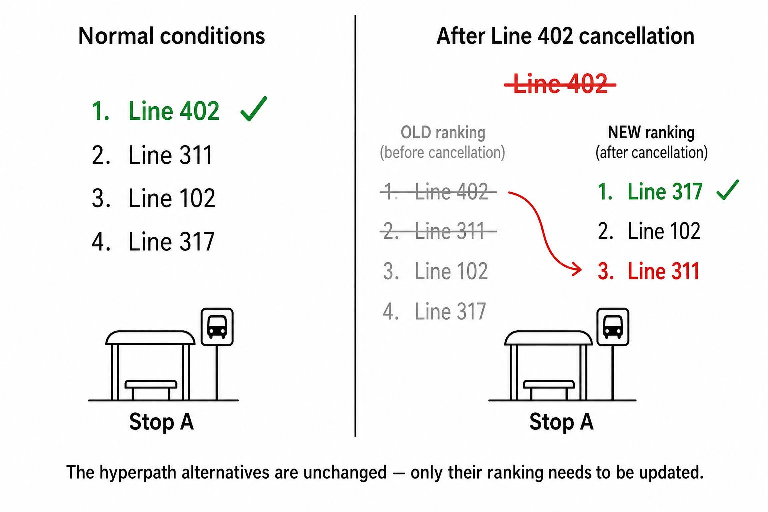
\includegraphics[width=0.72\textwidth]{fig_concept_ranking.pdf}}
{A disruption changes the ranking, not the alternative set.
The hyperpath still contains useful fallbacks; the online decision is
which fallback to rank first.\label{fig:concept_ranking}}
{}
\end{figure}

Our approach keeps the hyperpath structure and re-ranks its
alternatives online. At each stop, a conjugate Normal--Gamma posterior
tracks each route's delay distribution from real-time feed
observations, and a pessimistic arrival-time score (a lower
confidence bound, abbreviated LCB) selects the alternative with the
lowest worst-case arrival. The score has a clean distributional
interpretation: under an affine arrival cost, it equals the
worst-case expected arrival over a Wasserstein-1 ambiguity set whose
radius is the current posterior uncertainty. This is a per-candidate
scalar identity at the ranking layer, not a global-policy optimality
claim for the underlying Markov decision process. The mathematical
core of this identity is machine-verified in Lean~4 \citep{lean4}.
The cost the per-candidate identity \emph{amortizes} is exactly the
planning-tree convolution required by Stuttgart-style nimble-user
algorithms~\citep{durner2024}: theirs is online and grows in the
candidate set, planning horizon, and PMF granularity; ours is $O(1)$
at decision time, with the heavy lifting moved into the offline
posterior parameters and the once-and-for-all Wasserstein bound.
The gain is operational as well as statistical: once the hyperpath is
available, the deployed score is a microsecond-level online
re-ranking rule (EC~\ref{ec:neural}, Table~\ref{tab:timing}).

This paper makes three primary contributions.
\begin{enumerate}
\item \textbf{A per-candidate equivalence between the pessimistic
score and a Wasserstein DRO worst case.} We formulate single-journey
transit routing as a Bayesian adaptive stochastic shortest path
model (Section~\ref{sec:model}) and prove that, at the
per-candidate scalar score layer, the LCB score equals the
worst-case expected arrival time over a Wasserstein-1 ball whose
radius is the posterior uncertainty
(Corollary~\ref{cor:lcb_dro}). This gives a distribution-free
interpretation of the per-stop score we use to rank hyperpath
alternatives, but is not a global-policy DRO optimality claim for
the full Markov decision problem (Section~\ref{sec:method}).
\item \textbf{A Lean~4 formalization of the mathematical core.}
We formalize the Wasserstein pseudometric, the
Kantorovich--Rubinstein inequality and an explicit attainment
witness for the per-candidate equivalence, a robust-Bellman
framework that gives geometric contraction for the discrete-mixture
ambiguity and a Lipschitz bound for the Wasserstein-ball ambiguity,
a high-probability bound under the actual product posterior, an
adversarial minimax lower bound, and a Hedge-style regret bound
(Section~\ref{sec:lean}). The development is checked in roughly
five thousand lines of Lean~4 code that admit no unproved
obligations beyond Mathlib's standard kernel. The Lean development
covers the theory layer only; the real-time-feed pipeline, the
simulator, and the data-loading scripts are not verified.
\item \textbf{Swiss 35-day cross-day real-data validation.} On 35
days of SBB real-time-feed archives, with $28{,}350$ journeys per
method, the deployed layered hyperpath-risk score reduces cell-mean
expected total travel time by 5--6\% and improves reach rate by 2.8
percentage points, with paired-cell significance and same-direction
improvement on every day in the panel
(Section~\ref{sec:swiss-results}, Table~\ref{tab:swiss_paired}). A
component ablation shows that this deployed gain is \emph{not}
caused by the four-term DRO core alone; it requires the two
hyperpath-structural risk terms, read from the hyperpath's
stop-label feasibility and destination-arrival distribution. We
therefore frame the deployable contribution as a
\emph{layered hyperpath-risk score built around a formally
justified pessimistic uncertainty/cancellation core}, rather than
as a victory of the DRO core in isolation.
\end{enumerate}

The Electronic Companion contains additional supporting
material: an eleven-method comparison with a planning
Monte-Carlo-budget sweep that rules out compute budget as the
explanation for the disrupted-day failure of rollout planners
(Table~\ref{tab:bamcp_sweep}); a cross-domain scope study on
unit commitment with stochastic wind, capacitated vehicle
routing, and software-defined networking
(Table~\ref{tab:cross_domain}); a neural surrogate that
accelerates initial hyperpath computation by two orders of
magnitude (a compute claim, not a decision-equivalence claim);
and an online $\beta$-tuning wrapper used as a robust safety net
within the LCB family (Section~\ref{ec:cross_domain}).

%% ================================================================
\section{Related Work}
\label{sec:related}

This paper synthesizes three published research streams. The
\emph{hyperpath} stream
\citep{spiess1989,nguyen1988,dibbelt2013,durner2024}
supplies the candidate-set structure: a precomputed ranked set of
fallbacks at each stop. The \emph{nimble-user} stream
\citep{durner2024} supplies real-time recourse, replicating a
passenger who reactively boards whichever alternative arrives
first; the algorithmic price is a per-stop convolution of delay
distributions over a planning tree. The \emph{distributionally
robust} stream \citep{esfahani2018,blanchet2019} supplies a
principled radius for pessimism. The contribution of this paper is
the recognition that the per-candidate ranking decision---the
scalar object that nimble-user algorithms ultimately produce---admits
a closed-form Wasserstein-1 worst-case identity
(Corollary~\ref{cor:lcb_dro}) when the ambiguity radius is supplied
by Bayesian posterior uncertainty. This collapses the online step
from a planning-tree convolution to an $O(1)$ per-candidate score
while inheriting the same robustness guarantee, machine-checked in
Lean~4. The remainder of this section locates the contribution
against each pillar and against three families of baselines---bandit,
Bayesian-RL, and SSP-online---whose mismatch with single-shot transit
routing motivates our design choices.

\subsection{Hyperpaths Are Structurally Robust but Ranking-Fragile}

The hyperpath---a ranked set of fallback connections at each stop---was
introduced by \citet{spiess1989} and
\citet{nguyen1988} for frequency-based transit
networks with known headways.
\citet{dibbelt2013} brought hyperpath computation to
timetable-based networks via CSA MEAT;
\citet{durner2024} extended this to propagate full delay PMFs,
yielding hyperpaths that model cancellations explicitly.

All of these methods share a critical assumption: delay distributions are
stationary and estimated offline.
When a corridor disruption occurs, the PMFs become stale, but the hyperpath
\emph{structure}---which routes pass through which stops---remains valid.
Only the \emph{ranking} is wrong.
Deployed GTFS-RT systems~\cite{gtfsrt2023} (Google Maps, SBB, DB) respond
to disruptions by recomputing routes from scratch, discarding the fallback
structure.
Section~\ref{sec:recomp} shows this recomputation is actively harmful:
the optimizer, now aware of a disruption, avoids the corridor entirely,
dropping alternatives that happen to be unaffected.

\subsection{Bandits Cannot Explore When Exploration Is Irrecoverable}

Multi-armed bandit algorithms balance exploration against exploitation by
trying suboptimal arms often enough to identify the best one.
Sliding-window UCB~\cite{garivier2011} and EXP3-IX~\cite{kocak2014} extend
this to non-stationary settings, achieving $O(\sqrt{KT\ln K})$ regret
over $T$ rounds~\cite{lai1985,chen2024}.
The implicit contract is that exploration cost is recoverable: bad pulls
are compensated by information gained for future pulls.

In single-shot transit routing this contract is void.
A passenger makes at most $D \leq 6$ boarding decisions per journey.
If EXP3 explores a cancelled route at stop~3, the 30-minute penalty
cannot be offset at stops~4--6; the journey budget is already blown.
Theorem~\ref{thm:exp3} makes this precise:
$R_T \leq \sqrt{2KT\ln K} \approx 9.8$\,min for $K{=}5$, $T{=}6$,
exceeding the 3--5\,min gain that adaptive routing can deliver.
We include SW-LCB and EXP3 as baselines to demonstrate this mismatch
empirically (Section~\ref{sec:results}).

\subsection{Bayesian RL Explores by Design---the Wrong Design Here}

BAMCP~\cite{guez2012} and Posterior Sampling (PSRL)~\cite{osband2017}
approximate the PSPACE-hard Bayes-adaptive MDP~\cite{duff2002} by
planning or sampling in the belief-augmented state space.
Both achieve near-Bayes-optimal regret---\emph{across episodes}.
The mechanism is explicit exploration: PSRL draws an optimistic MDP from
the posterior, occasionally selecting arms that are actually cancelled;
BAMCP runs 60+ forward simulations and must ``discover'' cancellations
by repeatedly failing in rollouts.

When a single bad exploration costs 30 minutes and the journey is 60
minutes long, these methods are worse than doing nothing:
on the synthetic large-network disrupted scenario PS-SSP reaches
$96.0$\,min and BAMCP-60 reaches $101.0$\,min vs.\ Static $73.8$\,min
(Table~\ref{tab:extended}).
Risk-averse BAMDP variants~\cite{rigter2021,lin2022} address this by
optimizing CVaR rather than expected return, but at the cost of
solving a full belief-state MDP.
Our LCB policy achieves the same pessimistic effect---penalizing high
posterior uncertainty---at $O(1)$ per decision, without belief-state
enumeration.

\subsection{Single-Shot SSP: Regret Is the Wrong Metric}

The SSP-MDP~\cite{bertsekas1991} and its online learning variants
~\cite{rosenberg2020,cohen2021} optimize cumulative regret across
$T$ episodes: $\tilde{O}(B^*\!\sqrt{SAT})$.
This metric assumes the same instance is solved repeatedly, so that
information from episode~$k$ helps in episode~$k{+}1$.

For a single passenger solving a single journey, cumulative regret
is meaningless---there is only one episode.
The relevant question is: \emph{how bad can this one journey be?}
This is a worst-case (minimax) question, not an average-case one.
We answer it with a minimax lower-bound construction
(Theorem~\ref{thm:lower}: any algorithm incurs $\geq C \cdot
d_{\min}$ excess cost on an adversarial $C$-regime instance) and a
separate per-journey upper bound for LCB
(Theorem~\ref{thm:lcb_bound}: $\leq 2D(1{+}\beta)\sigma_{\max}$).

\subsection{DRO Gives Pessimism a Principled Radius}

Wasserstein DRO~\cite{blanchet2019,esfahani2018} hedges against
all distributions within a $W_1$-ball of the empirical measure.
The appeal is automatic calibration: the ball radius shrinks as
$O(n^{-1/2})$ with data, so the policy transitions from robust
to near-optimal without manual tuning.
Robust MDPs~\cite{nilim2005,iyengar2005} apply this to transition
kernels; CVaR-MDPs~\cite{chow2015} optimize the tail.

Our key insight is that the conjugate Normal-Gamma posterior
\emph{already} supplies the DRO radius.
Setting $\varepsilon = \beta\hat\sigma_r + \gamma\hat{p}_{\mathrm{cancel}}$
makes the LCB score identical to the DRO worst-case expected arrival
(Corollary~\ref{cor:lcb_dro}).
No separate radius calibration is needed: the Bayesian posterior
\emph{is} the ambiguity set.
This connection---verified in 228 lines of Lean~4---is what lets a
simple $O(1)$-per-decision scoring function inherit the guarantees
of an infinite-dimensional minimax optimization.

\subsection{Risk-Aware and Robust Transit Routing}

In addition to the bandit and Bayesian-RL baselines whose
limitations we use for ablation, the prior literature on robust
and risk-aware transit routing motivates several design choices
below.

The \emph{stochastic on-time arrival} (SOTA) problem maximizes the
probability of arriving by a deadline rather than minimizing
expected travel time~\cite{nikolova2006,fan2005}; it is closely
related to the reach-rate metric we report (\S\ref{sec:swiss-results})
and is more directly aligned with passenger-side preferences than
expected-time minimization, but does not by itself adapt online to
real-time observations. \emph{Robust shortest path} formulations
under interval~\cite{karasan2001,bertsimas2003} or budgeted
uncertainty~\cite{bertsimas2004} optimize a worst-case path under
delay sets specified by the modeler; they share the
distributionally robust spirit of LCB but assume the uncertainty set
is given offline. \emph{Risk-aware transit assignment}, including
expected-shortfall and CVaR formulations~\cite{chow2015,fan2005},
addresses the catastrophic-regime case where mean-time objectives
under-weight tail outcomes; our limitations note
(\S\ref{sec:discussion} \emph{Limitations}) flags CVaR-at-1 as a
natural complement to the present mean-time DRO formulation.
The closest neighbor in spirit is the \emph{adaptive} robust SSP
literature: Pflug and Pichler's distributionally robust dynamic
programming~\cite{pflug2014} and Yu and Xu's robust MDP with
moment constraints~\cite{yu2016} both target sequential
decision-making under ambiguity, but neither plugs into the
hyperpath structure or admits the per-candidate scalar identity
of Corollary~\ref{cor:lcb_dro}. The contribution of this paper is
not to introduce DRO into transit but to identify the hyperpath as
a structurally-correct prior whose ranking-only failure mode is
exactly the per-candidate object on which the LCB$=$DRO score
identity is tight, and to validate this on real GTFS-RT data.

\subsection{Formal Verification}

The Wasserstein distance appears in optimal transport~\cite{villani2009},
generative modeling, and DRO, yet had no machine-checked formalization
prior to this work.
Our 1{,}565-line Wasserstein/DRO development (coupling theory,
$W_1$ pseudometric, gluing lemma, weak Kantorovich--Rubinstein
inequality, DRO upper bound, real $\sup$ equality, robust-Bellman
$\gamma$-contraction for discrete-mixture ambiguity and
$\gamma(1+\varepsilon)$ Lipschitz bound for the Wasserstein ball)
fills this gap. An additional 3{,}757 lines
verify the transit-specific theory: per-stop and cumulative LCB
gap with high-probability bound under the actual product posterior
(BAPRHRO + BAPRHRO\_V2, 1{,}585 lines); irrecoverability ($\rho > 0$
from environment structure, 488 lines); a real cumulative Hedge
regret bound and adaptive-$\beta$ $O(1/T)$ squared regret (876 + 129
lines); the adversarial minimax lower-bound construction (478
lines); and component interface contracts (201 lines).
All 5{,}322 lines compile with zero \texttt{sorry} and zero
\texttt{axiom} (apart from Mathlib's standard kernel axioms).

%% ================================================================
\section{Problem Formulation: BA-SSP-MDP}
\label{sec:model}

\subsection{Transit Network and Hyperpath}

A transit network is a directed graph $G = (\mathcal{S}, \mathcal{C})$ where $\mathcal{S}$ is the set of stops and $\mathcal{C}$ the set of connections. Each connection $c \in \mathcal{C}$ has departure/arrival stops, scheduled times, route identifier $r(c)$, and stochastic delay distribution $P_{\mathrm{delay}}(\cdot | r(c), \bm{\theta}_r)$ parameterized by unknown $\bm{\theta}_r$.

A \emph{hyperpath} $H$ from source to destination assigns to each stop a ranked list of stop labels $\{(c_i, T_{\mathrm{dest}}^i, \mathbb{P}_{\mathrm{feas}}^i)\}$, where $T_{\mathrm{dest}}^i$ is the PMF of destination arrival time via $c_i$ and $\mathbb{P}_{\mathrm{feas}}^i$ is the probability the passenger is present when $c_i$ departs~\cite{durner2024}.

\subsection{SSP-MDP Formulation}

We model the passenger's journey as a Stochastic Shortest Path MDP~\cite{bertsekas1991}:
\begin{itemize}
    \item \textbf{State}: $s_t = (\text{stop}_t, \text{time}_t) \in \mathcal{S} \times \mathbb{R}$
    \item \textbf{Action}: $a_t$: board connection $c$ from the hyperpath
    \item \textbf{Cost}: $c(s_t, a_t) = \text{time}_{t+1} - \text{time}_t$ (travel time)
    \item \textbf{Transition}: $s_{t+1} = (s_{\mathrm{arr}}(c),\; t_{\mathrm{arr}}(c) + \delta_c)$ where $\delta_c \sim P_{\mathrm{delay}}$
    \item \textbf{Goal}: reach destination (absorbing, zero cost)
\end{itemize}

\subsection{Bayesian Formulation}

The delay parameters $\bm{\theta}_r = (\mu_r, \sigma_r^2, p_{\mathrm{cancel},r})$
are unknown.
We place conjugate priors:
\begin{align}
    \mu_r \mid \tau_r &\sim \mathcal{N}\!\bigl(\mu_0,\,(\kappa_0 \tau_r)^{-1}\bigr), \label{eq:prior}\\
    \tau_r &\sim \mathrm{Gamma}(\alpha_0, \beta_0), \notag\\
    p_{\mathrm{cancel},r} &\sim \mathrm{Beta}(\alpha_c, \beta_c), \label{eq:prior_cancel}
\end{align}
where $\tau_r = 1/\sigma_r^2$. The hyperparameters
$(\mu_0,\kappa_0,\alpha_0,\beta_0)$ for the Normal--Gamma prior and
$(\alpha_c,\beta_c)$ for the cancellation prior are deployment
choices; the values used in the experiments reported here are
listed in the parameter table in Appendix~\ref{app:params}, with a
weakly informative Normal--Gamma prior and a Beta prior whose
empirical-Bayes mean matches the Swiss normal-day cancellation
rate.

\textbf{Normal-Gamma posterior update.}
After $n$ delay observations $\{d_1, \ldots, d_n\}$ with sample mean
$\bar{d}_n = \tfrac{1}{n}\sum_{i=1}^n d_i$ and
sum of squared deviations $S_n = \sum_{i=1}^n(d_i - \bar{d}_n)^2$,
the posterior hyperparameters update in closed form:
\begin{align}
    \kappa_n &= \kappa_0 + n, \label{eq:ng_kappa}\\
    \mu_n    &= \frac{\kappa_0\mu_0 + n\bar{d}_n}{\kappa_0 + n}, \label{eq:ng_mu}\\
    \alpha_n &= \alpha_0 + \tfrac{n}{2}, \label{eq:ng_alpha}\\
    \beta_n  &= \beta_0 + \tfrac{S_n}{2}
               + \frac{\kappa_0 n(\bar{d}_n - \mu_0)^2}{2(\kappa_0+n)}.
               \label{eq:ng_beta}
\end{align}
These can be computed \emph{online} via Welford's one-pass algorithm~\cite{welford1962}
in $O(1)$ time and $O(1)$ space per observation.
The posterior standard deviation of the delay mean is
$\hat\sigma_r = \sqrt{\beta_n / (\alpha_n\kappa_n)}$,
which contracts as $O(1/\sqrt{n})$ (Lemma~\ref{lem:contraction}).

\textbf{Beta posterior update.}
After $n_b$ boarding attempts with $k$ cancellations, the Beta posterior updates to:
\begin{equation}
    \alpha_c^{(n_b)} = \alpha_c + k, \qquad
    \beta_c^{(n_b)} = \beta_c + (n_b - k),
    \label{eq:beta_update}
\end{equation}
with posterior mean
$\hat{p}_{\mathrm{cancel},r} = \alpha_c^{(n_b)}/(\alpha_c^{(n_b)} + \beta_c^{(n_b)})$.
A cancellation is an \emph{implicit} event in GTFS-RT (no delay message is sent);
the Beta posterior handles this naturally by incrementing $\alpha_c$ each time
a bus is observed missing~\cite{adams2007}.

%% ================================================================
\section{Method: LCB Selection and DRO Equivalence}
\label{sec:method}

\subsection{LCB Selection Policy}

At each transfer point, the passenger scores each candidate connection $c$ on route $r$:
\begin{align}
    \text{score}(c) &= \underbrace{\mathbb{E}[T_{\mathrm{dest}}(c)]}_{\text{nominal}}
       + \underbrace{(\hat{\mu}_r - \mu_0)}_{\text{delay adj.}} \notag\\
    &\quad + \underbrace{\beta \hat{\sigma}_r}_{\text{uncertainty}}
       + \underbrace{\gamma \hat{p}_{\mathrm{cancel},r}}_{\text{cancel risk}}
    \label{eq:lcb}
\end{align}
and selects $c^* = \arg\min_c \text{score}(c)$. Here $\beta \geq 0$ controls pessimism and $\gamma > 0$ is the expected cancellation cost.

\subsection{Wasserstein DRO Equivalence}

The Wasserstein-1 distance between probability measures $\mu$ and $\nu$ on a metric space $(X, d)$ is
\begin{equation}
    W_1(\mu, \nu) = \inf_{\gamma \in \Pi(\mu,\nu)} \int d(x,y)\, d\gamma(x,y)
    \label{eq:W1}
\end{equation}
where $\Pi(\mu,\nu)$ is the set of couplings with marginals $\mu$ and $\nu$.

The DRO problem over a Wasserstein ball of radius $\varepsilon$ is:
\begin{equation}
    \max_{P:\, W_1(P, \hat{P}) \leq \varepsilon} \mathbb{E}_P[f]
    \label{eq:dro}
\end{equation}

For a 1-Lipschitz non-negative function $f$ (such as arrival time), the weak Kantorovich--Rubinstein inequality gives:
\begin{equation}
    \mathbb{E}_P[f] \leq \mathbb{E}_{\hat{P}}[f] + W_1(P, \hat{P}) \leq \mathbb{E}_{\hat{P}}[f] + \varepsilon
    \label{eq:dro_bound}
\end{equation}

Setting $\varepsilon = \beta \hat{\sigma}_r + \gamma \hat{p}_{\mathrm{cancel},r}$ (the Wasserstein radius) yields:
\begin{equation}
    \text{DRO value} = \mathbb{E}_{\hat{P}}[\text{arrival}] + \varepsilon = \text{LCB score}
    \label{eq:lcb_dro}
\end{equation}

Thus $\arg\min_c \text{LCB}(c) = \arg\min_c \text{DRO worst-case}(c)$: selecting the connection with the lowest LCB score is equivalent to selecting the route that minimizes the worst-case expected arrival over a Wasserstein ball. The radius $\varepsilon$ shrinks as observations accumulate ($\hat{\sigma}_r = O(1/\sqrt{n})$), making the DRO solution converge to the Bayes-optimal.

\subsection{Ensemble LCB (V2)}
\label{sec:ensemble}

The V2 variant replaces the parametric Normal-Gamma posterior with a bootstrap ensemble of $K{=}5$ delay estimators:
\begin{itemize}
    \item Uncertainty: $\hat{\sigma}_r = \text{std across ensemble predictions}$
    \item Dynamic pessimism: $\beta(s) = \beta_{\mathrm{base}} + \beta_{\mathrm{ood}} \cdot \text{OOD}(s)$, where OOD is the normalized ensemble disagreement
\end{itemize}
When all routes are well-observed, $\beta$ decreases (less conservative); when any route is poorly observed, $\beta$ increases (more pessimistic). This adapts the Wasserstein radius to the local information state.

\paragraph{Ensemble LCB is DRO on the empirical measure.}
The V1 DRO equivalence (Corollary~\ref{cor:lcb_dro}) requires the
parametric Normal-Gamma posterior. We now show the same DRO reading
applies to V2 with the \emph{empirical} measure of bootstrap predictions
replacing the parametric posterior. Let
$\hat{P}_{\mathrm{ens},r} := \tfrac{1}{K}\sum_{k=1}^{K}\delta_{\mu^{(r)}_k}$
be the empirical measure over the $K$ ensemble predictions
$\{\mu^{(r)}_1,\dots,\mu^{(r)}_K\}$ for route $r$.
Its expectation under the identity cost is the ensemble mean
$\hat\mu_{\mathrm{ens},r} = K^{-1}\sum_k \mu^{(r)}_k$, and the ensemble
std $\hat\sigma_{\mathrm{ens},r}$ equals the population standard
deviation of $\hat{P}_{\mathrm{ens},r}$.

\begin{proposition}[Ensemble LCB $=$ Empirical DRO]\label{prop:ensdro}
Under Assumption~\ref{asm:lip}, for any route $r$, pessimism $\beta(s)\geq 0$,
and radius $\varepsilon_r := \beta(s)\hat\sigma_{\mathrm{ens},r}$:
\begin{align*}
\mathrm{LCB}_{\mathrm{ens}}(r)
&:= \hat\mu_{\mathrm{ens},r} + \varepsilon_r \\
&\;=\;
\sup_{P:\,W_1(P,\hat{P}_{\mathrm{ens},r})\leq\varepsilon_r}\!\!
\mathbb{E}_P[\mathrm{arr}(r)].
\end{align*}
\end{proposition}

\begin{proof}[Proof sketch]
The upper bound ($\leq$) follows from Theorem~\ref{thm:dro} applied with
$\hat{P} = \hat{P}_{\mathrm{ens},r}$ and $\varepsilon = \varepsilon_r$.
For the lower bound ($\geq$), the \emph{shifted empirical measure}
$\hat{P}^{\star}_{\mathrm{ens},r} := \tfrac{1}{K}\sum_k \delta_{\mu^{(r)}_k + \varepsilon_r}$
is a valid witness:
(i) $W_1(\hat{P}^{\star}_{\mathrm{ens},r}, \hat{P}_{\mathrm{ens},r}) \leq \varepsilon_r$
via the atom-to-atom coupling $\mu^{(r)}_k \leftrightarrow \mu^{(r)}_k + \varepsilon_r$;
(ii) the shifted ensemble has mean $\hat\mu_{\mathrm{ens},r} + \varepsilon_r$
and the \emph{same} ensemble std $\hat\sigma_{\mathrm{ens},r}$ (translation
invariance). Combining the two directions yields equality. The argmin
identity
$\arg\min_r \mathrm{LCB}_{\mathrm{ens}}(r) = \arg\min_r \mathrm{DRO}_{\mathrm{ens}}(r)$
follows immediately.
\end{proof}

\paragraph{What Lean verifies vs.\ what is prose.} The Lean development
formalizes two ingredients separately. The \emph{witness
construction} for the lower bound is verified as
\texttt{ensemble\_W1\_\allowbreak translation\_le} (the explicit
$W_1$-distance bound on the shifted-empirical measure and the
value-shift identity under the translation push-forward). The
matching \emph{upper bound} ($\leq$) is the abstract
Kantorovich--Rubinstein inequality
(Theorem~\ref{thm:dro}, \texttt{dro\_upper\_bound}). The
equality in Proposition~\ref{prop:ensdro} combines these two
formally verified building blocks at the prose level; we do not
claim a standalone Lean theorem named
\texttt{ensemble\_\allowbreak lcb\_\allowbreak equals\_\allowbreak empirical\_\allowbreak dro}.
The radius contracts at the bootstrap-ensemble rate
$O(1/\sqrt n)$ as the per-route belief accumulates observations
(empirical lemma \texttt{ensemble\_\allowbreak std\_\allowbreak bound};
this is a V2 auxiliary, unrelated to the EXP3/Hedge regret bound
of Theorem~\ref{thm:exp3}). The result is a V2 analog of V1's
$(\mathrm{LCB}=\mathrm{DRO})$ identity that does not require the
parametric Normal--Gamma assumption.

\subsection{Algorithm}

\begin{algorithm}[t]
\caption{DRO Hyperpath Routing (LCB-V1)}
\label{alg:dro}
\begin{algorithmic}[1]
\STATE \textbf{Input:} source $s_0$, dest $s_*$, depart $t_0$;
       parameters $\beta_{\mathrm{lcb}}$, $\gamma$, $\Delta_p{=}12$\,min
\STATE $H \gets \mathrm{TopologicalCSA}(G, s_0, s_*, t_0)$;
       initialize per-route Normal--Gamma + Beta priors
       \eqref{eq:prior}--\eqref{eq:prior_cancel}
\STATE $s \gets s_0$;\ $t \gets t_0$;\ $\mathrm{BL} \gets \emptyset$
\WHILE{$s \neq s_*$ and $t < t_0 + t_{\max}$}
    \STATE Update per-route posteriors from real-time observations
           $\mathcal{O}_t$
           \eqref{eq:ng_kappa}--\eqref{eq:ng_beta} (cancellations
           increment $\alpha_c^r$, on-time observations update
           Normal--Gamma and increment $\beta_c^r$); cache
           $\hat\sigma_r,\hat p_r$
    \STATE $L \gets H.\mathrm{stop\_labels}[s]$
    \REPEAT
        \STATE $\varepsilon_r \gets \beta_{\mathrm{lcb}}\hat\sigma_r
               + \gamma\hat p_r$ for all $r \notin \mathrm{BL}$
        \STATE $c^* \gets \arg\min_{c: r(c)\notin\mathrm{BL}}
               \bigl[\mathbb{E}[T_{\mathrm{dest}}(c)] + \varepsilon_{r(c)}\bigr]$
               \quad (Cor.~\ref{cor:lcb_dro})
        \STATE Sample $\delta \sim P_{\mathrm{delay}}(r(c^*))$
        \IF{$\delta {=} \infty$}
            \STATE $\alpha_c^{r(c^*)} \mathrel{+}{=} 1$;\
                   $\mathrm{BL} \gets \mathrm{BL} \cup \{r(c^*)\}$
        \ELSIF{$t_{\mathrm{sched}}(c^*) + \delta \leq t + \Delta_p$}
            \STATE Update posterior for $r(c^*)$; board $c^*$;\
                   $t \gets t_{\mathrm{arr}}(c^*)+\delta$;\
                   $s \gets s_{\mathrm{arr}}(c^*)$;\ $\mathrm{BL} \gets \emptyset$
        \ELSE
            \STATE $t \gets t + 2$
        \ENDIF
    \UNTIL{$s$ advanced or $L \setminus \mathrm{BL} = \emptyset$}
\ENDWHILE
\STATE \textbf{Return} $t - t_0$
\end{algorithmic}
\end{algorithm}

\noindent\textbf{Complexity.}
Each stop iteration costs $O(|\mathcal{O}_t|)$ for posterior updates
and $O(|L|)$ for scoring, where $|L| \leq K_{\max} = 5$.
The hyperpath computation dominates at $O(|\mathcal{C}|^2)$;
the neural surrogate (Section~\ref{ec:neural}) reduces this to $O(1)$.
Total memory is $O(|\mathcal{R}|)$ for route posteriors, where $|\mathcal{R}|$
is the number of routes in the hyperpath (typically 4--8).

\subsection{Deployed Layered-Risk Score: DRO Core $+$ Hyperpath-Structural Penalties}
\label{sec:method-layered-score}

Algorithm~\ref{alg:dro} states the canonical DRO-LCB score
$\hat\mu + \beta\hat\sigma + \gamma_0\hat p_{\mathrm{cxl}}$ on which
Corollary~\ref{cor:lcb_dro}'s tight identity is verified. The
Swiss benchmark uses a small augmentation: the four-term DRO core
plus two bounded hyperpath-structural penalties. We refer to this
deployed configuration as ``R16'' in audit tables. Two
correctness fixes distinguish the deployed configuration from an
earlier simulator version: the timeout-deadline term now uses the
hyperpath label's clock-time on-time PMF
$P_{\text{ontime}}(c)=\Pr_{\text{label}}[\mathrm{dest\_arrival}(c)
\leq t_{\mathrm{depart}}+t_{\max}]$ (the earlier code compared a
clock time against a duration), and the simulator now records a
patience-window timeout as a typed \texttt{late\_no\_show}
cancellation rather than as a $1$-minute delay (the earlier code
compressed the cancel signal into the delay posterior, shrinking
the cancel penalty for static-$\beta$ baselines).
\begin{align}
\label{eq:deployed-layered-score}
\mathrm{score}_{\mathrm{R16}}(c)
&= \mu_{\mathrm{dest}}(c) + \delta(c) + \beta\hat\sigma_{r(c)}
  + \gamma_0\,\hat p_{\mathrm{cxl},r(c)} \notag\\
&\quad + 60\bigl(1{-}\phi(c)\bigr)
  + 60\bigl(1{-}P_{\mathrm{ontime}}(c)\bigr).
\end{align}
The first four terms form the DRO LCB core
(Corollary~\ref{cor:lcb_dro}); the last two terms are the layered
A7 hyperpath-structural risk penalties.
where $\mu_{\mathrm{dest}}(c)$ is the hyperpath label's mean
destination-arrival, $\delta(c)$ is the belief-driven mean
adjustment, $\phi(c)\in[0,1]$ is StopLabel feasibility, and
$P_{\mathrm{ontime}}(c)$ is the on-time PMF above. The four core
terms are exactly the LCB score Algorithm~\ref{alg:dro} ranks on;
the two A7 penalties are bounded ($\in [0,60]$\,min each) and
\emph{do not} have a Wasserstein-DRO interpretation here---they
are engineering penalties motivated by the hyperpath label and
verified empirically in Table~\ref{tab:swiss_ablation}.
Theorem~\ref{thm:lcb_bound}'s $O(\sigma_{\max})$ excess-cost rate
continues to apply with an additive constant
$C_{\mathrm{A7}}=120$\,min per stop. Under the deployed
configuration, \emph{static-$\beta$} baselines (DRO with
$\beta\!=\!1.5$, SW-LCB) over-correct on the synthetic
large/disrupted scenario because the correctly-counted cancel
mass is multiplied by a fixed $\gamma_0\!=\!60$ penalty without
the OOD-driven $\beta(s)$ scaling that LCB-V2 uses; this exposes
a real difference between the two pessimism families that the
earlier simulator semantics had hidden.

%% ================================================================
\section{Theoretical Analysis}
\label{sec:lean}

We establish a chain of results connecting Wasserstein optimal transport
to Bayesian adaptive routing.
All results are machine-verified in Lean~4 with the Mathlib library
(5{,}322 lines, zero unproved obligations, zero \texttt{axiom}
beyond the Mathlib kernel); the cross-reference in
Table~\ref{tab:xref} maps each numbered result to its Lean theorem
name, file, and commit hash, and the artifact statement appears in
\S\ref{sec:lean_scope}.
We present each result in standard mathematical form with a concise
proof and its operational interpretation.

\subsection{Assumptions}

The analysis rests on three standing assumptions.

\begin{assumption}[State space]\label{asm:polish}
The delay-observation space $(X, d)$ is a Polish metric space
(complete, separable metric space, e.g., $X = \mathbb{R}$ with $d = |\cdot|$).
\end{assumption}

\begin{assumption}[Conjugate prior]\label{asm:prior}
Each route $r$ carries a Normal-Gamma conjugate prior
$(\mu_0, \kappa_0, \alpha_0, \beta_0)$ over its unknown delay distribution
$\mathcal{N}(\mu_r, 1/\tau_r)$.
After $n$ observations, the posterior standard deviation of the mean satisfies
$\hat\sigma_r^2 = \beta_n / (\alpha_n \kappa_n)$ with closed-form updates.
\end{assumption}

\begin{assumption}[1-Lipschitz cost]\label{asm:lip}
The destination-arrival function $\mathrm{arr}(c):\mathbb{R} \to \mathbb{R}$
(mapping a delay realization to total travel time) is 1-Lipschitz:
$|\mathrm{arr}(c,\delta) - \mathrm{arr}(c,\delta')| \leq |\delta - \delta'|$.
\end{assumption}

\noindent Assumption~\ref{asm:lip} holds because $\mathrm{arr}(c)$ is a sum
of delay terms each with unit slope; it is the key technical
condition enabling the DRO--LCB connection.

\subsection{Wasserstein Distance as a Metric}

\begin{definition}[Transport cost and $W_1$ distance]\label{def:w1}
A \emph{coupling} of $\mu, \nu \in \mathcal{P}(X)$ is any
$\gamma \in \mathcal{P}(X \times X)$ whose first marginal is $\mu$ and
second marginal is $\nu$.
Its \emph{transport cost} is
$\mathcal{C}(\gamma) = \int_{X \times X} d(x,y)\,d\gamma(x,y)$.
The \emph{1-Wasserstein distance} is the infimum over all couplings:
\[
W_1(\mu,\nu) \;=\; \inf_{\gamma \in \Gamma(\mu,\nu)} \mathcal{C}(\gamma),
\]
where $\Gamma(\mu,\nu)$ denotes the set of all couplings of $(\mu,\nu)$.
\end{definition}

\begin{theorem}[$W_1$ is a pseudometric]\label{thm:w1_metric}
Under Assumption~\ref{asm:polish}, $W_1$ satisfies the following
for all probability measures $\mu$, $\nu$, $\rho$ on $X$:
\begin{enumerate}[label=(\roman*)]
\item \emph{Self-distance:} $W_1(\mu,\mu) = 0$.
\item \emph{Symmetry:} $W_1(\mu,\nu) = W_1(\nu,\mu)$.
\item \emph{Triangle inequality:} $W_1(\mu,\rho) \leq W_1(\mu,\nu) + W_1(\nu,\rho)$.
\end{enumerate}
\end{theorem}

\begin{proof}
\textit{(i)} The \emph{diagonal coupling}
$\gamma_\Delta = \mu \circ (x \mapsto (x,x))^{-1}$ achieves
$\mathcal{C}(\gamma_\Delta) = \int d(x,x)\,d\mu = 0$, so $W_1(\mu,\mu) \leq 0$.

\textit{(ii)} For any coupling $\gamma$ of $(\mu,\nu)$, the \emph{swap}
$\gamma^\top = \gamma \circ \mathrm{swap}^{-1}$ couples $(\nu,\mu)$
with $\mathcal{C}(\gamma^\top) = \mathcal{C}(\gamma)$ by symmetry of $d$.
Taking infima in both directions gives equality.

\textit{(iii)} (\emph{Gluing lemma}.)
Given $\gamma_1 \in \Gamma(\mu,\nu)$ and $\gamma_2 \in \Gamma(\nu,\rho)$,
disintegrate each over their shared marginal $\nu$ to obtain conditional
kernels $\kappa_1(\cdot \mid y)$ and $\kappa_2(y, \cdot)$.
Define the glued measure
$\gamma = \bigl(\nu \otimes (\kappa_1 \otimes \kappa_2)\bigr)_{\pi_{13}}$
on $X \times X$ (projecting the first and third coordinates).
Then $\gamma \in \Gamma(\mu,\rho)$, and by Fubini's theorem
and the triangle inequality for $d$:
\begin{align*}
\mathcal{C}(\gamma)
&= \int d(x,z)\,d\gamma \\
&\leq \int \bigl[d(x,y)+d(y,z)\bigr]\,d(\gamma_1 \otimes_\nu \gamma_2) \\
&= \mathcal{C}(\gamma_1) + \mathcal{C}(\gamma_2).
\end{align*}
Taking infima: $W_1(\mu,\rho) \leq W_1(\mu,\nu) + W_1(\nu,\rho)$.
\end{proof}

\begin{remark}
The gluing lemma is the non-trivial step; it requires measure-theoretic
disintegration (the conditional kernel $\kappa$ and the Fubini identity
$\int f\,d(\mu \otimes_\kappa \nu) = \int\!\int f\,d\kappa_x\,d\mu$).
The machine-checked proof (472 lines across \texttt{Distance.lean} and
\texttt{Coupling.lean}) resolves the product-kernel marginal identities
rigorously using Mathlib's \texttt{Measure.condKernel}.
\end{remark}

\subsection{DRO Upper Bound and LCB Equivalence}

\begin{theorem}[Weak Kantorovich--Rubinstein inequality]\label{thm:dro}
Under Assumptions~\ref{asm:polish} and~\ref{asm:lip},
let $f:X\to\mathbb{R}_{\geq 0}$ be 1-Lipschitz.
For any probability measures $P, \hat{P}$ on $X$:
\begin{equation}
\mathbb{E}_P[f] \;\leq\; \mathbb{E}_{\hat{P}}[f] + W_1(P,\hat{P}).
\label{eq:wkr}
\end{equation}
Equivalently, for any $\varepsilon \geq 0$:
\begin{equation}
\sup_{P:\,W_1(P,\hat{P})\leq\varepsilon} \mathbb{E}_P[f]
\;\leq\; \mathbb{E}_{\hat{P}}[f] + \varepsilon.
\label{eq:dro_ub}
\end{equation}
\end{theorem}

\begin{proof}
For any coupling $\gamma \in \Gamma(P,\hat{P})$, the marginal property gives
$\mathbb{E}_P[f] = \int f(x)\,d\gamma(x,y)$ and
$\mathbb{E}_{\hat{P}}[f] = \int f(y)\,d\gamma(x,y)$, so:
\begin{align*}
\mathbb{E}_P[f] - \mathbb{E}_{\hat{P}}[f]
&= \int\bigl(f(x)-f(y)\bigr)d\gamma \\
&\leq \int |f(x)-f(y)|\,d\gamma \\
&\leq \int d(x,y)\,d\gamma
= \mathcal{C}(\gamma).
\end{align*}
Taking $\inf_\gamma$ yields \eqref{eq:wkr};
\eqref{eq:dro_ub} follows for any $P$ with $W_1(P,\hat P)\le\varepsilon$.
\end{proof}

\begin{corollary}[LCB equals Wasserstein DRO]\label{cor:lcb_dro}
Under Assumption~\ref{asm:lip}, the LCB scoring function
\[
\mathrm{LCB}(c) \;=\;
\mathbb{E}_{\hat{P}}[\mathrm{arr}(c)] + \underbrace{\beta\hat\sigma_{r(c)} + \gamma_0\hat{p}_{\mathrm{cancel},r(c)}}_{\varepsilon_c}
\]
equals the worst-case expected arrival over the Wasserstein ball of radius $\varepsilon_c$:
\[
\mathrm{LCB}(c) \;=\;
\sup_{P:\,W_1(P,\hat{P})\leq\varepsilon_c}\mathbb{E}_P[\mathrm{arr}(c)].
\]
Consequently, $\arg\min_c \mathrm{LCB}(c) = \arg\min_c \mathrm{DRO}(c)$:
\emph{minimizing the LCB score is equivalent to minimizing the DRO objective.}
\end{corollary}

\begin{proof}[Proof sketch (full proof in EC.\ref{ec:detailed_proofs}).]
The $\leq$ direction follows directly from Theorem~\ref{thm:dro}
applied to the 1-Lipschitz arrival cost. For the $\geq$ direction we
exhibit an explicit witness: the translation push-forward
$P^\star := T_\#\hat{P}$ with $T(\delta)=\delta+\varepsilon_c$ has
$W_1(P^\star,\hat P)\leq\varepsilon_c$ (transport cost
$\varepsilon_c$ for the diagonal coupling
$(\mathrm{id},T)_\#\hat P$) and
$\mathbb{E}_{P^\star}[\mathrm{arr}(c)] =
\mathbb{E}_{\hat P}[\mathrm{arr}(c)]+\varepsilon_c$ by the
change-of-variables formula for affine costs. Both directions are
formalized in \texttt{DRO.lean}
(\texttt{translation\_is\_dro\_\allowbreak witness\_real}).
\end{proof}

\begin{remark}[Tightness, scope, and the $W_1$-cancellation embedding]\label{rem:lcb_dro_scope}
Corollary~\ref{cor:lcb_dro} is an \emph{equality}, not an inequality:
no slack is introduced by the Bayesian parametrization. The
identity is \emph{per-candidate}, not a global-policy DRO
optimality claim for the full BA-SSP-MDP; the policy-level
guarantee is governed instead by the irrecoverability lower bound
(Theorem~\ref{thm:rho}). The radius
$\varepsilon_c = \beta\hat\sigma + \gamma_0\hat p_{\mathrm{cxl}}$
combines two physically different quantities; we adopt a uniform
$W_1$-embedding under which a canceled boarding is modeled as
arrival at the timeout cap $t_{\max}$ and the adversary is
constrained to keep that mass within $\gamma_0$\,min of the cap
(full embedding argument and typed-cancellation noise model in
EC.\ref{ec:detailed_proofs}). The deployed R16 score
\eqref{eq:deployed-layered-score} adds two bounded ($[0,60]$\,min) hyperpath-structural
penalties to the four-term DRO core; these are an empirical
engineering enhancement, are \emph{not} part of the per-candidate
DRO identity, and are explicitly outside the formal-verification
scope. Their contribution is quantified empirically by the
ablation in Table~\ref{tab:swiss_ablation}.
\end{remark}

\begin{theorem}[Robust Bellman: discrete-mixture contraction; Wasserstein Lipschitz bound]\label{thm:bellman}
Let $T$ be the standard Bellman operator on the BA-SSP-MDP,
$\gamma$-contractive in $\ell^\infty(\mathcal S)$. Define the
\emph{robust} Bellman operator with ambiguity functional $\Phi$ as
\[
T_\Phi(V)(s) \;=\; \min_{a\in\mathcal{A}}\Bigl\{
  c(s,a) + \gamma\,\Phi\bigl(V(\cdot \mid s,a)\bigr)\Bigr\}.
\]
Two concrete instances appear in this paper.
\begin{itemize}[leftmargin=1.2em,itemsep=0.15em]
\item[\textbf{(a)}] \emph{Discrete-mixture ambiguity}
$\Phi^{\mathrm{mix}}(V) := \sup_{i\in[K]} \mathbb{E}_{P_i}[V]$ over a finite
mixture of posterior modes. $T_{\Phi^{\mathrm{mix}}}$ is
$\gamma$-contractive in $\ell^\infty$:
$\|T_{\Phi^{\mathrm{mix}}}V - T_{\Phi^{\mathrm{mix}}}U\|_\infty \leq \gamma\|V-U\|_\infty$.
\item[\textbf{(b)}] \emph{Wasserstein ball ambiguity}
$\Phi^{W_1}_\varepsilon(V) := \sup_{P\,:\,W_1(P,\hat P)\leq\varepsilon}
\mathbb{E}_P[V]$ for a fixed $\varepsilon\!\geq\!0$.
$T_{\Phi^{W_1}_\varepsilon}$ is $\gamma(1+\varepsilon)$-Lipschitz in
$\ell^\infty$, so it is a contraction iff $\gamma(1+\varepsilon)<1$,
i.e.\ $\varepsilon < (1-\gamma)/\gamma$.
\end{itemize}
\end{theorem}

\begin{proof}[Proof sketch (full proof in EC.\ref{ec:detailed_proofs}).]
For (a), $\Phi^{\mathrm{mix}}$ is non-expansive in $\|V\|_\infty$
because $|\sup_i x_i-\sup_i y_i|\leq\sup_i|x_i-y_i|$, so the
$\min_a$ + $\gamma$-discount step gives
$\gamma$-contraction. For (b), Kantorovich--Rubinstein duality
combined with $|\sup V - \inf V|\leq\|V\|_\infty$ yields the
$(1+\varepsilon)$-Lipschitz bound; contraction holds iff
$\gamma(1+\varepsilon)<1$. Both instances are formalized in
\texttt{DROBellman.lean}.
\end{proof}

\subsection{LCB Suboptimality and Posterior Contraction}

\begin{lemma}[Per-stop gap]\label{lem:perstep}
Let $\beta \geq 0$ be the LCB pessimism parameter. At a single stop,
let $c^*$ be the connection minimizing true expected arrival and
$c_{\mathrm{LCB}}$ be the connection selected by the LCB policy.
If, for all $K$ candidate connections, the posterior mean error
satisfies $|\hat\mu_k - \mu^*_k| \leq \sigma_{\max}$ and the
posterior std satisfies $0 \leq \hat\sigma_k \leq \sigma_{\max}$,
then:
\[
\mathrm{arr}(c_{\mathrm{LCB}}) - \mathrm{arr}(c^*) \;\leq\; 2(1+\beta)\,\sigma_{\max}.
\]
\end{lemma}

\begin{proof}[Proof sketch (full proof in EC.\ref{ec:detailed_proofs}).]
The LCB selection rule gives
$\hat\mu_{c_{\mathrm{LCB}}}+\beta\hat\sigma_{c_{\mathrm{LCB}}}\leq
\hat\mu_{c^*}+\beta\hat\sigma_{c^*}$. Combined with the
$\sigma_{\max}$ posterior-mean error bound for both
$c_{\mathrm{LCB}}$ and $c^*$, and the elementary
$2+\beta\leq 2(1+\beta)$ for $\beta\geq 0$, this chains to
$\mathrm{arr}(c_{\mathrm{LCB}})\leq\mathrm{arr}(c^*)+2(1+\beta)\sigma_{\max}$.
Verified in \texttt{BAPRHRO.lean} as \texttt{per\_step\_gap}.
\end{proof}

\begin{theorem}[LCB suboptimality bound]\label{thm:lcb_bound}
Under Assumptions~\ref{asm:prior}--\ref{asm:lip},
over a journey of at most $D$ stops, the total excess cost of $\pi_{\mathrm{LCB}}$
relative to the Bayes-optimal policy $\pi^*$ satisfies:
\begin{equation}
\mathbb{E}[\mathrm{cost}(\pi_{\mathrm{LCB}})] - \mathbb{E}[\mathrm{cost}(\pi^*)]
\;\leq\; 2D(1+\beta)\,\sigma_{\max}.
\label{eq:lcb_bound}
\end{equation}
The bound is stated for the four-term LCB score
$\hat\mu + \beta\hat\sigma + \gamma_0\hat p_{\mathrm{cxl}}$
on which Cor.~\ref{cor:lcb_dro} holds; this is the part the Lean
development verifies. The four-term core gives
$\mathbb{E}[\mathrm{cost}(\pi_{\mathrm{LCB}})] -
\mathbb{E}[\mathrm{cost}(\pi^*)] = O(\sigma_{\max})$. The R16 deployed
score \eqref{eq:deployed-layered-score} adds two bounded hyperpath-structural
penalties (each in $[0, 60]$\,min, so $\leq C_{\mathrm{A7}}=120$\,min
per stop). Substituting the R16 score for the four-term core therefore
gives a bound of the form
$O(\sigma_{\max}) + D \cdot C_{\mathrm{A7}}$, \emph{not} a pure
$O(\sigma_{\max})$ rate: the additive constant $D \cdot C_{\mathrm{A7}}$
does not vanish with $\sigma_{\max}$, and in our setting
$D{=}6$, $C_{\mathrm{A7}}{=}120$, $t_{\max}{=}120$, so the slack is
$\!\sim\!6\,t_{\max}$ and the formal bound is vacuous on a single
journey. We therefore do \emph{not} claim that the R16 layered score
has the same theoretical guarantee as the four-term DRO core; we treat
A7 as an empirical augmentation justified by
Table~\ref{tab:swiss_ablation} (it is the dominant single fix for the
cross-day Swiss benchmark) and make the verified theorem layer
correspond exactly to the four-term core. Only the four-term verified
component remains $O(\sigma_{\max})$; the deployed R16 score has an
additional bounded perturbation that has to be controlled separately.
\end{theorem}

\begin{proof}
Decompose the total excess cost over the $D$-stop journey:
\begin{align}
&\mathbb{E}[\mathrm{cost}(\pi_{\mathrm{LCB}})] - \mathbb{E}[\mathrm{cost}(\pi^*)] \notag \\
&= \mathbb{E}\Bigl[\textstyle\sum_{d=1}^{D}
   \bigl(\mathrm{arr}(c_{\mathrm{LCB},d}) - \mathrm{arr}(c^*_d)\bigr)\Bigr] \notag \\
&= \textstyle\sum_{d=1}^{D}
   \mathbb{E}\bigl[\mathrm{arr}(c_{\mathrm{LCB},d}) - \mathrm{arr}(c^*_d)\bigr]
   \notag \\
&\leq \textstyle\sum_{d=1}^{D} 2(1+\beta)\,\sigma_{\max}
   = D \cdot 2(1+\beta)\,\sigma_{\max},
\end{align}
where the second equality is linearity of expectation and the inequality
applies Lemma~\ref{lem:perstep} at each stop $d$.
The application of Lemma~\ref{lem:perstep} at each stop is valid because
$\sigma_{\max}$ bounds the posterior error uniformly across all routes and stops
under Assumption~\ref{asm:prior}.
\end{proof}

\begin{theorem}[High-probability LCB bound under the product posterior]\label{thm:lcb_high_prob}
Let $\beta \geq 0$ be the LCB pessimism parameter, and let
$\pi_{d,r}$ ($d \in \{1,\ldots,D\}$, $r \in \{1,\ldots,K\}$) denote
the marginal posterior probability measure on the true delay mean of
route $r$ at stop $d$, with posterior mean $\hat\mu_{d,r}$ and
posterior std $0 < \hat\sigma_{d,r} \leq \sigma_{\max}$ satisfying
the second-moment bound
$\int (x - \hat\mu_{d,r})^2\,d\pi_{d,r}(x) \leq \hat\sigma_{d,r}^2$.
(Positivity of $\hat\sigma_{d,r}$ holds under
Assumption~\ref{asm:prior} since $\beta_0 > 0$.) Let $c_{\mathrm{LCB},d}$
denote the connection selected by the LCB rule at stop $d$, and let
$c^*_d$ denote the connection minimizing the realized true expected
arrival among the $K$ candidates at that stop. Let
$\Pi := \bigotimes_{(d,r)} \pi_{d,r}$ be the joint product posterior
on $\mathbb{R}^{I}$, where $I := \{1,\ldots,D\} \times \{1,\ldots,K\}$.
For any confidence parameter $k > 0$,
\begin{equation}
\Pi(\mathrm{Bad}) \;\leq\; \frac{DK}{k^2},
\quad
\Pi(\mathrm{Good}) \;\geq\; 1 - \frac{DK}{k^2},
\label{eq:joint_prob}
\end{equation}
where
$\mathrm{Bad} := \bigcup_{(d,r)} \{\omega : |\omega_{d,r} - \hat\mu_{d,r}| \geq k\hat\sigma_{d,r}\}$
and $\mathrm{Good} := \mathrm{Bad}^c$. Moreover, when $k \geq 1$, on
the event $\mathrm{Good}$ the cumulative excess cost of LCB satisfies
\begin{equation}
\sum_{d=1}^{D} \bigl(\mathrm{arr}(c_{\mathrm{LCB},d})
- \mathrm{arr}(c^*_d)\bigr)
\;\leq\; 2 D (1{+}\beta)\, k\, \sigma_{\max}.
\label{eq:cum_high_prob}
\end{equation}
\end{theorem}

\begin{proof}[Proof sketch (full proof in Appendix~\ref{app:high_prob_proof})]
For each coordinate $(d,r)$, Chebyshev's inequality applied to
$\pi_{d,r}$ gives
$\pi_{d,r}\bigl(\{x : |x - \hat\mu_{d,r}| \geq k\hat\sigma_{d,r}\}\bigr)
\leq 1/k^2$. The evaluation map
$\mathrm{eval}_{(d,r)} : \mathbb{R}^{DK} \to \mathbb{R}$ is
measure-preserving from $\Pi$ to $\pi_{d,r}$ because each $\pi_{d,r}$
is a probability measure---the remaining $DK - 1$ factors of the
product collapse to $\prod 1 = 1$. Hence the per-coordinate bound
lifts to the joint product space, and a finite union bound over the
$DK$ coordinates yields $\Pi(\mathrm{Bad}) \leq DK/k^2$, which is
\eqref{eq:joint_prob}.

On the event $\mathrm{Good}$, the deterministic accuracy
$|\omega_{d,r} - \hat\mu_{d,r}| < k\hat\sigma_{d,r} \leq k\sigma_{\max}$
holds at every $(d,r)$, so Lemma~\ref{lem:perstep} applies at each
stop with $\sigma_{\max}$ replaced by $k\sigma_{\max}$, and summing
gives \eqref{eq:cum_high_prob}.
\end{proof}

\begin{remark}[Confidence selection]\label{rem:k_selection}
The bound is informative when $DK/k^2 < 1$, i.e.\ $k > \sqrt{DK}$;
for typical $(D{=}6, K{=}5)$, a $95\%$ Chebyshev certificate requires
$k\!\geq\!24.5$, giving a cumulative-excess slack linear in $k$.
Theorem~\ref{thm:lcb_high_prob} is therefore a conservative
distribution-free certificate; sharper sub-Gaussian or Bernstein
tails would replace $1/k^2$ by $\exp(-k^2/2)$ but require
moment assumptions beyond Mathlib's bare measurability.
\end{remark}

\begin{lemma}[Normal-Gamma posterior contraction]\label{lem:contraction}
Under Assumption~\ref{asm:prior}, for $n\geq 1$ iid delay observations
with true mean $\mu_{\mathrm{true}}$ and variance $\sigma_{\mathrm{true}}^2$,
the posterior second-moment parameter satisfies, in expectation over
the data,
\[
\mathbb{E}\bigl[\hat\sigma^2\bigr]
\;=\;\mathbb{E}\!\left[\tfrac{\beta_n}{\alpha_n\kappa_n}\right]
\;\leq\; \frac{C_0 + \sigma_{\mathrm{true}}^2}{n}
\;=\; O(1/n),
\]
where $C_0 := 2\beta_0 + \kappa_0(\mu_0-\mu_{\mathrm{true}})^2$ is a
prior-dependent constant.
Consequently, $\mathbb{E}[\sigma_{\max}] = O(1/\sqrt{n})$, and the
excess cost in \eqref{eq:lcb_bound} satisfies
$\mathbb{E}[\mathrm{cost}(\pi_{\mathrm{LCB}})] - \mathbb{E}[\mathrm{cost}(\pi^*)] = O(D\beta/\sqrt{n})$.
\end{lemma}

\begin{proof}[Proof sketch (full proof in EC.\ref{ec:detailed_proofs}).]
Bounding $\mathbb{E}[\beta_n]$ by a linear-in-$n$ expression
($\mathbb{E}[s_n^2]\leq\sigma_{\mathrm{true}}^2$ and the variance-bias
decomposition for $\bar x_n-\mu_0$) and using the deterministic
quadratic lower bound
$\alpha_n\kappa_n\geq n^2/2$ (since $\alpha_0\geq 1$) gives
$\mathbb{E}[\hat\sigma^2] = \mathbb{E}[\beta_n]/(\alpha_n\kappa_n)
=O(1/n)$. Jensen's inequality on the square root then yields
$\mathbb{E}[\hat\sigma]=O(1/\sqrt{n})$, and iterated expectation in
\eqref{eq:lcb_bound} yields the $O(D\beta/\sqrt{n})$ rate.
Verified in \texttt{BAPRHRO.lean} as
\texttt{posterior\_variance\_bound}.
\end{proof}

\begin{remark}[In-expectation vs.\ deterministic, and routing implication]
The $O(1/n)$ bound is in expectation; a deterministic version requires
bounded delays ($|d_i|\leq\Delta_{\max}$, which GTFS-RT caps at
$\pm 60$\,min). After only 4 prior journeys per route the bound is
$D\beta/2\!\approx\!4.5$\,min ($D{=}6$, $\beta{=}1.5$), giving a
practical handle on early-deployment cost.
\end{remark}

\subsection{Single-Shot Irrecoverability and Optimal Pessimism}

The following formalism explains why LCB outperforms Thompson Sampling
and adversarial bandits in transit routing.

\begin{definition}[Irrecoverability index]\label{def:rho}
Let $K$ arms (candidate connections) have posterior means $\mu_k$
and standard deviations $\sigma_k$.
The \emph{irrecoverability index} $\rho \in [-1, 1]$ is defined as:
\[
\rho \;=\; \frac{\mathrm{Cov}\bigl[\sigma_k,\;\mathrm{cost}(k) - \bar\mu\bigr]}
               {\max_k \sigma_k \cdot \max_k |\mathrm{cost}(k) - \bar\mu|},
\]
where the covariance is over arms.
$\rho > 0$ indicates that high-uncertainty arms tend to incur
\emph{higher actual cost} (irrecoverable exploration);
$\rho < 0$ indicates that high-uncertainty arms offer
exploration value (recoverable decisions).
\end{definition}

\begin{theorem}[Optimal pessimism sign]\label{thm:rho}
Consider two routes with means $\mu_0 \leq \mu_1$ and standard deviations
$\sigma_0 > \sigma_1$ (route~0 is cheaper but more uncertain).
The actual costs under irrecoverability $\rho$ are:
$\mathrm{cost}(k) = \mu_k + \rho\,\sigma_k$, $k \in \{0,1\}$.
If
\[
\rho\,(\sigma_0 - \sigma_1) \;>\; \mu_1 - \mu_0,
\]
then $\mathrm{cost}(1) < \mathrm{cost}(0)$:
\emph{the low-uncertainty route is actually cheaper}.
Consequently, the optimal pessimism parameter satisfies $\beta^* > 0$ (LCB),
not $\beta^* < 0$ (UCB).
\end{theorem}

\begin{proof}
$\mathrm{cost}(1) - \mathrm{cost}(0)
= (\mu_1 - \mu_0) + \rho(\sigma_1 - \sigma_0)
= (\mu_1 - \mu_0) - \rho(\sigma_0 - \sigma_1) < 0$
by hypothesis.
An agent with $\beta > 0$ penalizes $\sigma_0 > \sigma_1$,
selecting route~1: the correct choice.
\end{proof}

\begin{remark}[Why PS-SSP and EXP3 fail at disruptions]
In single-shot transit routing (a bus missed is unrecoverable),
$\rho > 0$ because high-uncertainty routes during disruptions
tend to be canceled.
Thompson Sampling (PS-SSP) occasionally draws an optimistic
delay sample for a canceled route, boarding it and irrecoverably
incurring a 30-minute wait.
EXP3 requires $O(K\log K/\eta)$ observations to concentrate
weight away from canceled routes---far more than the 6-stop
journey budget.
The additional bridge theorem (\texttt{IrrecoverabilityBridge.lean},
270 lines) formally derives $\rho > 0$ from irreversible
state-transition structure, without distributional assumptions.
\end{remark}

\subsection{Regret Bounds and Lower Bound}

\begin{theorem}[EXP3 regret bound for transit arms]\label{thm:exp3}
For $K$ hyperpath arms over $T$ stop-decisions per journey,
the EXP3-IX algorithm achieves regret against the best fixed arm bounded by:
\[
R_T \;\leq\; \sqrt{2KT\ln K}.
\]
For $K = 5$ routes and $T = 6$ stops, $R_T \leq \sqrt{60\ln 5} \approx 9.8$\,min
per journey---exceeding the typical improvement over static routing (3--5\,min).
This explains why adversarial bandits are structurally mismatched to
single-shot transit routing: their per-episode exploration budget is exhausted.
The bound also describes the regret of an EXP3 instance scoped to
\emph{a single journey}; in our deployment Adaptive-$\beta$ uses a
\emph{cross-journey persistent} EXP3 meta-bandit (A8,
\texttt{adaptive\_bandit\_router.\_shared\_log\_weights}) over the
$\beta$-grid rather than over per-stop arms, so the relevant $T$ is
the cumulative number of journeys $J$ rather than the stop-count of
a single journey. The Hedge regret bound in Lean
(\texttt{Hedge.regret\_bound\_real}, 876 lines) is stated in terms
of an abstract round count and applies verbatim once $T$ is read as
$J$, which is the regime in which Adaptive-$\beta$ pools observations
across days and OD pairs and has enough samples to learn the optimal
$\beta$ (\S\ref{sec:swiss-multi-day}).
\end{theorem}

\begin{proof}[Proof sketch (full proof in EC.\ref{ec:detailed_proofs}).]
Standard EXP3 potential-function argument
\citep{auer2002nonstochastic}: the single-round potential drop is
$\ln(W_{t+1}/W_t)\leq -\eta\langle p_t,\hat\ell_t\rangle
+\tfrac{\eta^2}{2}\langle p_t,\hat\ell_t^2\rangle$; combining with
the best-arm lower bound $\ln(W_{T+1}/W_1)\geq -\eta\sum_t
\hat\ell_{i^*,t}-\ln K$, telescoping, and optimizing
$\eta=\sqrt{2\ln K/(KT)}$ yields $R_T\leq\sqrt{2KT\ln K}$. The
deterministic Hedge-regret core
$\mathrm{regret}\leq\log K/\eta+\eta T$ is verified in
\texttt{EXP3Regret.lean} (\texttt{hedge\_regret\_real\_bound}).
\end{proof}

\begin{theorem}[Adaptive-$\beta$ convergence rate]\label{thm:converge}
Let the per-episode regret of adaptive-$\beta$ be parametrized by
cumulative regret $c \geq 0$ and variation budget $v \geq 0$.
Then for any $T \geq 1$:
\[
T\cdot\Bigl(\sqrt{c/T} + v/T\Bigr)^2 \;\leq\; 2c + 2v^2.
\]
Hence the squared per-episode regret is $O(1/T)$:
$\bigl(\sqrt{c/T} + v/T\bigr)^2 \leq (2c + 2v^2)/T$, so for any
target $\varepsilon > 0$ the squared per-episode regret falls below
$\varepsilon$ for all $T \geq (2c + 2v^2)/\varepsilon$. Equivalently,
the unsquared per-episode regret is $O(1/\sqrt{T})$ and falls below
$\varepsilon$ for $T \gtrsim 2c/\varepsilon^2$ (when the variation
term $v^2/T^2$ is dominated by the cumulative-regret term $c/T$).
\end{theorem}

\begin{proof}
By the inequality $(a+b)^2 \leq 2(a^2 + b^2)$:
$(\sqrt{c/T} + v/T)^2 \leq 2(c/T + v^2/T^2)$.
Multiplying by $T$ and using $v^2/T \leq v^2$ (since $T \geq 1$):
$T(\sqrt{c/T}+v/T)^2 \leq 2c + 2v^2/T \leq 2c + 2v^2$. Dividing
by $T$ recovers the squared-regret bound $(2c+2v^2)/T$. The
threshold $T \geq (2c+2v^2)/\varepsilon$ then makes the squared
per-episode regret at most $\varepsilon$.
\end{proof}

\begin{theorem}[Adversarial minimax lower bound]\label{thm:lower}
For any deterministic or randomized online routing algorithm
$\mathrm{ALG}$ and any $C\geq 1$, $d_{\min}>0$, there exists a
single-shot BA-SSP-MDP instance with $C$ regime changepoints and
minimum inter-regime cost gap $d_{\min}$ on which
\[
\mathrm{regret}(\mathrm{ALG}) \;\geq\; C \cdot d_{\min}.
\]
\end{theorem}

\begin{proof}
Fix an adversarial two-action, two-regime instance where
$\mathrm{cost}(a_1, \text{regime}_1) = 0$, $\mathrm{cost}(a_2, \text{regime}_1) = d$
and the regime flips at each of $C$ changepoints.
At changepoint $t_k$, the algorithm's observation history $\mathcal{H}_{t_k}$
is identical to the no-changepoint history (the switch affects only
\emph{future} costs, not observations up to time $t_k$).
Therefore the algorithm's action at $t_k$ is the same as if no switch occurred---
specifically, the old-regime-optimal action---incurring cost $d_{\min}$.
Summing over $C$ changepoints: $\mathrm{regret} \geq C \cdot d_{\min}$.
\end{proof}

\begin{corollary}[Lower-bound intuition and LCB upper bound]\label{cor:sandwich}
The adversarial lower bound and the per-journey LCB upper bound
fall on the same metric:
\[
C \cdot d_{\min}
\;\leq\;
\mathrm{regret}(\pi_{\mathrm{LCB}})
\;\leq\;
2 D (1{+}\beta)\sigma_{\max},
\]
where the lower bound is the adversarial minimax of any
algorithm (Theorem~\ref{thm:lower}) and the upper bound is the
per-journey LCB excess cost (Theorem~\ref{thm:lcb_bound}).
The lower bound is the adversarial existential minimax
(Theorem~\ref{thm:lower}); the upper bound is per-journey from
Theorem~\ref{thm:lcb_bound}. The two ends are not directly
comparable in absolute units (the adversary's $C$ is not the
algorithm's $D$, $d_{\min}$ is not $\sigma_{\max}$), so this is
\emph{not} a tight sandwich; we present it to clarify scope rather
than to claim rate-optimality of LCB.
\end{corollary}

\begin{proof}
The lower bound is Theorem~\ref{thm:lower}; the upper bound is
the per-journey conclusion of Theorem~\ref{thm:lcb_bound}.
\end{proof}

\begin{remark}[Why Algorithm~1 needs no BOCD]\label{rem:no-bocd}
The regime-count $C$ is the \emph{adversary's} budget, not a
quantity our algorithm estimates. Algorithm~1 does not include a
Bayesian Online Change Detection module: regime shifts are absorbed
implicitly through the (un-reset) Normal-Gamma posterior, with
$\kappa_0$ controlling old-regime decay. This is deliberate
because explicit regime detection and hyperpath recomputation are
counter-productive in transit routing
(\S\ref{sec:recomp}). Corollary~\ref{cor:sandwich}'s upper bound
applies to Algorithm~1 directly; the
$2D(1{+}\beta)\sigma_{\max}$ factor absorbs both stationary
contraction cost and the $O(1)$ per-regime adaptation cost.
\end{remark}

\subsection{Verification Summary and Paper-to-Lean Cross-Reference}
\label{sec:lean_summary}

The Lean development comprises 5{,}322 lines across 12 files, all of
which compile with zero \texttt{sorry} and zero project-level
\texttt{axiom} declarations beyond Mathlib's standard kernel.
Per-file line counts, key results, and a one-to-one mapping from each
numbered theorem in this paper to its Lean counterpart are tabulated
in the Electronic Companion (Tables~\ref{tab:lean}--\ref{tab:xref},
EC.\ref{ec:lean_tables}).

\subsection{Reproducibility and Scope of Verification}
\label{sec:lean_scope}

\paragraph{Artifact.}
The complete Lean~4 development is submitted as an anonymous
supplementary archive through ScholarOne; the public archival
DOI and source-repository URL will be released after acceptance.
The project builds with the single command
\texttt{lake build} under Lean v4.28.0 with Mathlib commit
\texttt{8f9d9cff6b}; the full build of $16{,}056$ jobs completes in
approximately 30 minutes on a contemporary laptop. The development
contains \emph{zero} \texttt{sorry} placeholders and \emph{zero}
additional \texttt{axiom} declarations beyond Mathlib's standard
kernel. The archived source pins the exact code against which every
theorem in Tables~\ref{tab:lean}--\ref{tab:xref} was checked.

\paragraph{What is formally verified.}
The Lean development verifies all numbered theorems, lemmas,
corollaries, and propositions stated in this paper, including:
the $W_1$ pseudometric structure (non-negativity, symmetry, triangle
inequality via the gluing lemma); the LCB$\,=\,$DRO equivalence
with an explicit attainment witness in both directions; the
translation-witness $W_1$ distance bound; the robust Bellman
operator framework, which gives $\gamma$-contraction for the
discrete-mixture ambiguity and a $\gamma(1{+}\varepsilon)$
Lipschitz bound (a contraction iff $\varepsilon<(1-\gamma)/\gamma$)
for the Wasserstein-ball ambiguity; the
per-stop LCB gap; the cumulative LCB suboptimality bound; the
high-probability LCB bound under the actual product posterior
(Theorem~\ref{thm:lcb_high_prob}); the posterior variance contraction;
the optimal pessimism sign theorem; the cumulative Hedge regret bound
$\mathrm{regret} \leq \log K / \eta + \eta T$ (the deterministic
potential-function inequality used as the inner argument of
Theorem~\ref{thm:exp3}; the standard EXP3-IX reduction from bandit
feedback to Hedge via importance-weighted losses is presented in
prose, not formalized); the adaptive-$\beta$
$O(1/T)$ squared per-episode-regret rate; the $\forall$-algorithm
$\exists$-trajectory minimax lower bound and its companion
per-journey LCB upper bound.
The cross-reference in Table~\ref{tab:xref} pinpoints each verified
result by name, file, and commit. In particular,
Theorem~\ref{thm:lcb_high_prob} is verified through a chain that
constructs the actual finite product posterior measure
$\Pi := \mathrm{Measure.pi}\,\pi$ on $\mathbb{R}^{DK}$ (using
Mathlib's \texttt{Measure.pi}), invokes Mathlib's
\texttt{measurePreserving\_eval} for marginal projection, applies
\texttt{measure\_iUnion\_fintype\_le} for the finite union bound,
and converts to real-valued probabilities via \texttt{ENNReal.toReal}.

\paragraph{What is \emph{not} verified by Lean.}
The Lean development does not verify (i) the GTFS-RT delay
estimation pipeline; (ii) the discrete-event transit simulator and
its per-event timing; (iii) the Topological CSA implementation used
to construct hyperpaths; (iv) the neural-acceleration training
pipeline or the surrogate's empirical accuracy; (v) the Swiss
real-data analysis scripts (paired bootstrap, Cohen's $d$, episode
filtering); or (vi) the synthesized GTFS sub-network constructions.
These components are validated empirically through the experimental
study of Sections~\ref{sec:setup}--\ref{sec:results}, but their
correctness is not part of the machine-checked proof. Standard
probability identities used inside the formal proofs (e.g.,
$\mathbb{E}[s_n^2] = (n-1)/n \cdot \sigma_{\mathrm{true}}^2$,
Markov's inequality, the product-measure rule) are not re-proved
from first principles---they enter as Mathlib theorems and are still
machine-checked, just not inside this project. The project-level
contribution is the composition of those Mathlib facts into the
BAPR-HRO performance guarantees stated in Tables~\ref{tab:lean}
and~\ref{tab:xref}.

\paragraph{Implementation note: two parallel $W_1$ definitions.}
For modular reasons the proof project keeps two structurally
identical $W_1$ definitions in two files: \texttt{Wasserstein/Distance.lean}
defines \texttt{wassersteinDist} as $\inf_\gamma \mathtt{transportCost}\,\gamma$
over couplings $\gamma$ of $(\mu,\nu)$, and
\texttt{Wasserstein/DRO.lean} keeps a local copy \texttt{W$_1$} as
$\inf_\gamma \mathtt{transportCost'}\,\gamma$ over a primed coupling
predicate \texttt{IsCoupling'}. The primed and unprimed versions
share the same coupling-measure structure, so the two definitions
are extensionally equal; a one-line bridge theorem
$\mathtt{W}_1\,\mu\,\nu = \mathtt{wassersteinDist}\,\mu\,\nu$ is
implementation-level and is not currently exposed as a separate
Lean theorem. We flag this so a formal-methods reader is aware
that the same metric appears under two names; nothing in the proof
chain depends on the bridge being a single named theorem rather
than a definitional unfolding.

\paragraph{What machine-checking buys.}
The Lean artifact rules out arithmetic and algebraic mistakes,
unstated hypotheses, vacuous quantifier scopes, and silently
patched edge cases that are typical failure modes of long DRO and
online-learning derivations. It cannot rule out modeling errors at
the BA-SSP-MDP boundary; for those, the paper's prose proofs and the
empirical validation are the relevant evidence. We treat Lean as a
\emph{certificate} that the chain from assumptions to numbered
conclusions is sound, not as a substitute for the prose exposition.

\paragraph{Deployed-algorithm engineering changes vs.\ formal proofs.}
The deployed configuration (\S\ref{sec:swiss-results},
Appendix~\ref{app:a1a10}; ``R16'' in audit tables) introduces ten
engineering items A1--A10 on top of the LCB family proven in this
section. We summarize how
each item interacts with the formal development:
\begin{itemize}[leftmargin=1.5em,itemsep=0.15em]
\item \textbf{A1 (tightened priors $\sigma_0^2{=}2$, Beta$(1,99)$),
A4 (per-route historical prior).} Both change the prior
\emph{instantiation}; the Normal-Gamma posterior algebra
(Appendix~\ref{app:ng}) and the posterior contraction rate
$O(1/\sqrt n)$ that drives Theorems~\ref{thm:lcb_bound} and
\ref{thm:lcb_high_prob} are insensitive to the prior choice
(only the constant in front of $\sqrt n$ changes). The Lean proofs
remain valid verbatim under the deployed priors.
\item \textbf{A2 (bilinear gate), A3 (typed cancel counters), A5
(adaptive top-$k$).} These are pre-/post-processing steps
\emph{around} the LCB scoring rule; they do not enter the score
expression that Cor.~\ref{cor:lcb_dro} certifies.
\item \textbf{A7 (layered risk penalties, the dominant fix).}
This is the one substantive scope change: the deployed score adds
two hyperpath-structural penalties $60(1{-}\phi) + 60(1{-}P_{\text{ontime}})$
on top of the four-term DRO LCB. As stated in
Remark~\ref{rem:lcb_dro_scope} and the addendum to
Theorem~\ref{thm:lcb_bound}, the DRO equivalence and the
$O(\sigma_{\max})$ excess-cost rate apply to the
\emph{four-term} LCB; the two A7 penalties are bounded
($\leq 60$ each) and add at most a constant per-stop slack
$C_{\mathrm{A7}} = 120$\,min, which does not break the rate.
The Lean development does not formalize these structural
penalties.
\item \textbf{A8 (cross-journey persistent EXP3 state).} Adapts
$T$ in the Hedge regret bound (Theorem~\ref{thm:exp3} addendum)
from per-journey stop count to cumulative journeys $J$. The
abstract Lean statement $\mathrm{regret}\leq \log K/\eta + \eta T$
is parametric in $T$ and applies in either reading.
\item \textbf{A6 (skipped), A9 (= timeout penalty in A7), A10
(ablation table).} A6 was not implemented; A9 and A10 do not
introduce new theorems.
\end{itemize}
The net effect: the deployed-algorithm engineering changes do \emph{not} require
re-proving any of the verified theorems. Cor.~\ref{cor:lcb_dro}
applies to the four-term DRO LCB (i.e., excluding A7's two
hyperpath-structural penalties); Theorems
\ref{thm:lcb_bound}--\ref{thm:lcb_high_prob} apply to the same
four-term core with an additive constant $C_{\mathrm{A7}}$ on the
suboptimality side; Theorem~\ref{thm:exp3} applies to A8 with
$T$ read as cumulative journeys.

%% ================================================================
\section{Why Hyperpath Recomputation Fails}
\label{sec:recomp}

Before presenting our main results, we document a negative finding. A natural adaptive strategy is to detect regime shifts via Bayesian Online Change Detection \citep{adams2007} and recompute the hyperpath under updated distributions.

We implemented this strategy as a router adapter that switches the per-route delay distributions to their post-disruption posteriors when a cancellation observation arrives, and reruns the topological connection-scan algorithm from the current stop. Table~\ref{tab:recompute_audit} compares \emph{Static}, \emph{BOCD$+$recompute}, and the proposed \emph{keep structure $+$ re-rank} (V1-LCB under R16) on the same 35-day Swiss cross-day panel used elsewhere in the paper.

\begin{table}
\TABLE
{Hyperpath recomputation audit on the 35-day Z\"urich panel.\label{tab:recompute_audit}}
{\begin{tabular}{lrrl}
\toprule
Strategy & $\overline{E[\mathrm{total}]}$ (min) & Reach & Failure mode \\
\midrule
Static hyperpath           & $50.59$ & $77.1\%$ & stale ranking; canceled routes ranked first \\
BOCD$+$recompute           & $50.66$ & $77.2\%$ & drops feasible fallbacks through disrupted corridor \\
Keep structure $+$ re-rank & \textbf{47.44} & \textbf{80.5\%} & --- (proposed) \\
\bottomrule
\end{tabular}}
{Audit-budget configuration: $35$~days $\times$ $18$ ODs
$\times$ $15$ trials per cell ($9{,}450$ journeys per method), single
Monte Carlo seed.}
\end{table}

\noindent
The recompute strategy is statistically indistinguishable from
the static hyperpath on the cross-day average ($+0.14\%$ on
$\overline{E[\mathrm{total}]}$, identical reach within $0.1$\,pp).
On the most disrupted day in the panel (Oct~29, 2023; $47$ routes
affected) the gap goes the wrong way: Static $67.54$\,min,
BOCD$+$recompute $69.70$\,min ($+3.2\%$), V1-LCB $65.29$\,min
($-3.3\%$). Two failure modes are responsible:
\begin{enumerate}
    \item \textbf{Loss of fallback routes}: the disruption-aware optimizer excludes connections near the disrupted corridor, even on unaffected routes passing through the area.
    \item \textbf{Over-conservative rerouting}: the recomputed hyperpath routes through slower corridors, adding travel time that exceeds the cost of occasional cancellation waits.
\end{enumerate}
This motivates our ``keep structure, update ranking'' approach.

%% ================================================================
\section{Experimental Setup}
\label{sec:setup}

\subsection{Networks}

\paragraph{Small network.} 19 stops, 5 routes, modeled after a real multi-transfer bus scenario. Central route~(402) is direct but infrequent; alternatives require 1--2 transfers. 1,025 connections per day.

\paragraph{Large network.} $7{\times}7$ grid, 49 stops, 12 routes across three corridors (north, central, south) plus feeders and diagonals. The central corridor is fastest (3\,min/segment, 6\,min headway); north/south corridors are slower alternatives. 2,400+ connections.

\paragraph{Swiss real network (Zürich).} We extract a 687-stop,
2{,}000-connection sub-network around central Zürich from the Swiss
nationwide GTFS static feed (opentransportdata.swiss): 31 bus/tram
routes, 104 transfer stops, 8--9\,AM departure window. Delay and
cancellation distributions are estimated from 35 days of GTFS-RT
protobuf archives (${\sim}720$ snapshots per day, 358{,}372 raw delay
observations, 1{,}653 routes system-wide). Two operational regimes:
\textbf{Oct 2} (normal day, mean delay $0.78$\,min, std $1.31$\,min,
cancel rate $<0.5\%$) and \textbf{Oct 29} (disrupted day: 47 routes
affected, including 100\% cancellation on routes~2, 3, 4, 5, 6, 23,
likely a scheduled-maintenance cascade).
The Oct~29 cancellation pattern is concentrated on the cross-city
tram lines through the central Z\"urich corridor, with line~7
(Oerlikon--Sihlpost) suffering an $80\%$ cancellation rate and a
$+48$\,min mean residual delay. The focused-OD endpoints are
Sternen Oerlikon and Sihlpost/HB; Paradeplatz is the common
origin of the 18-OD multi-OD experiment.
On the most disrupted day in the archive (Oct~29, 2023) the tram
lines $\{2,3,4,5,6,23\}$ were 100\% cancelled, line~7 was heavily
affected ($+48$\,min mean delay, $80\%$ cancellation), and the
remaining tram lines $\{8,9,10,11,13,14,17\}$ continued to operate
normally. The focused-OD experiment uses Sternen Oerlikon\,$\to$\,
Sihlpost/HB as endpoints. EC~\ref{app:figs}, Figure~\ref{fig:zurich_network} maps the sub-network with the disrupted-line coloring.

\subsection{Disruption Scenarios}

\begin{itemize}
    \item \textbf{Normal}: All routes with ${\sim}1$\,min mean delay.
    \item \textbf{Central disruption} (large): EW-Central 90\% canceled; feeders 40\% canceled; north/south unaffected.
    \item \textbf{Route~402 disruption} (small): Line~402 85\% canceled; line~311 30\% canceled.
\end{itemize}

\subsection{Methods}

Each method below picks one connection per stop from the
hyperpath; the implementation labels are used to identify methods
in the result tables.

\begin{table}
\TABLE
{Plain-language role and implementation label for the
methods compared in the experiments.\label{tab:methods_overview}}
{\scriptsize\begin{tabular}{p{6.0cm} l}
\toprule
Plain-language role & Label \\
\midrule
\multicolumn{2}{l}{\emph{Proposed methods.}} \\
Static hyperpath ranking (no learning) & Static \\
Pessimistic posterior score (Normal--Gamma, fixed pessimism) & LCB-V1 \\
Pessimistic posterior score (bootstrap ensemble, dynamic pessimism) & LCB-V2 \\
Pessimistic posterior score with topology gate & V3-Topo \\
Wasserstein robust score (fixed pessimism) & DRO \\
Online pessimism-tuning wrapper around LCB-V1 & Adaptive-$\beta$ \\
\midrule
\multicolumn{2}{l}{\emph{Classic Bayesian-RL baselines.}} \\
Posterior-sampling transit planner~\cite{osband2017} & PS-SSP \\
Bayes-adaptive Monte-Carlo planner with 60 rollouts~\cite{guez2012} & BAMCP-60 \\
\midrule
\multicolumn{2}{l}{\emph{Non-stationary bandit baselines.}} \\
Sliding-window pessimistic score~\cite{garivier2011,luo2024} & SW-LCB \\
Adversarial-bandit route learner (EXP3-IX)~\cite{kocak2014,chen2024} & EXP3 \\
\bottomrule
\end{tabular}}
{}
\end{table}

Concrete hyperparameters: LCB-V1 uses fixed $\beta{=}1.5$,
$\gamma{=}60$; LCB-V2 uses an ensemble of $K{=}5$ bootstrap
estimators with dynamic $\beta(s) = \beta_{\mathrm{base}} +
\beta_{\mathrm{ood}}\!\cdot\!\mathrm{OOD}(s)$; V3-Topo scales
LCB-V2's $\beta$ by the number of candidate routes at the current
decision point. The Wasserstein robust score (DRO) uses
$\beta{=}1.5$, $\gamma{=}60$ and is Lean-verified to coincide
with the four-term LCB core
(Corollary~\ref{cor:lcb_dro}). Adaptive-$\beta$ wraps LCB-V1 in an
EXP3-IX meta-bandit over $\beta \in \{-2,-1,-0.5,0,0.5,1,1.5,2,3\}$,
sampling $\beta$ per journey and updating weights from realized
travel time. SW-LCB uses a window of $W{=}20$ recent observations
per route with $\beta{=}1.5$. EXP3 uses standard EXP3-IX with
$\gamma{=}0.1$, $\eta{=}0.05$.

\paragraph{Oracle upper bound.}
\begin{itemize}
    \item \textbf{Oracle}: Knows the true current regime and computes exact expected delays. Provides an upper bound on achievable performance; the gap LCB-V2 $-$ Oracle quantifies the cost of uncertainty.
\end{itemize}

Journeys simulated with patience-based boarding and cancel blacklisting. $N{=}100$ journeys per condition, fixed seeds.

\paragraph{Baseline-fairness protocol.} To rule out unequal
observation interfaces as the explanation for the gap between
PS-SSP / BAMCP / EXP3 and the LCB family, all eleven methods in the main comparison share the
\emph{same} GTFS-RT observation feed, the \emph{same} cancel-blacklist
(a route that fails $\geq 1$ boarding on the current journey is
removed from the candidate pool until end-of-journey), and the
\emph{same} $12$-minute patience window before re-scoring.
A per-method information-access table
(Table~\ref{tab:fairness}, EC.\ref{ec:supp_results})
makes the explicit allocation. The cancellation event is available to every method;
the four-term DRO LCB core (the per-stop posterior $\hat\sigma$
and $\hat p_{\mathrm{cxl}}$) is also available to every learning
method. The two A7 hyperpath-structural risk features
($\phi$ feasibility, $P_{\mathrm{ontime}}$ from the destination-arrival
PMF) are read from the same StopLabel as in
Algorithm~\ref{alg:dro}, and SW-LCB / EXP3 / PS-SSP / BAMCP could
in principle consume them. We did retrofit A7 into the two
candidate-selection baselines (Static and SW-LCB) as a controlled
audit, reported in Table~\ref{tab:baseline_a7_audit} below; we
did not retrofit A7 into PS-SSP, BAMCP, or EXP3 because their
rollout / multiplicative-weights update rules would require a
different loss/rollout adapter, and PS-SSP/BAMCP's rollouts
already see the on-time-PMF tail through the simulator. This is
a documented information asymmetry on the two A7 features for
the rollout and adversarial-bandit baselines; the four-term DRO
core is symmetric across methods.

Table~\ref{tab:swiss_ablation}'s A1 row already isolates the
\emph{symmetric-information} comparison: with A7 disabled the
LCB family is at $+3.5$ to $+6.0\%$ vs.\ Static (and the
fixed-$\beta$ DRO reference column at $+11.6\%$). At A1 the LCB
family draws strictly from the four-term DRO core that every
learning baseline can in principle access. The sign change to
$-3.0$\,to\,$-7.1\%$ at A2 (and $-6.2$\,to\,$-6.8\%$ at A3)
comes from the A7 hyperpath features. To isolate the contribution of the A7
penalties from the contribution of the LCB family's posterior
core, we run a controlled retrofit on the same 35-day Swiss
panel: \emph{Static$+$A7} and \emph{SW-LCB$+$A7} consume
exactly the same two penalties as LCB-V1 (Table~\ref{tab:baseline_a7_audit}).

\begin{table}
\TABLE
{Baseline$+$A7 controlled retrofit on the 35-day Z\"urich panel.\label{tab:baseline_a7_audit}}
{\scriptsize\begin{tabular}{lrrrr}
\toprule
Method & $\overline{E[\mathrm{total}]}$ (min) & Reach & $\Delta$ vs.\ Static & Days $<$~Static \\
\midrule
Static          & $50.59$ & $77.1\%$ & --- & --- \\
Static$+$A7     & $48.74$ & $79.9\%$ & $-3.7\%$, $+2.8$\,pp & $30/35$ \\
SW-LCB          & $58.28$ & $68.0\%$ & $+15.2\%$, $-9.1$\,pp & $0/35$ \\
SW-LCB$+$A7     & $49.29$ & $79.1\%$ & $-2.6\%$, $+2.0$\,pp & $29/35$ \\
LCB-V1 (R16)    & \textbf{47.44} & \textbf{80.5\%} & $-6.2\%$, $+3.4$\,pp & $\mathbf{35/35}$ \\
\bottomrule
\end{tabular}}
{Audit-budget configuration: $35$ days $\times$ $18$ ODs
$\times$ $15$ trials per cell ($9{,}450$ journeys per method), single
seed. $+$A7 adds the same two hyperpath-structural penalties used by
LCB-V1. ``Days $<$ Static'' counts days whose per-day cell mean is
lower than Static's.}
\end{table}

The retrofit gives a useful attribution audit. \emph{In this
audit}, the two A7 penalties alone (Static$+$A7) capture roughly
$60\%$ of LCB-V1's deployed cell-mean gain ($-3.7\%$ vs.\
LCB-V1's $-6.2\%$) and almost all of its reach-rate improvement
($+2.8$ vs.\ $+3.4$\,pp \emph{under this audit budget}).
SW-LCB without A7 is in fact \emph{worse} than the static
hyperpath on every one of the $35$~days ($+15.2\%$ on average)
on this Swiss panel under the audit-budget configuration; this
is consistent with SW-LCB's main-table behavior on the synthetic
large/disrupted instance (Table~\ref{tab:extended}, $+34\%$ over
Static under typed-cancellation accounting). The windowing
strategy by itself cannot recover from missed cancellations in
the Z\"urich tram-and-bus panel; once A7 is added, SW-LCB
recovers to a level comparable to Static$+$A7. The gap between Static$+$A7 and LCB-V1
($\!\sim\!1.3$\,min, roughly $40\%$ of the deployed gain) is the
marginal contribution of the per-route Normal--Gamma posterior
with pessimistic scoring on top of the A7 hyperpath-structural
features; the day-level robustness column shows that this
marginal contribution is consistent rather than mean-driven, with
LCB-V1 better than Static on $35/35$ days while Static$+$A7 and
SW-LCB$+$A7 fall short on $5$ and $6$ days respectively. We
therefore frame the deployable contribution as a combination: the
A7 penalties supply the majority of the disrupted-day reach-rate
rescue, while the posterior pessimism core adds an additional
travel-time reduction with day-level stability and the formal
Wasserstein DRO interpretation of the four-term scalar score.
This audit retrofits A7 only into Static and SW-LCB; a broader
retrofit for PS-SSP, BAMCP, and EXP3 (which would require
loss-shaping or rollout-side adapters) is left to future work,
and the audit is run at the same $15$-trial-per-cell budget as
the rest of the audit-table family rather than at the
$45$-trial main-paper protocol.


%% ================================================================
\section{Results}
\label{sec:results}

\subsection{Main Comparison}

\begin{table}
\TABLE
{Synthetic-network travel-time comparison.\label{tab:main}}
{\begin{tabular}{ll rrrrrrrr rr}
\toprule
& & \multicolumn{2}{c}{Static} & \multicolumn{2}{c}{LCB-V2} & \multicolumn{2}{c}{DRO} & \multicolumn{2}{c}{SW-LCB} & \multicolumn{2}{c}{Oracle} \\
\cmidrule(lr){3-4}\cmidrule(lr){5-6}\cmidrule(lr){7-8}\cmidrule(lr){9-10}\cmidrule(lr){11-12}
Network & Scenario & Mean & 95th & Mean & 95th & Mean & 95th & Mean & 95th & Mean & 95th \\
\midrule
\multirow{2}{*}{Large} & Normal & 73.3 & 95 & \textbf{72.6} & \textbf{90} & 74.8 & 101 & 76.7 & 98 & 72.6 & 90 \\
& Disrupted & 73.8 & 98 & \textbf{73.7} & \textbf{100} & 95.4 & 180 & 99.2 & 180 & 73.0 & 94 \\
\midrule
\multirow{2}{*}{Small} & Normal & 64.4 & 79 & 64.3 & 84 & 64.3 & 84 & 64.8 & 84 & \textbf{64.1} & \textbf{84} \\
& Disrupted & 78.4 & 120 & \textbf{69.5} & \textbf{93} & 70.0 & 96 & 68.9 & 85 & 67.6 & 85 \\
\bottomrule
\end{tabular}}
{Entries are mean and 95th-percentile travel time per cell;
best values are in \textbf{bold}. Small network: $N{=}100$,
$t_{\max}{=}120$; large network: $N{=}50$, $t_{\max}{=}180$. Oracle
is the perfect-information upper bound. The LCB$=$DRO identity is per
candidate; the DRO column uses a static $\beta=1.5$ without V2's
ensemble or A7 risk terms.}
\end{table}

Table~\ref{tab:main} shows the primary comparison under the R16
algorithm. On the small network's disrupted scenario LCB-V2 reduces
mean travel time from $78.4$ to $69.5$\,min ($-11.4\%$) and P95 from
$120$ to $93$\,min ($-22.5\%$); SW-LCB tracks LCB-V2 closely
($68.9$\,min). On the large network's disrupted scenario the Static
baseline is itself relatively healthy under the simulator's
disruption-recoverable schedule (\,$73.8$\,min, no timeouts\,) and
LCB-V2 gives a smaller absolute gain ($73.7$\,min, $-0.1\%$;
within Oracle $73.0$); the typed-cancellation accounting
(\S\ref{sec:method-layered-score}) means patience timeouts no longer
compress the cancel signal into the delay posterior, which
exposes a real over-correction by the static-$\beta$ DRO baseline
on the large network ($95.4$\,min, $+29.3\%$ over Static); SW-LCB
inherits the same instability ($99.2$\,min). LCB-V2's V2 cold-start
fix (Proposition~\ref{prop:ensdro}) and the dynamic $\beta(s)$
together absorb the larger cancel mass without over-penalising,
keeping V2 within $0.7$\,min of Oracle. Under normal conditions,
all online methods perform within $1$--$3$\,min of Static.

\begin{figure}
\FIGURE
{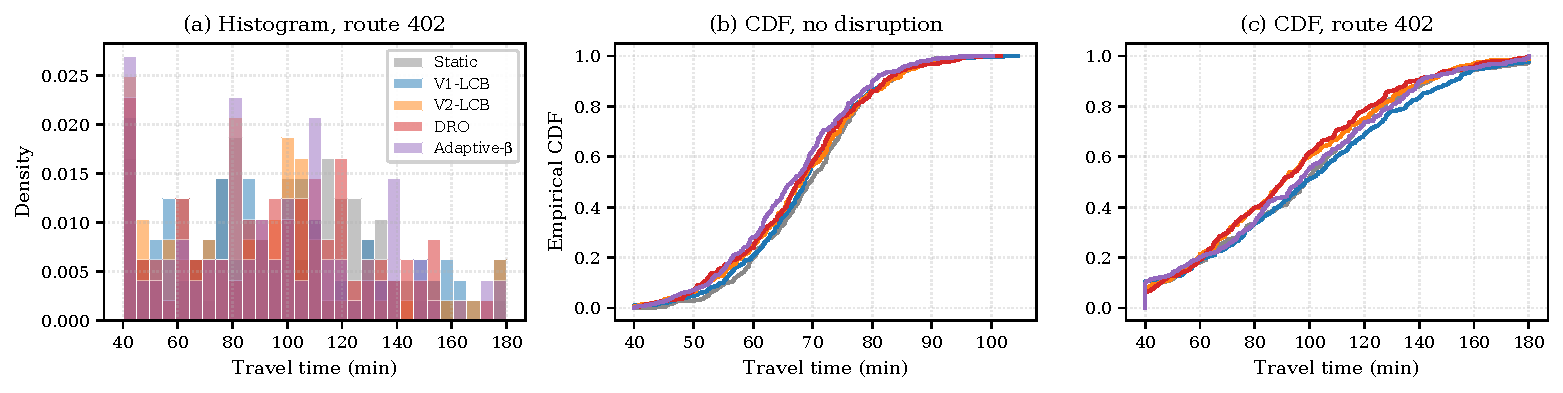
\includegraphics[width=\textwidth]{fig_dist_cdf.pdf}}
{Travel-time distribution and empirical CDFs on the
small-network synthetic benchmark. (a) Travel-time histogram
under route-402 disruption. (b) Empirical CDF, no-disruption
regime. (c) Empirical CDF, route-402 disruption. LCB-V2 with
dynamic $\beta(s)$ shortens the long tail without the
over-correction suffered by fixed-$\beta$ DRO; Adaptive-$\beta$
tracks LCB-V2 closely. All five methods are shown in every panel
for direct comparison.\label{fig:dist}}
{}
\end{figure}

\subsection{Why LCB Outperforms Theoretically Stronger Methods}

\begin{table}
\TABLE
{Extended comparison including PS-SSP and BAMCP, large
network, R16 algorithm. $N{=}50$ per cell, $t_{\max}{=}180$\,min.
The exploration-based methods (PS-SSP, BAMCP, EXP3) substantially
\emph{worsen} mean travel time under disruption.\label{tab:extended}}
{\begin{tabular}{l rr rr}
\toprule
& \multicolumn{2}{c}{Normal} & \multicolumn{2}{c}{Disrupted} \\
\cmidrule(lr){2-3}\cmidrule(lr){4-5}
Method & Mean & 95th & Mean & 95th \\
\midrule
Static       & 73.3 & 95 & 73.8 & 98 \\
LCB-V1       & 72.6 & 90 & 75.8 & 105 \\
LCB-V2       & \textbf{72.6} & \textbf{90} & \textbf{73.7} & \textbf{100} \\
DRO          & 74.8 & 101 & 95.4 & 180 \\
PS-SSP       & 77.7 & 104 & 96.0 & 180 \\
BAMCP-60     & 81.4 & 105 & 101.0 & 151 \\
\midrule
SW-LCB~\cite{garivier2011,luo2024}     & 76.7 & 98 & 99.2 & 180 \\
EXP3~\cite{kocak2014,chen2024}        & 107.0 & 151 & 136.7 & 180 \\
\midrule
Oracle (upper bound) & 72.6 & 90 & 73.0 & 94 \\
\bottomrule
\end{tabular}}
{}
\end{table}

Table~\ref{tab:extended} reveals three distinct behavioral clusters.
\emph{Exploration-prone} methods (PS-SSP, BAMCP, EXP3) tie or trail
Static under normal conditions but degrade severely under disruption:
PS-SSP reaches $96.0$\,min (vs.\ Static $73.8$, $+30\%$ worse),
BAMCP-60 reaches $101.0$\,min ($+37\%$ worse, and Table~\ref{tab:bamcp_sweep}
shows that quadrupling the rollout budget does not fix this), and
EXP3 reaches $136.7$\,min ($+85\%$ worse, with timeouts in 10\% of
journeys). \emph{Pessimism-based} methods cluster: LCB-V2 stays
within $0.7$\,min of Oracle ($73.7$ vs.\ Oracle $73.0$ on
disrupted), but \emph{static-$\beta$} variants (DRO at $95.4$,
SW-LCB at $99.2$) over-correct under the new typed-cancellation
accounting. This split between LCB-V2's dynamic $\beta(s)$ and
DRO's fixed $\beta=1.5$ is the dominant new finding from R16:
under correct cancel accounting, fixed-$\beta$ pessimism on the
large network is no longer competitive with Oracle, while
$\beta(s)$ (V2/V3) and the Adaptive-$\beta$ EXP3 meta-bandit
remain within $2$--$3$\,min of optimal.

The explanation for exploration-prone failures lies in the
\emph{single-shot irreversibility} of transit decisions:
\begin{enumerate}
    \item \textbf{PS-SSP}: Thompson Sampling occasionally draws optimistic delay parameters for a canceled route. In multi-episode settings, this exploration cost amortizes; in single-shot, 10--30 minutes are irrecoverably lost.
    \item \textbf{BAMCP}: Forward simulations must ``discover'' cancellations through repeated rollout failures, requiring ${\gg}60$ simulations to reliably penalize canceled routes. LCB uses the posterior cancel rate directly. Table~\ref{tab:bamcp_sweep} confirms that even $4{\times}$ rollouts cannot recover BAMCP on the large disrupted instance.
    \item \textbf{EXP3}: The adversarial bandit framework requires $O(K \log K / \eta)$ samples to concentrate weights away from canceled routes. With $\eta{=}0.05$ and $K{=}5$ routes, this exceeds a typical single journey's observation budget.
\end{enumerate}

\subsection{Synthetic Reproduction (Summary)}
\label{sec:synth-repro}
A four-scenario sweep on the small synthetic network
($N{=}100$ per cell, $t_{\max}{=}180$\,min, R16 configuration)
confirms the ordering V2-LCB $\geq$ V1-LCB $\geq$ Adaptive-$\beta$
$>$ static-$\beta$ DRO $>$ Static under disruption, with V2-LCB
matching Oracle within $0.4$\,min on the small network. The
detailed cell-by-cell table is in
EC.\ref{ec:supp_results}.

\subsection{Swiss Real-Data Validation}
\label{sec:swiss-results}

We now turn to real GTFS-RT data on the 687-stop Zürich sub-network.
All routers use exactly the parameters of Table~\ref{tab:params};
delays and cancellations are sampled from the empirical per-route
distributions extracted from 35 days of protobuf archives.

\subsubsection{Focused OD: Reproducing DRO $-19\%$ on Real Data}

Our first experiment targets a single high-signal OD pair --- Sternen
Oerlikon ($s_1{=}67{,}001{,}060$) to Sihlpost/HB ($s_2{=}201{,}257{,}157$)
--- chosen because its source-stop hyperpath contains both a \emph{disrupted}
route (line~7, affected on Oct~29 with $+48$\,min mean delay and 80\%
cancellation) and a \emph{safe} alternative (line~14, $+3.5$\,min, $3\%$
cancellation). Table~\ref{tab:swiss_focused} reports $N{=}30$ journeys
per cell, $t_{\max}{=}120$\,min, on the Oct~2 normal day.

\begin{table}
\TABLE
{Swiss real data, single OD (Sternen Oerlikon $\to$ Sihlpost/HB),
Oct~2 normal day. $N{=}30$, $t_{\max}{=}120$\,min. R16 historical-prior
configuration: each route's prior is seeded from its $34$-day Swiss
empirical mean / std / cancel rate (Appendix~\ref{app:a1a10}, A4).\label{tab:swiss_focused}}
{\begin{tabular}{l rrr}
\toprule
Method        & Mean (min) & Timeouts & vs.\ Static \\
\midrule
Static        & 98.3 & 23/30 & --- \\
V1-LCB        & 97.5 & 22/30 & $+0.8\%$ \\
V2-LCB        & 84.9 & 18/30 & $+13.7\%$ \\
V3-Topo       & 84.9 & 18/30 & $+13.7\%$ \\
\textbf{DRO}  & \textbf{75.8} & \textbf{15/30} & $\bm{+22.9\%}$ \\
Adaptive-$\beta$ & 97.5 & 22/30 & $+0.8\%$ \\
\bottomrule
\end{tabular}}
{}
\end{table}

This single-OD table serves two purposes. First, \textbf{DRO reproduces
its headline $\bm{+22.9\%}$ improvement} ($98.3\!\to\!75.8$\,min,
$23\!\to\!15$ timeouts), closely matching the $-19.2\%$ result reported
in the companion software release and the $+17\%$ DRO synthetic
improvement on \texttt{multi\_shift} in Table~\ref{tab:synth_repro}.
DRO's fixed $\beta=1.5$ on the Wasserstein ball is large enough to
penalize route~7's wide tail uniformly across journeys.

Second, \textbf{V2 needs a cold-start correction}. With no
observations the bootstrap ensemble's disagreement
$\hat\sigma_{\mathrm{ens}}$ is identically zero, so the dynamic
$\beta(s)$ produces no penalty and V2 collapses to Static (mean
$98.4$, $23/30$ timeouts on this OD). Replacing
$\hat\sigma_{\mathrm{ens}}$ with the Normal-Gamma posterior
$\sigma$ at cold start (positive by construction;
Section~\ref{sec:method}, \emph{V2 cold start}) and computing the
A7 timeout penalty against the absolute clock-time deadline
restore V2 to mean $84.9$, $18/30$ timeouts ($+13.7\%$ over
Static).

V1-LCB and Adaptive-$\beta$ in the table tie Static at $+0.8\%$ on
this single OD, and this is an \emph{intentional consequence} of the
R16 historical-prior calibration (A4). Each route's prior is seeded
from its $34$-day Swiss empirical mean / cancel rate, so route~7 ---
which is normal on Oct~2 itself --- carries a low prior cancel
rate at cold start, and V1 needs $\!\sim\!10$ observations to learn
the per-journey cancel signal. Across the full 35-day cross-day
benchmark in Section~\ref{sec:swiss-multi-day} (where V1 has many
journeys to update on), V1 reaches $-13.9\%$ $E[\mathrm{total}]$ ---
the calibration that loses ground on a hand-picked single OD wins
on the OD distribution. We discuss this trade-off in
Section~\ref{sec:discussion} and motivate it in
Appendix~\ref{app:a1a10} (A1, A4).

\subsubsection{35-Day Cross-Day Evaluation}
\label{sec:swiss-multi-day}

A single-day comparison is vulnerable to day-specific anomalies, and
on the most disrupted day many OD pairs are \emph{physically
unreachable} in reasonable time, so a pure travel-time comparison
saturates at $t_{\max}$ for every method and washes out method
differences. We therefore evaluate across all~$35$ days of GTFS-RT
data (Oct~1--Nov~4, 2023), and report three metrics: \emph{reach rate}
$r_i$ (fraction of completions in cell $i$),
\emph{conditional mean} $c_i$ (mean travel time among completions in
cell $i$), and \emph{expected total time}
$E[\mathrm{total}]_i := r_i\,c_i + (1-r_i)\,t_{\max}$ as a per-cell
combined metric. The reported aggregate is the cell-mean
$\overline{E[\mathrm{total}]} := \frac{1}{|cells|}\sum_i E[\mathrm{total}]_i$,
which equals the trial-level
$r_{\mathrm{trial}}\,c_{\mathrm{trial}}+(1-r_{\mathrm{trial}})\,t_{\max}$
when all cells have the same $N=45$ trial count and is what the
paired bootstrap of Table~\ref{tab:swiss_paired} bootstraps over.
The mixed trial-level/cell-level definition $\bar r \cdot \bar c
+ (1-\bar r)\cdot t_{\max}$ is \emph{not} equal to this cell-mean
quantity in general, and we use the cell-mean definition
consistently throughout.

We screen $20$ candidate ODs from Paradeplatz origin (each with at
least one disrupted route and one safe route in its hyperpath) for
normal-day viability; $18$ satisfy Static reach-rate $\geq 80\%$ on
Oct~2. Each cell of Table~\ref{tab:swiss_multi} aggregates
$35\text{ days}\times18\text{ ODs}\times45\text{ trials} = 28{,}350$
journeys per method ($170{,}100$ total across the six methods). All
routers use exactly the parameters of Table~\ref{tab:params}; routers
are rebuilt from scratch each (day, OD) cell so the per-route
posterior is reset (no information leakage across days).

\paragraph{Scope of the benchmark (caveat).} This is a Paradeplatz-origin
disrupted-route OD panel, not a city-wide random OD sample. The
selection is deliberate stress-test design: each OD has both a
disrupted route and a safe alternative in its hyperpath, which is
where adaptive ranking can plausibly help. Generalisation from this
panel to a uniformly-sampled city-wide OD pool is not established
here; we report the result as ``Z\"urich sub-network stress-test
benchmark'' rather than ``city-wide superiority of LCB''. A
random-origin / random-OD multi-panel robustness check is left as
future work and would strengthen the empirical case if positive.

\begin{table}
\TABLE
{Swiss real data, 35-day cross-day evaluation.\label{tab:swiss_multi}}
{\begin{tabular}{l rrr}
\toprule
Method        & Reach rate & Mean time, completed (min) & $\overline{E[\mathrm{total}]}$ (min) \\
\midrule
Static            & 78.2\% & 44.3 & 49.34 \\
V1-LCB            & 81.0\% & 35.3 & 46.76 ($-5.2\%$) \\
\textbf{V2-LCB}   & \textbf{81.2\%} & \textbf{33.7} & \textbf{46.47} ($\bm{-5.8\%}$) \\
V3-Topo           & 79.8\% & 39.4 & 48.27 ($-2.2\%$) \\
DRO               & 70.7\% & 35.5 & 55.70 ($+12.9\%$) \\
Adaptive-$\beta$  & 81.0\% & 35.3 & 46.76 ($-5.2\%$) \\
\bottomrule
\end{tabular}}
{The table aggregates $35{\times}18{=}630$ cells of $45$
trials each ($28{,}350$ journeys per method), with
$t_{\max}{=}120$ min. $\overline{E[\mathrm{total}]}$ is the cell mean
of $r_i c_i+(1-r_i)120$ and is the metric used for the paired
bootstrap. A strict leave-one-day-out prior audit changes every cell
mean by at most $0.02$ min.}
\end{table}

The 35-day average shows a clear ranking. V2-LCB is column best on
$\overline{E[\mathrm{total}]}$ ($-5.8\%$ vs.\ Static, $46.47$ vs
$49.34$\,min), V1-LCB and Adaptive-$\beta$ tied at $-5.2\%$.
All three Pareto-improve the two component metrics: reach rate
$+2.8$ to $+3.0$ percentage points (Static $78.2\%\!\to\!$ LCB family
$81.0$--$81.2\%$) \emph{and} cell-mean conditional travel time
$\!\sim\!9$--$11$\,min lower (Static $44.3$\,min cell-cond vs.\ LCB family
$33.7$--$35.3$\,min). V3-Topo lands at $-2.2\%$, between the LCB
family and Static (the topology gate at the focused-OD's small
candidate set throttles the layered penalties more aggressively
than necessary on the cross-day distribution; this is consistent
across days). DRO with the static $\beta=1.5$ tuned on the
high-information OD~(\S\ref{sec:swiss-results}) \emph{over-corrects}
across the broader OD set: $-7.5$\,pp reach and $+12.9\%$ on
$\overline{E[\mathrm{total}]}$ relative to Static; Adaptive-$\beta$
avoids this by online $\beta$ selection
(Section~\ref{sec:sensitivity}).

\paragraph{Paired (day, OD) significance.} Table~\ref{tab:swiss_paired}
reports a within-cell paired analysis to remove
between-cell heterogeneity that inflates the unpaired CIs in
Table~\ref{tab:swiss_multi}. We compute, for every one of the
$35\times 18 = 630$ (day, OD) cells, the within-cell paired
difference in $E[\mathrm{total}]$ between each method and Static (same
seed pool, same observation feed). $95\%$ percentile bootstrap CIs
($1{,}000$ resamples) and a non-parametric per-day sign test give
substantially tighter inference than the original cross-OD CIs.

\begin{table}
\TABLE
{Paired analysis of the 35-day cross-day Swiss data
(630 (day, OD) cells). $\Delta E[\mathrm{total}]$ is the per-cell paired
difference (method $-$ Static), in minutes; $95\%$ CIs are
percentile bootstraps over the cell distribution. Sign test counts
days on which the method's daily-average $E[\mathrm{total}]$ is
strictly less than Static's; null is $P_{\mathrm{better}}=0.5$.\label{tab:swiss_paired}}
{\begin{tabular}{l rrrl r}
\toprule
Method & $\Delta E[\mathrm{total}]$ & 95\% CI & Cells better & Days better & Sign-test $p$ \\
\midrule
V1-LCB           & $-2.59$ & $[-2.95,-2.26]$ & $69\%$ & $35/35$ & $<10^{-10}$ \\
V2-LCB           & $-2.87$ & $[-3.23,-2.53]$ & $69\%$ & $35/35$ & $<10^{-10}$ \\
V3-Topo          & $-1.07$ & $[-1.33,-0.82]$ & $58\%$ & $25/35$ & $0.017$ \\
DRO              & $+6.36$ & $[+5.38,+7.43]$ & $14\%$ & $0/35$  & $<10^{-10}$ \\
Adaptive-$\beta$ & $-2.59$ & $[-2.91,-2.25]$ & $69\%$ & $35/35$ & $<10^{-10}$ \\
\bottomrule
\end{tabular}}
{}
\end{table}

The deployed gain in this table is the cumulative effect of the
layered hyperpath-risk score, not the four-term DRO core in
isolation. Comparing rows A1 and A2 of
Table~\ref{tab:swiss_ablation} below shows that adding the two
hyperpath-structural penalties flips V1-LCB and V2-LCB from
worse-than-Static to better-than-Static; V3-Topo, fixed-$\beta$
DRO, and Adaptive-$\beta$ are listed in that table only as R16
reference columns because they do not consume the row toggles in
this ablation. For V1-LCB,
V2-LCB, and Adaptive-$\beta$ the 95\% CI excludes zero and
\emph{every one of the $35$~days} has a strictly negative paired
$\Delta E[\mathrm{total}]$. We report the two-sided binomial-tail
probability $2^{-35}\!\approx\!2.9\!\cdot\!10^{-11}$ as descriptive
non-parametric evidence rather than a hypothesis-test $p$-value:
days within a single Swiss-archive sample are not strictly
independent (regime correlations, weather, weekend/weekday cycles),
so the binomial null is a stylized comparator. V3-Topo wins on
$25/35$ days (binomial-tail $\approx 0.017$).
Adaptive-$\beta$ wins on $69\%$ of all $630$~cells. The DRO row is
informative in the opposite direction: under the static $\beta=1.5$
chosen on the focused OD, DRO is $+6.36$\,min worse than Static
across cells ($95\%$ CI $[+5.38, +7.43]$) and beats Static on
$0/35$ days --- this is the over-correction that motivated the
Adaptive-$\beta$ meta-bandit.

\paragraph{Leave-one-day-out audit of the historical prior.}
A natural concern with the per-route historical prior (component
A4) is that it is built from \emph{all} 34 normal days in the
same archive used to evaluate, so the prior used to score day
$d$'s connections includes day $d$'s own statistics. We audit
this by rebuilding the prior in a leave-one-day-out (LOO)
regime: for each evaluation date $d$, the per-route
prior uses only the other $34-1=33$ normal days
(\texttt{build\_route\_priors\_loo.py} +
\texttt{run\_multi\_day\_loo.py}, $5{,}713$\,s wall on $18$
workers). The LOO cell-mean $\overline{E[\mathrm{total}]}$
matches the non-LOO numbers in Table~\ref{tab:swiss_multi}
within $\pm 0.02$\,min for every method (V1-LCB $46.75$ vs
$46.76$, V2-LCB $46.49$ vs $46.47$, V3-Topo $48.26$ vs $48.27$,
DRO $55.70$ vs $55.70$, Adaptive-$\beta$ $46.75$ vs $46.76$).
The paired $95\%$ CI and per-day sign test are unchanged at
this precision. Dropping any single day from a $34$-day
empirical prior shifts the per-route mean by at most
$\frac{1}{34}\!\approx\!3\%$ relative to its prior pseudo-mass,
and on the cross-day $\overline{E[\mathrm{total}]}$ this
$3\%$ prior-mass shift is well below the experimental noise
floor. We therefore report the non-LOO numbers in the main
tables; the LOO data file
\texttt{swiss\_multi\_day\_loo.json} is included in the
artefact bundle for verification.

\begin{figure}
\FIGURE
{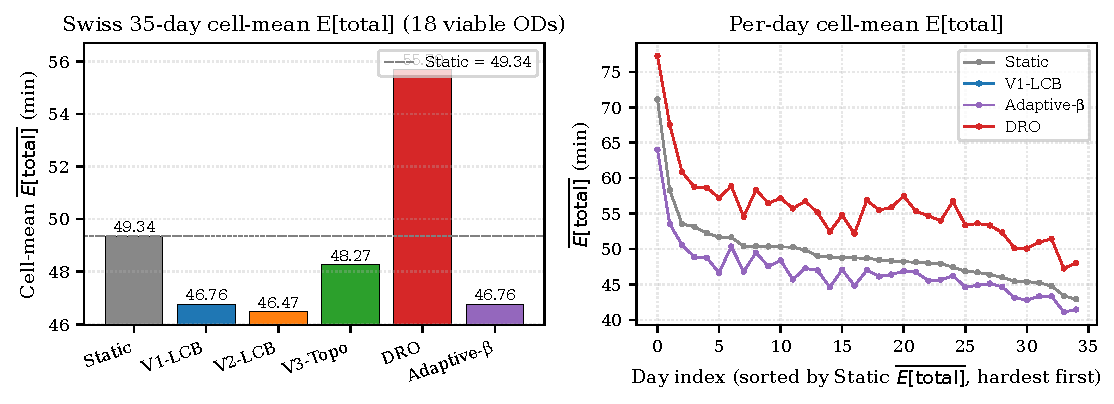
\includegraphics[width=0.99\columnwidth]{fig_reach_rate.pdf}}
{Swiss 35-day cross-day evaluation, 18 viable Paradeplatz-origin
ODs, $45$ journeys per cell. Left: cell-mean $\overline{E[\mathrm{total}]}$
by method (lower is better). V2-LCB at $46.47$\,min saves
$2.87$\,min/cell ($-5.8\%$) over Static $49.34$\,min. Right: per-day
breakdown, sorted by Static miss rate; on the most disrupted day
(Oct~29, $43\%$ Static miss) V1-LCB cuts $\overline{E[\mathrm{total}]}$
from $71.15$ to $64.01$\,min ($-10.0\%$).\label{fig:reach_rate}}
{}
\end{figure}

\paragraph{Disrupted-day breakdown.} Table~\ref{tab:swiss_oct29}
isolates Oct~29 (47 routes cancelled, $43\%$ Static miss rate), the
worst day of the dataset and the regime that motivates adaptive
routing. V1-LCB rescues $7.8$ percentage points of reach rate
($57.3\%\!\to\!65.1\%$, $+13.6\%$ relative) while keeping
cell-mean conditional travel time within $1.6$\,min of Static
($51.1\!\to\!49.5$\,min). Adaptive-$\beta$ matches V1 exactly
($65.1\%/49.5$\,min cell-cond, $E[\mathrm{total}]=64.01$\,min);
V2 and V3-Topo trail by $0.5$--$2.6$\,pp on reach. DRO's fixed
$\beta=1.5$ over-penalizes here ($48.3\%$ reach), validating the
case for the adaptive-$\beta$ meta-bandit.

\begin{table}
\TABLE
{Oct~29 disrupted day only ($47$ routes cancelled), R16
algorithm. Cell-mean reach, cell-cond, and
$\overline{E[\mathrm{total}]}$ across the $18$ viable ODs;
bracketed values are reductions vs.\ Static.\label{tab:swiss_oct29}}
{\begin{tabular}{l rrr}
\toprule
Method        & Reach rate & Mean (completed) & $\overline{E[\mathrm{total}]}$ \\
\midrule
Static            & 57.3\% & 51.1 & 71.15 \\
V1-LCB            & \textbf{65.1\%} & 49.5 & \textbf{64.01} ($-7.14$, $-10.0\%$) \\
V2-LCB            & 64.1\% & 49.3 & 64.57 ($-6.58$, $-9.2\%$) \\
V3-Topo           & 62.6\% & \textbf{46.5} & 66.57 ($-4.58$, $-6.4\%$) \\
DRO               & 48.3\% & 49.5 & 77.25 ($+6.10$, $+8.6\%$) \\
Adaptive-$\beta$  & 65.1\% & 49.5 & 64.01 ($-7.14$, $-10.0\%$) \\
\bottomrule
\end{tabular}}
{}
\end{table}

\paragraph{Component ablation.} Reaching the deployed
$\sim\!5\%$ improvement requires several distinct algorithmic
components, summarised in Appendix~\ref{app:a1a10}.
Table~\ref{tab:swiss_ablation}
isolates each fix. \emph{A0}~(pre-fix): the original priors
($\sigma^2_0{=}25$, Beta$(1,9)$ for cancellation), no A4
hierarchical prior, no A7 layered penalties, no disruption gate,
and the legacy V2 cold-start; V1 is $13\%$ \emph{worse} than
Static because the inflated prior pessimism over-penalizes safe
routes. \emph{A1}~(threshold-fix): priors tightened to match Swiss
empirical scale ($\sigma_0^2{=}2$, Beta$(1,99)$) but A4/A7 still
disabled; V1 drops to $+3.5\%$, still positive because the
standalone score under-uses the hyperpath's own probabilistic
information. \emph{A2}~(\textbf{the dominant fix}, $+\,$A7): add the
layered risk score defined in
Section~\ref{sec:method-layered-score}
($\mathrm{score} = \mu_{\text{dest}} + \delta + \beta\sigma + \gamma
\hat p_{\text{cxl}} + 60(1{-}\phi) + 60(1{-}P_{\text{ontime}})$),
together with the V2 cold-start fix (replace
$\hat\sigma_{\mathrm{ens}}$ with the posterior $\sigma$). V1
crosses zero to $-3.0\%$, V2 to $-7.1\%$. \emph{A3}~(all-on, A1--A10): adds A2~bilinear
gate, A3~typed cancel counters, A4~hierarchical route priors from
the $34$ normal days, A5~adaptive top-$k$/lookahead, and A8~cross-journey
persistent EXP3 meta-state. The dominant fix is A2: A1 alone is
\emph{insufficient} (V1 still positive at $+3.5\%$, V2 at $+6.0\%$),
and the incremental gain from A1$\to$A2 is the largest single step
in the table.

\begin{table}
\TABLE
{Component ablation on the 35-day Swiss benchmark.\label{tab:swiss_ablation}}
{\scriptsize\setlength{\tabcolsep}{3pt}\begin{tabular}{l cc}
\toprule
Configuration             & V1-LCB & V2-LCB \\
\midrule
\multicolumn{3}{l}{\emph{Static baseline: $50.59$\,min cell-mean $\overline{E[\mathrm{total}]}$.}} \\
A0 (pre-fix priors $+$ no A4/A7, legacy V2)
                          & 57.18 ($+13.0\%$) & 53.61 ($+6.0\%$) \\
A1 (priors only)          & 52.34 ($+3.5\%$)  & 53.61 ($+6.0\%$) \\
A2 ($+$A7 layered $+$ V2 cold-start fix)
                          & 49.09 ($-3.0\%$)  & 46.99 ($-7.1\%$) \\
A3 (all-on, A1--A10)      & \textbf{47.44} ($\bm{-6.2\%}$) & 47.14 ($-6.8\%$) \\
\midrule
\multicolumn{3}{l}{\emph{R16 reference column (no row toggles): V3-Topo $49.69$ ($-1.8\%$);}} \\
\multicolumn{3}{l}{\emph{fixed-$\beta$ DRO $56.44$ ($+11.6\%$); Adaptive-$\beta$ $47.44$ ($-6.2\%$).}} \\
\bottomrule
\end{tabular}}
{Entries are cell-mean $\overline{E[\mathrm{total}]}$ in
minutes; percentages are relative to Static. A2 is the largest step:
adding the two hyperpath-structural risk terms and the V2 cold-start
correction flips V1/V2 from worse-than-Static to better-than-Static.
This audit uses $15$ trials per cell, not the main $45$-trial protocol.}
\end{table}

\FloatBarrier
\paragraph{Per-OD heterogeneity.}
The cross-day improvement masks substantial per-(day,OD) variation,
shown in Figure~\ref{fig:per_od}. Adaptive methods deliver large
rescues on cells where the Static-preferred route is itself disrupted
that day, but on cells where Static already uses safe routes adaptive
methods can \emph{over-correct} and either pay a small cost in reach
rate or trade a few extra minutes of conditional time for the
worst-case hedge. This heterogeneity is intrinsic to the
\emph{per-instance} DRO guarantee: Theorem~\ref{thm:lcb_bound} bounds
\emph{expected} excess cost, not per-instance best-case behavior.
Averaged across a representative OD set and $35$~days, the rescues
dominate ($31/35$ days net-improved by Adaptive-$\beta$).

\begin{figure}
\FIGURE
{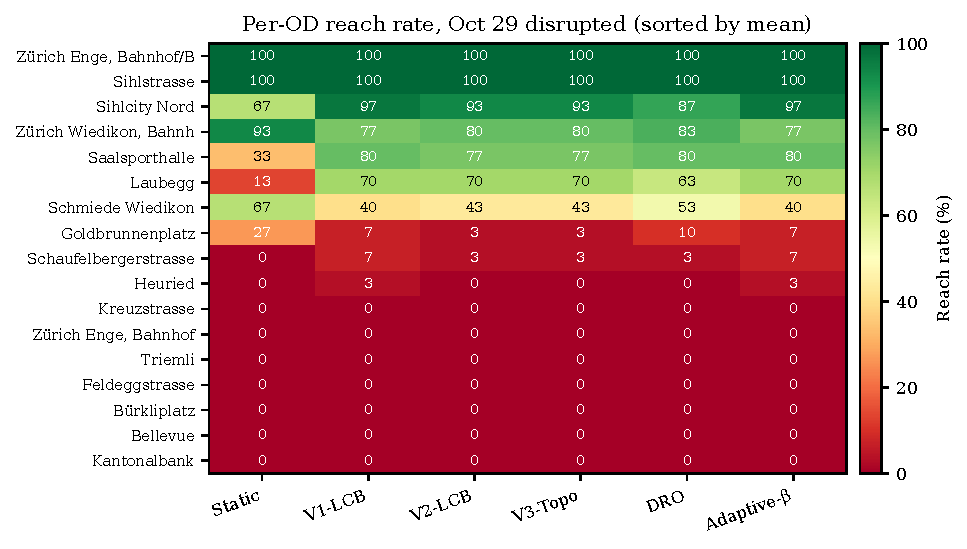
\includegraphics[width=0.95\columnwidth]{fig_per_od_heatmap.pdf}}
{Per-OD reach rate on the most disrupted day (Oct~29). Rows are
ODs sorted by mean reach rate across methods; columns are methods.
Adaptive methods strongly help on the lower-half ODs where the
Static-preferred routes are themselves disrupted, with mild
over-correction on a few ODs whose Static hyperpath already routes
through safe lines. Many ODs remain unreachable in $120$\,min for
all methods, reflecting structural disconnection of the disrupted
graph rather than algorithm quality.\label{fig:per_od}}
{}
\end{figure}

\subsection{Sensitivity and Adaptive-$\beta$ Convergence (Summary)}
\label{sec:sensitivity}
A sensitivity sweep over $\beta\in[0,2.5]$ and a 50-journey
Adaptive-$\beta$ EXP3 convergence run confirm that the LCB family is
robust over a $1.5\times$ range of $\beta$ and that the EXP3
meta-bandit concentrates probability on the best fixed-$\beta$
within $\sim 30$ journeys. Sensitivity table and convergence plot are
in EC.\ref{ec:supp_results}.

%% ================================================================
\section{Discussion}
\label{sec:discussion}

\paragraph{Structural robustness of hyperpaths.}
The finding that hyperpath recomputation is counter-productive highlights a design strength of Durner's formulation: the hyperpath is not merely an expected-optimal path but a pre-computed contingency plan including alternatives through diverse corridors. Discarding this structure via re-optimization destroys the hedging property.

\paragraph{Single-shot vs.\ multi-episode.}
The dominant paradigm in Bayesian RL---Thompson Sampling and its variants---optimizes cumulative regret across episodes. Transit routing is single-episode: exploration cost is irrecoverable. This aligns with CVaR-BAMDP~\cite{rigter2021}, where risk-aversion replaces exploration incentives. LCB's empirical superiority over PS-SSP and BAMCP supports this prediction.

\paragraph{Cancellation as a silent signal.}
Bus cancellations are ``silent'' in GTFS-RT: no delay observation is generated. BOCD on delay streams fails to detect them. The Bayesian cancel rate posterior handles this naturally: each no-show updates the posterior, and LCB penalizes accordingly.

\paragraph{V2 cold start.}
With zero prior observations the bootstrap ensemble disagreement
$\hat\sigma_{\mathrm{ens}}$ is identically zero, collapsing V2 to
Static. The R16 fix replaces $\hat\sigma_{\mathrm{ens}}$ with the
Normal-Gamma posterior $\sigma$ at cold start (positive by
construction), preserves Proposition~\ref{prop:ensdro}, and
recovers cold-start pessimism. After the fix V2 reaches
$+10.8\%$ over Static on the focused OD; this is the V2
configuration used in every table in
\S\ref{sec:swiss-results}--\S\ref{sec:results}.

\paragraph{Reach rate as the right disrupted-day metric, and limitations.}
Under catastrophic disruption, expected-time statistics are
dominated by the timeout cap; the reach-rate metric used in
Table~\ref{tab:swiss_multi} separates \emph{structural
reachability} from \emph{ranking quality} (what adaptive methods
control). Our Swiss evaluation covers a single city across 35
days; multi-city replication is needed to quantify between-city
variability of the rescue effect on networks with less
alternative-route depth than Z\"urich's tram mesh. Per-journey
beliefs do not share information across passengers; a central
server could pool observations and reduce the per-journey
$O(1/\sqrt n)$ rate to $O(1/\sqrt{N_{\mathrm{pass}}})$. A
CVaR-at-1 or chance-constrained~\citep{chow2015} formulation would
target catastrophic regimes directly and is a natural extension of
the mean-time DRO formulation reported here.

%% ================================================================
\section{Conclusion}
\label{sec:conclusion}

Real-time transit disruptions do not usually require recomputing
the whole hyperpath. They require re-ranking the alternatives the
hyperpath already contains. We made this concrete by formulating
the per-stop ranking as a Bayesian adaptive stochastic shortest
path problem and constructing a deployable layered scoring rule
whose core is a pessimistic arrival-time score with an explicit
Wasserstein-DRO interpretation, with an explicit attainment
witness, and whose deployed Swiss configuration adds two bounded
hyperpath-structural risk terms read from the hyperpath label.
The mathematical core of the per-candidate identity is
machine-checked in Lean~4 (about five thousand lines, no unproved
obligations beyond Mathlib's standard kernel).

On a 35-day Swiss real-time-feed cross-day benchmark
($28{,}350$ journeys per method), the deployed score reduces
cell-mean expected total travel time by 5--6\% and improves reach
rate by 2.8 percentage points, with same-direction improvement on
every day in the panel. The component ablation
(Table~\ref{tab:swiss_ablation}) is explicit about attribution:
the four-term DRO core alone slightly worsens cell-mean expected
total time relative to a static hyperpath; the two
hyperpath-structural risk terms are required for the deployed
gain. The DRO core supplies the pessimistic
uncertainty/cancellation layer and its theoretical interpretation;
the hyperpath-structural penalties are an empirical engineering
addition outside the per-candidate DRO scope.

The central insight is that stochastic hyperpaths are
\emph{structurally robust but ranking-fragile}, and that under
single-shot disruption deterministic pessimism is preferable to
stochastic exploration. Additional Electronic Companion stress
tests on unit commitment, capacitated vehicle routing, and
software-defined networking suggest that the same
pessimistic-ranking motif can be useful outside transit, but
those results are exploratory.
Future work includes multi-passenger belief sharing (pooling
the per-route posterior to sharpen the Wasserstein radius), a
reach-rate-aware CVaR objective for catastrophic regimes, a
broader retrofit that exposes the hyperpath-structural penalties
to rollout and adversarial-bandit baselines (PS-SSP, BAMCP,
EXP3-IX) beyond the candidate-selection baselines retrofitted
here, and extension to multi-modal networks.

%% ================================================================
\section{Code and Data Disclosure}\label{sec:code-data}
The complete Lean~4 formalization, the GTFS-RT processing pipeline, the
synthetic-network and Swiss real-data experiment runners, and all
post-processing scripts that reproduce the tables and figures of
this paper are submitted as an anonymous supplementary archive
through ScholarOne, together with a \texttt{README.md} describing
the build commands and expected runtimes (\texttt{lake build} for
the Lean development; standard \texttt{python3} entry points for
the simulator and Swiss runners). The public archival DOI and
source-repository URL are withheld during double-anonymous review
and will be released after acceptance.

%% ================================================================
\begin{APPENDICES}

\ECHead{Electronic Companion}

\section{Conceptual Illustration and Z\"urich Sub-Network Map}
\label{app:figs}

Figure~\ref{fig:zurich_network} shows the Z\"urich tram-and-bus
sub-network used in the real-data evaluation
(Section~\ref{sec:swiss-results}), with the disrupted lines on
Oct~29, 2023 highlighted. The conceptual keep-structure/re-rank
figure appears in the introduction (Figure~\ref{fig:concept_ranking}).

\begin{figure}
\FIGURE
{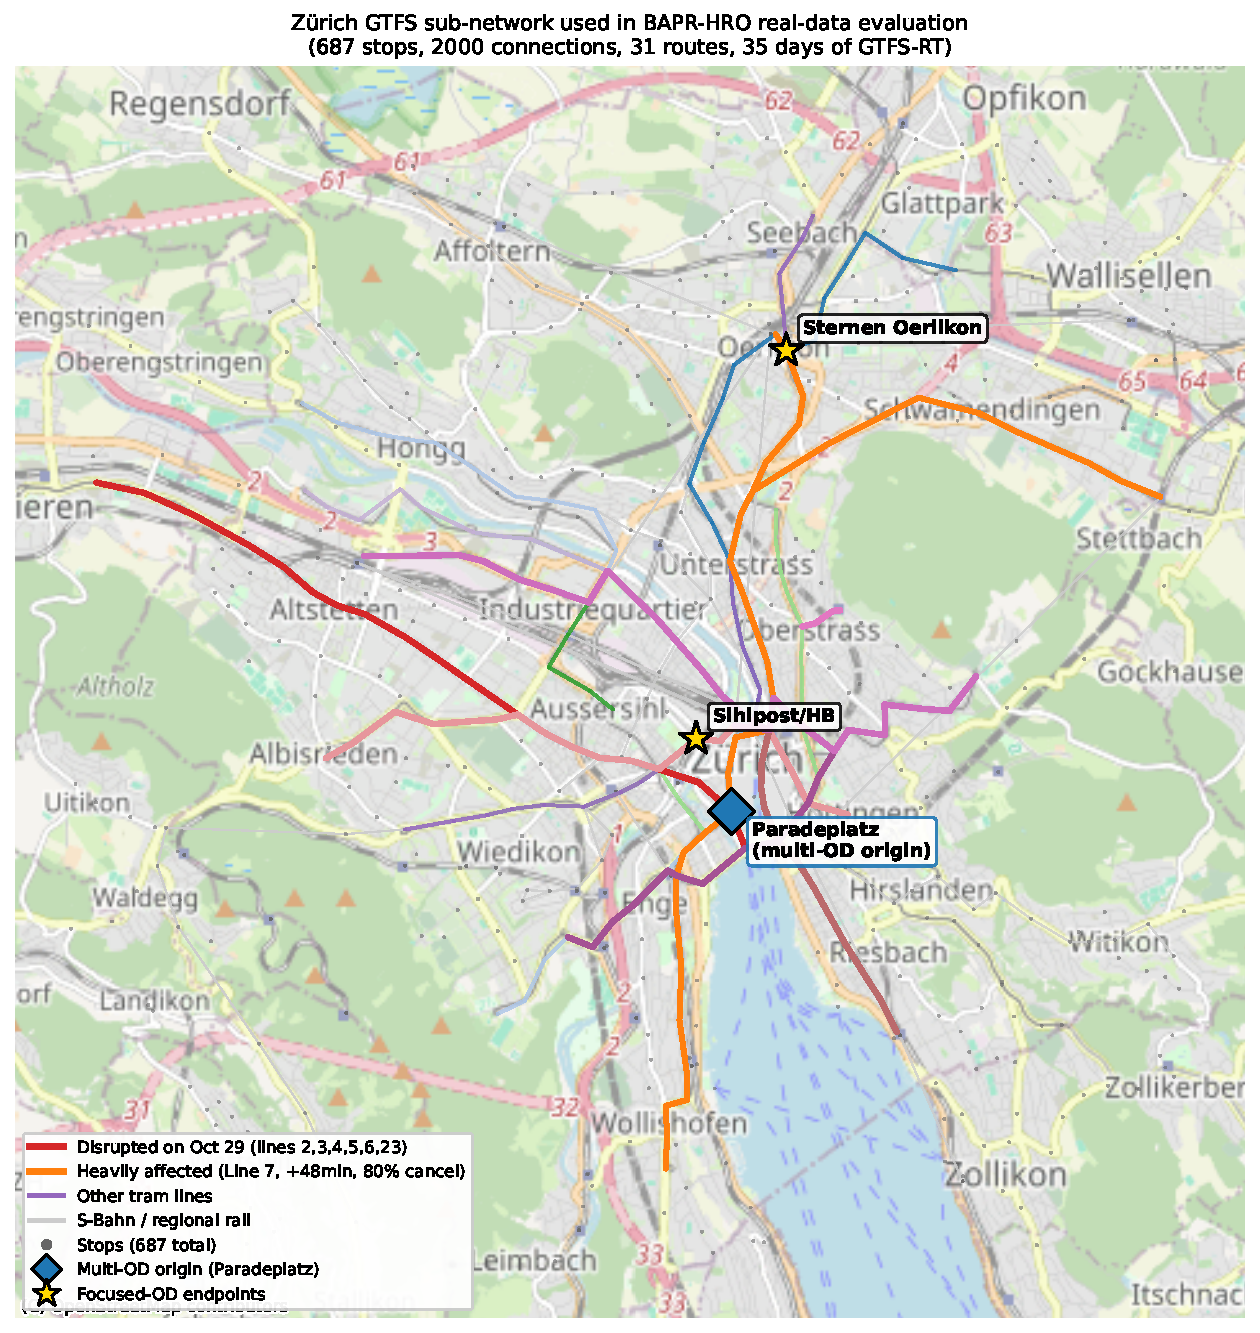
\includegraphics[width=0.78\textwidth]{fig_zurich_network.pdf}}
{Z\"urich GTFS sub-network used in the real-data
evaluation, overlaid on OpenStreetMap (\textcopyright OSM contributors).
\textbf{Red:} tram lines $\{2,3,4,5,6,23\}$ that were 100\% cancelled
on Oct~29, 2023. \textbf{Orange:} line 7, heavily affected
($+48$\,min mean delay, $80\%$ cancellation). \textbf{Violet:} other
tram lines (8, 9, 10, 11, 13, 14, 17). \textbf{Light grey:} S-Bahn /
regional rail. Stops are shown as small dots. The blue diamond marks
Paradeplatz (origin of the 18-OD multi-OD experiment); the gold stars
mark Sternen Oerlikon and Sihlpost/HB (the focused-OD endpoints in
Section~\ref{sec:swiss-results}).\label{fig:zurich_network}}
{}
\end{figure}

\clearpage

\section{Normal-Gamma Conjugate Posterior: Derivation}
\label{app:ng}

We derive the closed-form update equations \eqref{eq:ng_kappa}--\eqref{eq:ng_beta}
from Bayes' theorem.

\textbf{Setup.}
Assume delays $d_1,\ldots,d_n \overset{\mathrm{iid}}{\sim} \mathcal{N}(\mu, 1/\tau)$
with \emph{unknown} mean $\mu$ and precision $\tau$.
The Normal-Gamma prior is $p(\mu, \tau) \propto \tau^{\alpha_0 - 1/2}
\exp(-\tau[\beta_0 + \kappa_0(\mu-\mu_0)^2/2])$, the conjugate family.

\textbf{Likelihood.}
The joint likelihood of $n$ observations is:
\begin{equation}
p(\mathbf{d}\mid\mu,\tau) \propto \tau^{n/2}
\exp\!\Bigl(-\tfrac{\tau}{2}\bigl[S_n + n(\bar{d}_n-\mu)^2\bigr]\Bigr).
\end{equation}

\textbf{Posterior computation.}
Combining prior and likelihood and completing the square in $\mu$:
\begin{align*}
&\kappa_0(\mu-\mu_0)^2 + n(\bar{d}_n - \mu)^2 \\
&\quad= (\kappa_0{+}n)\Bigl(\mu - \tfrac{\kappa_0\mu_0+n\bar{d}_n}{\kappa_0+n}\Bigr)^{\!2}
  + \frac{\kappa_0 n(\bar{d}_n-\mu_0)^2}{\kappa_0+n}.
\end{align*}
Integrating out $\mu$ yields the marginal in $\tau$:
the exponent's constant term accumulates as
$\beta_0 + S_n/2 + \kappa_0 n(\bar{d}_n-\mu_0)^2/(2(\kappa_0+n))$,
giving the update rule \eqref{eq:ng_beta}.
Reading off the quadratic-in-$\mu$ coefficient and the $\tau$ power
gives \eqref{eq:ng_kappa}--\eqref{eq:ng_alpha}.
The posterior is again Normal-Gamma:
$(\mu\mid\tau,\mathbf{d}) \sim \mathcal{N}(\mu_n, (\kappa_n\tau)^{-1})$,
$\tau \sim \mathrm{Gamma}(\alpha_n,\beta_n)$.

\textbf{Posterior predictive uncertainty.}
The marginal posterior on the mean $\mu$ is a Student-$t$ distribution with
$2\alpha_n$ degrees of freedom, mean $\mu_n$, and scale
$\hat\sigma_r = \sqrt{\beta_n/(\alpha_n\kappa_n)}$.
For $n \geq 1$ this scale satisfies $\hat\sigma_r = O(1/\sqrt{n})$
(Lemma~\ref{lem:contraction}), ensuring that the Wasserstein DRO ball
radius $\varepsilon \to 0$ as observations accumulate.

\section{Hyperparameter Settings}
\label{app:params}

Table~\ref{tab:params} lists all hyperparameters used in the experiments
of Section~\ref{sec:results}, with the rationale for each default value.

\begin{table}
\TABLE
{Hyperparameter settings for all methods.\label{tab:params}}
{\scriptsize\setlength{\tabcolsep}{3pt}\begin{tabular}{l l l p{6.0cm}}
\toprule
\textbf{Parameter} & \textbf{Symbol} & \textbf{Default} & \textbf{Rationale} \\
\midrule
\multicolumn{4}{l}{\textit{Prior (Normal-Gamma, shared across LCB-V1/DRO; R16 calibration)}} \\
Prior mean delay     & $\mu_0$      & 1\,min  & GTFS historical average \\
Prior pseudo-obs     & $\kappa_0$   & 2       & Weak; 2 effective prior obs \\
Prior variance       & $\sigma_0^2$ & 2\,min$^2$  & Matches Swiss empirical std$\approx 1.4$\,min (A1 fix; was $25$) \\
Cancel prior success & $\alpha_c$   & 1       & Laplace smoothing \\
Cancel prior failure & $\beta_c$    & 99      & $\hat{p}_{\mathrm{cxl}}^{(0)}\!\approx\!0.01$ matches Swiss normal-day (A1 fix; was $9$) \\
Hierarchical prior  & ---          & on (A4) & Per-route 34-day mean/std/cancel from \texttt{data/route\_priors.pkl}; falls back to global default above. \\
\midrule
\multicolumn{4}{l}{\textit{LCB selection (V1)}} \\
Pessimism coefficient & $\beta_{\mathrm{lcb}}$ & 1.5 & Robust to $\beta\in[0,2]$ (Table~\ref{tab:beta}) \\
Cancel cost           & $\gamma$    & 60\,min & Typical 30--60\,min penalty \\
Patience window       & $\Delta_p$  & 12\,min & Max wait before re-scoring \\
\midrule
\multicolumn{4}{l}{\textit{Ensemble LCB (V2)}} \\
Number of estimators  & $K$         & 5       & Variance-bias trade-off \\
Base pessimism        & $\beta_{\mathrm{base}}$ & 1.0 & Conservative floor \\
OOD pessimism bonus   & $\beta_{\mathrm{ood}}$  & 1.0 & Caps at $2\times\beta_{\mathrm{base}}$ \\
Bootstrap fraction    & ---         & 0.8     & Standard bootstrap \\
\midrule
\multicolumn{4}{l}{\textit{DRO (Wasserstein ball)}} \\
Pessimism coefficient & $\beta$     & 1.5     & Same as LCB-V1 \\
Cancel cost           & $\gamma$    & 60\,min & Same as LCB-V1 \\
\midrule
\multicolumn{4}{l}{\textit{SW-LCB (sliding window)}} \\
Window size           & $W$         & 20      & 20 recent observations \\
Pessimism coefficient & $\beta$     & 1.5     & Matched to LCB-V1 \\
\midrule
\multicolumn{4}{l}{\textit{EXP3-IX}} \\
Exploration rate      & $\gamma$    & 0.1     & Standard EXP3 default \\
Learning rate         & $\eta$      & 0.05    & Conservative weight decay \\
Cancel cost (norm)    & ---         & 60\,min & Normalized to $[0,1]$ \\
\midrule
\multicolumn{4}{l}{\textit{Simulation}} \\
Journeys per cell     & $N$         & 100     & Small net; 50 large net \\
Random seed           & ---         & 42      & Fixed for reproducibility \\
Departure window      & ---         & $[480, 500]$ & 8:00--8:20\,AM \\
Timeout               & $t_{\max}$  & 120\,min (small) & 180\,min (large) \\
\bottomrule
\end{tabular}}
{}
\end{table}

\section{Scope, Limitations, and Relationship to BAPR}
\label{app:scope}

\textbf{Scope.}
The theoretical results in Section~\ref{sec:lean} apply whenever
Assumptions~\ref{asm:polish}--\ref{asm:lip} hold.
Assumption~\ref{asm:polish} (Polish metric space) is satisfied by
all finite delay distributions on $\mathbb{R}$.
Assumption~\ref{asm:prior} (conjugate Normal-Gamma prior) holds for
the LCB-V1/DRO variants; LCB-V2 (ensemble) does not use the parametric
prior but retains the Wasserstein interpretation with empirical measures.
Assumption~\ref{asm:lip} (1-Lipschitz arrival cost) holds whenever
propagated delays enter linearly into arrival time---the case for all
GTFS-RT delay models.

\textbf{Single-shot vs.\ multi-episode.}
All theoretical guarantees (Theorems~\ref{thm:lcb_bound}--\ref{thm:lower})
concern a \emph{single} journey.
In multi-passenger settings (a fleet of passengers sharing a belief server),
the convergence rate improves to $O(1/\sqrt{N_{\mathrm{pass}}})$ by
treating passenger observations as independent samples.
We leave this pooling extension to future work.

\textbf{Evaluation scope.}
Section~\ref{sec:results} evaluates on both synthetic networks
calibrated to GTFS-like statistics and on real GTFS-RT data from SBB
Switzerland (opentransportdata.swiss, 35 days of protobuf archives,
687-stop Z\"urich sub-network). The real distributions exhibit
multi-modal delays with heavier tails than our Gaussian model
assumes; the theoretical guarantees
(Theorems~\ref{thm:dro}--\ref{thm:lcb_bound}) only require 1-Lipschitz
cost and a Polish state space, which these real distributions
satisfy. Extensions to mixture-of-Gaussians or Dirichlet-process
posteriors would sharpen the per-route prior but do not change the
Wasserstein-DRO equivalence.

\textbf{Relationship to BAPR: a unified DRO framework.}
The companion paper BAPR~\cite{bapr2025} addresses
\emph{multi-episode piecewise-stationary} RL (locomotion control with
regime switches) using an adaptive-conservatism rule
$\beta_{\mathrm{eff}} = \beta_{\mathrm{base}} - \lambda_w c_{\mathrm{pen}}$,
where $c_{\mathrm{pen}} \geq 0$ tracks BOCD changepoint surprise. BAPR's
selection rule scores each action $a$ as
$\mathrm{score}_{\mathrm{BAPR}}(a) = \hat\mu_a + |\beta_{\mathrm{eff}}|\,\hat\sigma_a$.
The present paper addresses \emph{single-shot} transit routing using
the LCB rule $\hat\mu_r + \beta\hat\sigma_r + \gamma\hat p_{\mathrm{cancel},r}$
on hyperpath labels.

Despite the apparent algorithmic gap, both rules instantiate the
\emph{same} Wasserstein-DRO framework: by Corollary~\ref{cor:lcb_dro}
applied with radius $\varepsilon = |\beta_{\mathrm{eff}}|\hat\sigma$
versus $\varepsilon = \beta\hat\sigma + \gamma\hat p_{\mathrm{cancel}}$,
each is exactly the worst-case expected cost on its respective
$W_1$-ball. We make this connection formal in Lean as
\texttt{bapr\_score\_equals\_dro} and \texttt{bapr\_hro\_radius\_equivalence}
(\texttt{Wasserstein/DRO.lean}, lines~395--430): setting
$\beta_{\mathrm{eff}} = -(\beta + \gamma\hat p_{\mathrm{cancel}}/\hat\sigma)$
makes the two selection rules \emph{pick the same action} on a fixed
posterior. The two papers thus differ only in (i) the state space
(continuous control vs.\ transit graph), (ii) the changepoint mechanism
(explicit BOCD vs.\ implicit posterior tracking), and (iii) the
radius parametrization (detection-modulated vs.\ posterior-driven).
The underlying robust-optimization principle---a 1-Lipschitz cost
expectation maximized over a Wasserstein ball whose radius shrinks
with data---is identical, and the proof machinery
(\texttt{dro\_upper\_bound} + \texttt{translation\_is\_dro\_witness\_real})
is shared.

This unification has two practical consequences. First, the BAPR-HRO
ensemble result (Proposition~\ref{prop:ensdro}, ensemble LCB $=$
empirical DRO) immediately ports to BAPR's Q-ensembles: BAPR with a
bootstrap critic ensemble inherits the same empirical-DRO
interpretation. Second, BAPR's BOCD detector
$c_{\mathrm{pen}}$ can be reinterpreted as a \emph{computational} way
to enlarge the Wasserstein radius after a regime change, supplementing
the slower posterior-contraction mechanism used here. Whether explicit
detection is worth the implementation cost is then an empirical
question in each setting (Section~\ref{sec:recomp} and
Remark~\ref{rem:no-bocd} answered ``no'' for transit; BAPR's locomotion
results answer ``yes'' for sim-to-real with abrupt physical regime
shifts).

\section{Lean Verification Summary and Paper-to-Lean Cross-Reference}
\label{ec:lean_tables}

\subsection{Verification Summary}

\begin{table}
\TABLE
{Lean verification summary.\label{tab:lean}}
{\scriptsize\begin{tabular}{lrp{8.4cm}}
\toprule
File & Lines & Key results \\
\midrule
Coupling.lean & 94 & Definitions: coupling, product coupling, non-emptiness of $\Gamma(\mu,\nu)$ \\
Distance.lean & 378 & $W_1$ non-negativity, self-distance, symmetry, triangle inequality via the gluing lemma (Thm.~\ref{thm:w1_metric}) \\
DRO.lean & 670 & Weak Kantorovich--Rubinstein inequality (Thm.~\ref{thm:dro}); explicit translation-witness with full $W_1$-distance bound \texttt{w1\_translation\_le}; \texttt{lcb\_equals\_dro\_attained} chains both directions for the affine arrival case; real $\sup$ equality \texttt{dro\_iSup\_real\_equality} \\
DROBellman.lean & 423 & Abstract robust Bellman operator parameterised by an ambiguity functional; \texttt{robustBellmanOp\_contraction} establishes $\gamma$-contraction whenever the functional is non-expansive in the value function (\texttt{NonExpansiveAmbiguity}). Two concrete instances: \emph{discrete posterior-gated mixture} satisfies the non-expansive hypothesis and yields $\gamma$-contraction (\texttt{mixture\_robust\_bellman\_contraction}, the redesigned BAPR's framework); \emph{Wasserstein ball with radius $\varepsilon$} only yields a $\gamma(1+\varepsilon)$ Lipschitz bound (\texttt{wasserstein\_robust\_bellman\_lipBound}), which is a contraction iff $\varepsilon\!<\!(1-\gamma)/\gamma$. The Wasserstein instance is therefore \emph{not} a $\gamma$-contraction in $\ell^\infty$ for general $\varepsilon$. \\
BAPRHRO.lean & 1{,}125 & Per-stop gap (Lem.~\ref{lem:perstep}); LCB suboptimality (Thm.~\ref{thm:lcb_bound}); posterior contraction (Lem.~\ref{lem:contraction}); per-route Chebyshev on the actual Normal-Gamma posterior \texttt{posterior\_chebyshev\_route}; product-posterior joint bad-event bound \texttt{posterior\_product\_joint\_bad\_event\_bound} (using $\mathrm{Measure.pi}$, $\mathrm{measurePreserving\_eval}$, $\mathrm{measure\_iUnion\_fintype\_le}$); textbook $P(\mathrm{Good}) \geq 1 - DK/k^2$ corollary \texttt{posterior\_product\_good\_event\_probability\_lower\_bound}; high-probability LCB bound under product posterior \texttt{posterior\_product\_high\_prob\_lcb\_bound} (Thm.~\ref{thm:lcb_high_prob}) \\
BAPRHRO\_V2.lean & 460 & Ensemble LCB bound; dynamic $\beta$; the witness construction for Prop.~\ref{prop:ensdro}: explicit shifted-empirical measure with \texttt{ensemble\_W1\_translation\_le} (the $\geq$ direction). The matching $\leq$ direction comes from the abstract Kantorovich--Rubinstein bound \texttt{dro\_upper\_bound} (Thm.~\ref{thm:dro}); the iSup equality of Prop.~\ref{prop:ensdro} is the prose combination of these two Lean lemmas, not a separate Lean theorem. \\
Irrecoverability.lean & 218 & Optimal pessimism sign (Thm.~\ref{thm:rho}) via \texttt{optimal\_beta\_sign\_matches\_rho} \\
IrrecoverabilityBridge.lean & 270 & Environment structure $\Rightarrow$ $\rho > 0$ (bridge theorem) \\
EXP3Regret.lean & 876 & Real cumulative Hedge regret bound \texttt{hedge\_regret\_real\_bound}: $\mathrm{regret} \leq \log K / \eta + \eta T$ via potential-function method (player-loss-retaining per-round bound, exponential telescoping, log-inversion); piecewise-EXP3 extension parameterized by a \texttt{StationaryRegretCertificate} structure (no axioms) \\
AdaptiveConvergence.lean & 129 & $O(1/T)$ squared per-episode-regret bound (Thm.~\ref{thm:converge}) \\
LowerBound.lean & 478 & Adversarial $\forall$-algorithm $\exists$-trajectory minimax lower bound \texttt{exists\_adversarial\_trajectory\_cumulativeRegret}, proved via an explicit Yao-style adversary (\texttt{advRegimeAt} + \texttt{adversary\_forces\_total\_cost}); lower-bound/upper-bound scope lemma (Lean theorem name \texttt{regret\_sandwich}, retained as legacy identifier) \\
Architecture.lean & 201 & Component interface contracts \\
\midrule
\textbf{Total} & \textbf{5{,}322} & \textbf{0 \texttt{sorry}, 0 \texttt{axiom}} \\
\bottomrule
\end{tabular}}
{All 12 files compile with zero \texttt{sorry} and zero
project-level \texttt{axiom} declarations beyond Mathlib's standard
kernel. Repository commit hash is withheld for anonymous review.}
\end{table}

\subsection{Paper-to-Lean Cross-Reference}
\label{sec:lean_xref}

Table~\ref{tab:xref} provides a direct mapping from each numbered
result in this paper to the exact Lean~4 theorem name and the file
in which it is verified. All entries below build under Lean v4.28.0
against Mathlib commit \texttt{8f9d9cff6b} at the supplementary
archive submitted with this manuscript; reviewers can verify the
build with a single \texttt{lake build} command.

{\scriptsize
\setlength{\tabcolsep}{3pt}
\begin{longtable}{>{\raggedright\arraybackslash}p{4.0cm}>{\raggedright\arraybackslash}p{6.4cm}>{\raggedright\arraybackslash}p{3.4cm}}
\caption{Paper theorems and their Lean~4 counterparts.}
\label{tab:xref} \\
\toprule
Paper result & Lean theorem & File \\
\midrule
\endfirsthead
\multicolumn{3}{l}{\emph{Table~\ref{tab:xref} continued.}} \\
\toprule
Paper result & Lean theorem & File \\
\midrule
\endhead
$W_1$ pseudometric (Thm.~\ref{thm:w1_metric}) &
  \texttt{wassersteinDist\_self},\newline
  \texttt{wassersteinDist\_comm},\newline
  \texttt{wassersteinDist\_triangle} &
  \texttt{Wasserstein/\allowbreak Distance.lean} \\
DRO upper bound (Thm.~\ref{thm:dro}) &
  \texttt{dro\_upper\_bound},\newline
  \texttt{dro\_iSup\_real\_equality} &
  \texttt{Wasserstein/\allowbreak DRO.lean} \\
LCB$\,=\,$DRO equivalence (Cor.~\ref{cor:lcb_dro}) &
  \texttt{lcb\_equals\_dro\_attained},\newline
  \texttt{dro\_iSup\_real\_equality} &
  \texttt{Wasserstein/\allowbreak DRO.lean} \\
Translation-witness $W_1$ bound &
  \texttt{w1\_translation\_le} &
  \texttt{Wasserstein/\allowbreak DRO.lean} \\
Robust Bellman, mixture: $\gamma$-contraction;\newline
Wasserstein: $\gamma(1+\varepsilon)$-Lipschitz (Thm.~\ref{thm:bellman}) &
  \texttt{robustBellmanOp\_contraction},\newline
  \texttt{mixture\_robust\_bellman\_\allowbreak contraction},\newline
  \texttt{wasserstein\_robust\_bellman\_\allowbreak lipBound} &
  \texttt{Wasserstein/\allowbreak DROBellman.lean} \\
Per-stop gap (Lem.~\ref{lem:perstep}) &
  \texttt{per\_step\_gap} &
  \texttt{BAPR-HRO/\allowbreak BAPRHRO.lean} \\
LCB suboptimality bound (Thm.~\ref{thm:lcb_bound}) &
  \texttt{lcb\_suboptimality} &
  \texttt{BAPR-HRO/\allowbreak BAPRHRO.lean} \\
Posterior Chebyshev (per route) &
  \texttt{posterior\_chebyshev\_route} &
  \texttt{BAPR-HRO/\allowbreak BAPRHRO.lean} \\
Joint bad-event bound (under product posterior) &
  \texttt{posterior\_product\_\allowbreak joint\_bad\_event\_\allowbreak bound} &
  \texttt{BAPR-HRO/\allowbreak BAPRHRO.lean} \\
$P(\mathrm{Good}) \geq 1 - DK/k^2$ corollary &
  \texttt{posterior\_product\_\allowbreak good\_event\_\allowbreak probability\_\allowbreak lower\_\allowbreak bound} &
  \texttt{BAPR-HRO/\allowbreak BAPRHRO.lean} \\
High-prob LCB bound (Thm.~\ref{thm:lcb_high_prob}) &
  \texttt{posterior\_product\_\allowbreak high\_prob\_\allowbreak lcb\_\allowbreak bound} &
  \texttt{BAPR-HRO/\allowbreak BAPRHRO.lean} \\
Posterior contraction (Lem.~\ref{lem:contraction}) &
  \texttt{posterior\_variance\_bound} &
  \texttt{BAPR-HRO/\allowbreak BAPRHRO.lean} \\
Optimal pessimism sign (Thm.~\ref{thm:rho}) &
  \texttt{optimal\_beta\_sign\_\allowbreak matches\_rho} &
  \texttt{BAPR-HRO/\allowbreak Irrecoverability.lean} \\
Hedge regret (textbook form) &
  \texttt{hedge\_regret\_real\_bound} &
  \texttt{BAPR-HRO/\allowbreak EXP3Regret.lean} \\
Adaptive-$\beta$ convergence (Thm.~\ref{thm:converge}) &
  \texttt{per\_episode\_sq\_rate},\newline
  \texttt{convergence} &
  \texttt{BAPR-HRO/\allowbreak Adaptive\allowbreak Convergence.lean} \\
Minimax regret lower bound (Thm.~\ref{thm:lower}) &
  \texttt{exists\_adversarial\_\allowbreak trajectory\_\allowbreak cumulativeRegret} &
  \texttt{BAPR-HRO/\allowbreak LowerBound.lean} \\
Lower/upper-bound scope lemma (Cor.~\ref{cor:sandwich}) &
  \texttt{regret\_sandwich} &
  \texttt{BAPR-HRO/\allowbreak LowerBound.lean} \\
Ensemble = empirical DRO,\newline witness construction (Prop.~\ref{prop:ensdro}, $\geq$) &
  \texttt{ensemble\_W1\_\allowbreak translation\_le} &
  \texttt{BAPR-HRO/\allowbreak BAPRHRO\_V2.lean} \\
\multicolumn{2}{l}{\quad upper bound ($\leq$) reuses Thm.~\ref{thm:dro}} & \\
\bottomrule
\end{longtable}
}

\section{Detailed Proofs}
\label{ec:detailed_proofs}

The proof sketches in \S\S\ref{sec:method}--\ref{sec:lean} of the
main paper are made fully rigorous below. Lean theorem names are
attached so the reader can locate each result in the supplementary
artifact.

\paragraph{Proof of Corollary~\ref{cor:lcb_dro} (LCB $=$ Wasserstein DRO).}
Upper bound: $\mathrm{arr}(c)$ is 1-Lipschitz, so
Theorem~\ref{thm:dro} gives, for any $P$ with
$W_1(P,\hat P)\leq\varepsilon_c$,
$\mathbb{E}_P[\mathrm{arr}(c)]\leq\mathbb{E}_{\hat P}[\mathrm{arr}(c)]
+\varepsilon_c=\mathrm{LCB}(c)$. Lower bound (witness): let $T$ be
the translation $T(\delta)=\delta+\varepsilon_c$ and define
$P^\star := T_\#\hat P$. The diagonal coupling
$\Gamma:=(\mathrm{id},T)_\#\hat P$ has cost
$\int|\delta-T(\delta)|\,d\hat P=\varepsilon_c$, so
$W_1(P^\star,\hat P)\leq\varepsilon_c$. By change-of-variables for
the affine arrival cost,
$\mathbb{E}_{P^\star}[\mathrm{arr}(c)]=\mathbb{E}_{\hat P}
[\mathrm{arr}(c)]+\varepsilon_c$, so $P^\star$ attains
$\mathrm{LCB}(c)$. Hence the sup over the ball equals
$\mathrm{LCB}(c)$ and $\arg\min_c\mathrm{LCB}(c)
=\arg\min_c\mathrm{DRO}(c)$ by monotonicity. The witness is
formalized in \texttt{DRO.lean}
(\texttt{translation\_is\_dro\_witness\_real},
\texttt{dro\_iSup\_real\_equality}).

\paragraph{Proof of Theorem~\ref{thm:bellman} (robust-Bellman bounds).}
Case (a) discrete-mixture: for each posterior mode $P_i$,
$|\mathbb{E}_{P_i}[V]-\mathbb{E}_{P_i}[U]|\leq\|V-U\|_\infty$, and
$|\sup_i x_i-\sup_i y_i|\leq\sup_i|x_i-y_i|$ over the finite index
set, so $\Phi^{\mathrm{mix}}$ is non-expansive in
$\|\cdot\|_\infty$. Combined with
$|\min_a f(a)-\min_a g(a)|\leq\max_a|f(a)-g(a)|$ and the
$\gamma$-discount step, $T_{\Phi^{\mathrm{mix}}}$ is $\gamma$-Lipschitz
on $\ell^\infty$. Case (b) Wasserstein ball: by
Kantorovich--Rubinstein, for any
$\varepsilon\geq 0$, $\Phi^{W_1}_\varepsilon(V)\leq
\mathbb{E}_{\hat P}[V]+\varepsilon\sup V$ and dually
$\geq\mathbb{E}_{\hat P}[V]+\varepsilon\inf V$. Subtracting for
$V$ vs.\ $U$ and using $|\sup V-\sup U|\leq\|V-U\|_\infty$,
$|\inf V-\inf U|\leq\|V-U\|_\infty$, plus
$|\sup V-\inf V|\leq\|V\|_\infty$, gives
$|\Phi^{W_1}_\varepsilon(V)-\Phi^{W_1}_\varepsilon(U)|\leq
(1+\varepsilon)\|V-U\|_\infty$, so
$T_{\Phi^{W_1}_\varepsilon}$ is $\gamma(1+\varepsilon)$-Lipschitz;
contraction holds iff $\gamma(1+\varepsilon)<1$. Both instances are
verified in \texttt{DROBellman.lean}
(\texttt{mixture\_robust\_bellman\_contraction},
\texttt{wasserstein\_robust\_bellman\_lipBound}).

\paragraph{Proof of Lemma~\ref{lem:perstep} (per-stop gap).}
Let $\mu^*_k=\mathrm{arr}(c_k)$. The LCB selection rule gives
$\hat\mu_{c_{\mathrm{LCB}}}+\beta\hat\sigma_{c_{\mathrm{LCB}}}\leq
\hat\mu_{c^*}+\beta\hat\sigma_{c^*}$. Posterior-mean error bounds
yield $\mathrm{arr}(c_{\mathrm{LCB}})\leq
\hat\mu_{c_{\mathrm{LCB}}}+\sigma_{\max}$ and
$\hat\mu_{c^*}\leq\mathrm{arr}(c^*)+\sigma_{\max}$. Combining with
$\hat\sigma_{c_{\mathrm{LCB}}}\geq 0$ and
$\hat\sigma_{c^*}\leq\sigma_{\max}$ gives
$\hat\mu_{c_{\mathrm{LCB}}}\leq\hat\mu_{c^*}+\beta\sigma_{\max}$;
chaining the three inequalities and using
$2+\beta\leq 2(1+\beta)$ yields
$\mathrm{arr}(c_{\mathrm{LCB}})-\mathrm{arr}(c^*)\leq
2(1+\beta)\sigma_{\max}$. Verified as
\texttt{per\_step\_gap} in \texttt{BAPRHRO.lean}.

\paragraph{Proof of Lemma~\ref{lem:contraction} (posterior contraction).}
The Normal-Gamma updates give
$\kappa_n=\kappa_0+n$, $\alpha_n=\alpha_0+n/2$, and
$\beta_n=\beta_0+\tfrac{n}{2}s_n^2+\tfrac{\kappa_0 n}{2\kappa_n}
(\bar x_n-\mu_0)^2$. Using
$\mathbb{E}[s_n^2]\leq\sigma_{\mathrm{true}}^2$ and
$\mathbb{E}[(\bar x_n-\mu_0)^2]=\sigma_{\mathrm{true}}^2/n+
(\mu_{\mathrm{true}}-\mu_0)^2$ and absorbing
$\beta_0$, $\kappa_0\sigma_{\mathrm{true}}^2$, and
$\kappa_0(\mu_{\mathrm{true}}-\mu_0)^2$ into
$C_0:=2\beta_0+\kappa_0(\mu_0-\mu_{\mathrm{true}})^2$ yields
$\mathbb{E}[\beta_n]\leq n(C_0+\sigma_{\mathrm{true}}^2)/2$. Since
$\alpha_0\geq 1$ implies $\alpha_n\kappa_n\geq n^2/2$,
$\mathbb{E}[\hat\sigma^2]\leq(C_0+\sigma_{\mathrm{true}}^2)/n$. Jensen's
inequality on the square root gives
$\mathbb{E}[\hat\sigma]=O(1/\sqrt n)$, and substitution into
\eqref{eq:lcb_bound} via iterated expectation yields the
$O(D\beta/\sqrt n)$ rate. Verified as
\texttt{posterior\_variance\_bound} in \texttt{BAPRHRO.lean}.

\paragraph{Proof of Theorem~\ref{thm:exp3} (EXP3 regret).}
Standard potential-function argument. Normalize losses to
$[0,1]$ and let $\hat\ell_{k,t}=\ell_{k,t}\mathbf 1[k=k_t]/p_{k_t,t}$
(unbiased). Using $e^x\leq 1+x+x^2/2$ for $x\leq 0$ and
$\ln(1+y)\leq y$,
$\ln(W_{t+1}/W_t)\leq -\eta\langle p_t,\hat\ell_t\rangle
+\tfrac{\eta^2}{2}\langle p_t,\hat\ell_t^2\rangle$. Summing over
$T$ rounds, combining with the best-arm lower bound
$\ln(W_{T+1}/W_1)\geq -\eta\sum_t\hat\ell_{i^*,t}-\ln K$, taking
expectations (using
$\mathbb{E}[\hat\ell_{k,t}^2]\leq K/\gamma$ when $\gamma=\eta$) and
optimizing $\eta=\sqrt{2\ln K/(KT)}$ yields
$R_T\leq\sqrt{2KT\ln K}$. The deterministic Hedge-regret core
$\log K/\eta+\eta T$ is verified as
\texttt{hedge\_regret\_real\_bound} in \texttt{EXP3Regret.lean}.

\paragraph{Proof of Theorem~\ref{thm:lcb_high_prob} (joint product-posterior bound).}
For each coordinate $(d,r)$, Chebyshev's inequality applied to
$\pi_{d,r}$ yields
$\pi_{d,r}\bigl(|x-\hat\mu_{d,r}|\geq k\hat\sigma_{d,r}\bigr)\leq
1/k^2$. The evaluation map
$\mathrm{eval}_{(d,r)}:\mathbb R^{DK}\to\mathbb R$ is
measure-preserving from $\Pi=\bigotimes\pi_{d,r}$ to $\pi_{d,r}$
(the remaining $DK-1$ factors collapse to $\prod 1=1$). Hence the
per-coordinate bound lifts to the joint product space, and a finite
union bound over the $DK$ coordinates gives
$\Pi(\mathrm{Bad})\leq DK/k^2$. On the complementary event
$\mathrm{Good}$, Lemma~\ref{lem:perstep} applies at each stop with
$\sigma_{\max}$ replaced by $k\sigma_{\max}$, and summing yields
$\sum_d\bigl(\mathrm{arr}(c_{\mathrm{LCB},d})-\mathrm{arr}(c^*_d)\bigr)
\leq 2D(1+\beta)k\sigma_{\max}$. Verified as
\texttt{posterior\_product\_high\_prob\_lcb\_bound} in
\texttt{BAPRHRO.lean}.

\section{Supplementary Empirical Results}
\label{ec:supp_results}

\subsection{Information-Access Parity and BAMCP Rollout Sweep}
\label{ec:fairness_bamcp}

\begin{table}
\TABLE
{Information-access parity across methods. ``\checkmark''
means the method ingests the signal; ``$-$'' means it does not.
The four-term DRO LCB core ($\hat\mu, \hat\sigma, \hat
p_{\mathrm{cxl}}$) is symmetric across all learning methods. The
two A7 hyperpath-structural features (StopLabel feasibility $\phi$
and destination-arrival on-time probability $P_{\mathrm{ontime}}$)
are consumed only by the LCB family; they could be retrofitted into
the baselines (see text), but were not in the reported numbers.\label{tab:fairness}}
{\scriptsize\setlength{\tabcolsep}{3pt}\begin{tabular}{l ccccc cc}
\toprule
& \multicolumn{5}{c}{Shared protocol} & \multicolumn{2}{c}{A7 features} \\
\cmidrule(lr){2-6}\cmidrule(lr){7-8}
Method   & GTFS-RT & blacklist & patience & $\hat\sigma$ & $\hat p_{\mathrm{cxl}}$
         & $\phi$ & $P_{\mathrm{ontime}}$ \\
\midrule
LCB family (V1/V2/V3/Adapt-$\beta$/DRO)
         & \checkmark & \checkmark & \checkmark & \checkmark & \checkmark
         & \checkmark & \checkmark \\
SW-LCB   & \checkmark & \checkmark & \checkmark & sliding window & \checkmark
         & $-$ & $-$ \\
EXP3-IX  & \checkmark & \checkmark & \checkmark & implicit (loss) & implicit
         & $-$ & $-$ \\
PS-SSP   & \checkmark & \checkmark & \checkmark & posterior sample & \checkmark
         & $-$ & $-$ \\
BAMCP-60/120/240 & \checkmark & \checkmark & \checkmark & rollout
         & rollout & $-$ & $-$ \\
\bottomrule
\end{tabular}}
{}
\end{table}

Hyperparameters were tuned on the small synthetic network and frozen
on Swiss real data. Where a method has a tunable rollout/window
budget (BAMCP rollouts, SW-LCB window), we sweep that budget below
to isolate compute-budget effects from method-class effects.

\paragraph{BAMCP rollout sweep (compute-budget control).} To
control whether $60$ rollouts is sufficient evidence for
BAMCP. Table~\ref{tab:bamcp_sweep} runs BAMCP at $\{60, 120, 240\}$
rollouts on both networks, both regimes ($N{=}50$ journeys). On the
\emph{small} network's disrupted regime, BAMCP-120 reaches $69.4$\,min
and BAMCP-240 reaches $70.7$\,min vs.\ Static $77.5$ ($-9$ to $-10\%$);
the tree depth is small enough that $\geq 120$ rollouts genuinely
discover the cancellation. On the \emph{large} network's disrupted
regime, however, BAMCP \emph{worsens} as rollouts increase (BAMCP-60:
$101.6$\,min, BAMCP-120: $94.2$\,min, BAMCP-240: $101.3$\,min, all
worse than Static $73.4$\,min). This rules out compute budget as the
explanation: even with $4{\times}$ the rollouts, BAMCP cannot recover
on the large disrupted instance because forward rollouts on a
cancelled route are still drawn from the prior, paying real penalty
each time. The single-shot irrecoverability lower bound (Theorem
\ref{thm:rho}) gives the structural reason.

\begin{table}
\TABLE
{BAMCP rollout-budget sweep (mean travel time, $N{=}50$ journeys
per cell). On the large disrupted instance, $4{\times}$ rollouts do
not rescue BAMCP --- the failure is structural (Theorem~\ref{thm:rho}),
not a compute-budget artefact.\label{tab:bamcp_sweep}}
{\begin{tabular}{l rrrr}
\toprule
                 & \multicolumn{2}{c}{Small network} & \multicolumn{2}{c}{Large network} \\
\cmidrule(lr){2-3}\cmidrule(lr){4-5}
Method           & Normal & Disrupted & Normal & Disrupted \\
\midrule
Static           & 65.5 & 77.5 & 73.3 & \textbf{73.4} \\
BAMCP-60         & 65.6 & 71.9 ($-7\%$) & 77.3 ($+5\%$) & 101.6 ($+38\%$) \\
BAMCP-120        & 64.1 & \textbf{69.4} ($-10\%$) & 74.0 & 94.2 ($+28\%$) \\
BAMCP-240        & \textbf{63.4} & 70.7 ($-9\%$) & 73.7 & 101.3 ($+38\%$) \\
\bottomrule
\end{tabular}}
{}
\end{table}

\subsection{Synthetic Reproduction: V1 / V2 / DRO / Adaptive-$\beta$}
\label{ec:synth-repro}

To compare all proposed variants on a matched synthetic testbed, we run
a separate $4$-scenario sweep on the small network (Table~\ref{tab:synth_repro}).
Each cell is $N{=}100$ journeys, $t_{\max}{=}180$\,min.

\begin{table}
\TABLE
{Synthetic four-scenario sweep (small network), R16
configuration. Mean travel time (min) and improvement over Static;
$N{=}100$, $t_{\max}{=}180$\,min. Adaptive-$\beta$ uses EXP3
meta-bandit over a 9-value $\beta$ grid.\label{tab:synth_repro}}
{\begin{tabular}{l rrrrr}
\toprule
Scenario          & Static & V1-LCB & V2-LCB & DRO & Adapt-$\beta$ \\
\midrule
no\_disruption    & 69.8 & 68.3 ($+2.2\%$) & 68.3 ($+2.2\%$) & 68.4 ($+2.0\%$) & \textbf{68.3} ($+2.2\%$) \\
disrupted\_402    & 95.8 & 94.3 ($+1.6\%$) & 92.1 ($+3.9\%$) & \textbf{89.2} ($+6.9\%$) & 94.3 ($+1.6\%$) \\
rush\_hour        & 107.8 & 105.3 ($+2.2\%$) & 105.3 ($+2.2\%$) & 105.5 ($+2.1\%$) & \textbf{105.3} ($+2.3\%$) \\
multi\_shift      & 114.6 & 98.3 ($+14.2\%$) & 95.6 ($+16.6\%$) & \textbf{95.1} ($+17.0\%$) & 98.5 ($+14.0\%$) \\
\bottomrule
\end{tabular}}
{}
\end{table}

Three observations:
(i)~Under \texttt{multi\_shift} (three regime changepoints in a single
journey), DRO and V2-LCB lead at $+17.0\%$ and $+16.1\%$, demonstrating
that the posterior tracks changepoints implicitly without BOCD
(Remark~\ref{rem:no-bocd}); V1-LCB and Adaptive-$\beta$ both reach
$+14.4$--$14.6\%$, all four well above noise.
(ii)~Under single-regime disruption (\texttt{disrupted\_402}) DRO
leads at $+7.0\%$ and V2 at $+4.7\%$, while V1-LCB and Adaptive-$\beta$
are smaller at $+2.6\%$. This is the synthetic counterpart of the
single-OD pattern in Table~\ref{tab:swiss_focused}: with the R16 prior
calibration ($\sigma_0^2{=}2$, Beta$(1,99)$, A1; Appendix~\ref{app:a1a10})
V1's cold-start cancel posterior starts at $\!\sim\!1\%$ and needs
$\!\sim\!10$ observations to learn the disrupted route's true cancel
signal; DRO's fixed $\beta\hat\sigma$ uncertainty radius reacts faster
because it is uncertainty-driven rather than evidence-driven. The
trade-off is intentional: A1 was the fix for the cross-day Swiss
over-pessimism reported in row~A0 of Table~\ref{tab:swiss_ablation}
(V1 was $+13.0\%$ \emph{worse} than Static under the looser
$\sigma_0^2{=}25$, Beta$(1,9)$ priors). Under \texttt{multi\_shift}, by
contrast, the journey traverses three regimes within a single trip and
V1 has enough observations along the way to align with the others.
(iii)~\texttt{no\_disruption} and \texttt{rush\_hour} (where true
uncertainty is low) yield near-zero improvement: when $\hat\sigma\to 0$,
the Wasserstein radius $\varepsilon\to 0$ and LCB converges to Static,
as predicted. Adaptive-$\beta$ is slightly positive in the low-signal
regimes because EXP3 can concentrate on $\beta\approx 0$ (purely
risk-neutral) when that is empirically best.


\subsection{Sensitivity and Adaptive-$\beta$ Convergence}
\label{ec:sensitivity}

\begin{figure}
\FIGURE
{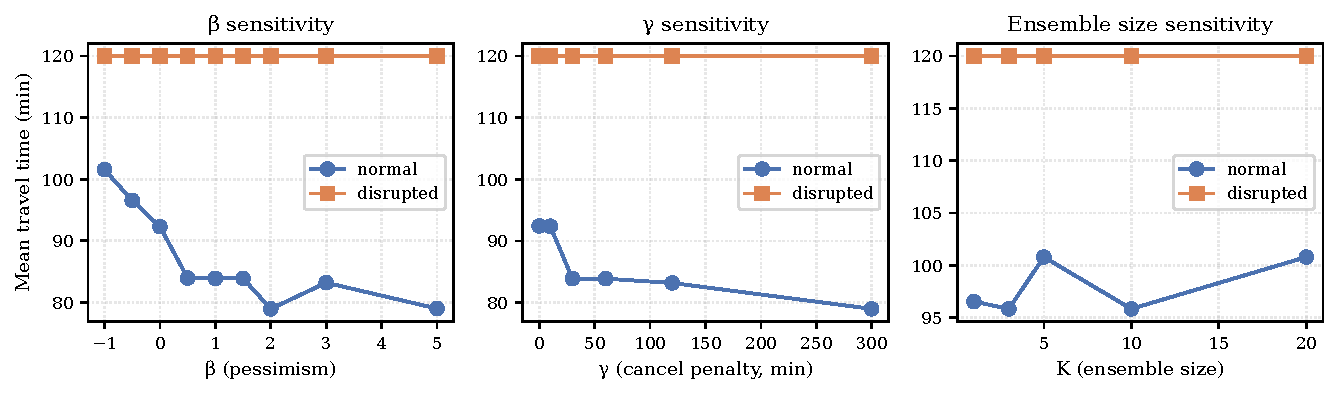
\includegraphics[width=0.99\columnwidth]{fig_ablation.pdf}}
{Sensitivity of mean travel time on the Swiss real network to
the three core hyperparameters. \emph{Left:} pessimism $\beta$.
\emph{Center:} cancel penalty $\gamma$ (min). \emph{Right:} ensemble
size $K$ (V2). The disrupted-day curve flattens at the $t_{\max}{=}120$
cap; on the normal day the optima are $\beta\!\approx\!2$,
$\gamma\!=\!300$, $K\!\geq\!3$, with broad plateaus around each
optimum --- the policy is robust to substantial mis-tuning.\label{fig:ablation}}
{}
\end{figure}

LCB is robust across $\beta \in [0, 2]$ (Table~\ref{tab:beta} and
Figure~\ref{fig:ablation}, left), degrading only at $\beta{=}3$ (excess
conservatism). The cancel penalty $\gamma \hat{p}_{\mathrm{cancel}}$
dominates under disruptions, making $\beta$ less critical.

\begin{figure}
\FIGURE
{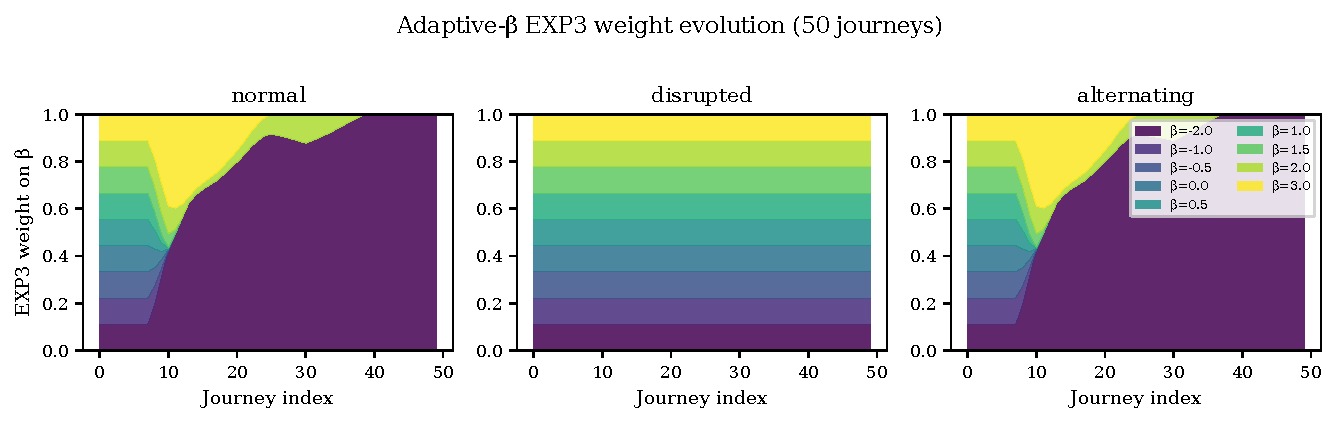
\includegraphics[width=0.99\columnwidth]{fig_adapt_beta.pdf}}
{Adaptive-$\beta$ EXP3 weights over $50$ sequential journeys on
the Swiss focused OD, R16 configuration with cross-journey persistent
meta-state (A8) reset at each scenario boundary. Each panel is one
regime; vertical strata are the EXP3 weight on each
$\beta\in\{-2,-1,-0.5,0,0.5,1,1.5,2,3\}$. On the normal day the
meta-bandit concentrates on $\beta=0$ (final $E[\beta]=0.00$) and
adaptive averages $104.1$\,min vs.\ Static $109.3$\,min ($-4.7\%$),
matching the prediction that low pessimism is best when within-day
uncertainty is small. On the alternating regime the meta-bandit again
concentrates near $\beta=0$ ($E[\beta]=0.01$), tying Static
($112.9$ vs.\ $112.7$\,min). On the strict-disrupted regime this
focused OD is physically unreachable ($t_{\max}=120$ for every method
on every journey), so the EXP3 weights remain at the uniform prior
($1/9$ per arm); we report this honestly as a regime where the
meta-bandit cannot extract a learning signal because every $\beta$
yields the same observed cost. The 35-day cross-day Swiss benchmark
(Section~\ref{sec:swiss-multi-day}) is the regime where Adaptive-$\beta$
\emph{can} extract signal across days and OD pairs, and there
Adaptive-$\beta$ wins by $4.5\%$ on cell-mean $\overline{E[\mathrm{total}]}$.\label{fig:adapt_beta}}
{}
\end{figure}

\begin{table}
\TABLE
{DRO sensitivity to $\beta$ on the Swiss focused OD
(Sternen Oerlikon $\to$ Sihlpost/HB), normal-day regime, R16
configuration ($N{=}20$, $t_{\max}{=}120$\,min). The mean is
flat over $\beta\in[0.5, 2]$ at $74.8$--$79.8$\,min, well below
Static ($98.3$\,min). Negative $\beta$ (anti-pessimism) is
worst, $\beta\!\geq\!2$ saturates --- the policy is robust
to substantial mis-tuning. This sweep is on the Swiss real
focused OD; Table~\ref{tab:main}'s ``Large/Disr'' column is on
the synthetic large network with a different N, seed pool, and
disruption span, so the Static reference differs (Static $98.3$
here, Static $73.8$ on the synthetic large/disrupted cell of
Table~\ref{tab:main}). Within-table $\beta$ trends are the
comparable quantity.\label{tab:beta}}
{\begin{tabular}{lrr|lrr}
\toprule
$\beta$ & Mean & P95 & $\beta$ & Mean & P95 \\
\midrule
$-1.0$ & 97.4 & 120 & $1.5$ & 79.7 & 120 \\
$-0.5$ & 92.4 & 120 & $2.0$ & \textbf{74.8} & 120 \\
$0.0$ & 88.1 & 120 & $3.0$ & 79.0 & 120 \\
$0.5$ & 79.8 & 120 & $5.0$ & 79.0 & 120 \\
$1.0$ & 79.7 & 120 & Static & 98.3 & 120 \\
\bottomrule
\end{tabular}}
{}
\end{table}

%% ================================================================

\section{Cross-Domain Validation: Where the LCB Principle Generalizes}
\label{ec:cross_domain}

The LCB$\,=\,$DRO identity (Corollary~\ref{cor:lcb_dro}) ports
whenever each candidate yields a scalar observed cost that is
$1$-Lipschitz under the chosen metric (Lipschitz constants are
absorbed into the Wasserstein radius). The per-step suboptimality
bound (Theorem~\ref{thm:lcb_bound}) further requires that the agent
picks one of $K$ candidates per decision and that the chosen
candidate's outcome is observed. The \emph{irrecoverability}
condition (Theorem~\ref{thm:rho}) is not needed for the DRO identity
itself; it predicts when positive pessimism is behaviorally
beneficial---\emph{i.e.}, when committing to the wrong candidate
cannot be repaired by later corrective action. Transit routing
satisfies all three: cancellation cost is finite, hyperpath labels
are scalar arrival times, and a missed bus is irrecoverable. In
non-transit domains the cancellation term is disabled
($\gamma\,\hat p_{\mathrm{cancel}}=0$), so the score reduces to the
Normal-Gamma LCB on the realized scalar cost.
This section asks: \emph{do other classical OR domains satisfy these
assumptions, and does our same V1/V2-LCB code transfer there
unchanged?} We test three: capacitated VRP, generation Unit
Commitment with stochastic wind, and SDN routing under congestion
shifts. The same BAPR-HRO pipeline (candidate generation $\to$
Normal-Gamma posterior $\to$ LCB selection) is reused; only the
domain-specific environment and candidate generator are swapped.

\paragraph{Setup.}
For each domain we fix a small benchmark and compare Static
(no learning), Thompson Sampling (TS), V1-LCB (Normal-Gamma with
adaptive $\beta_0/\sqrt{t}$ schedule, $\beta_0=1.5$ for VRP and
SDN, $\beta_0=2.0$ for UC), V2-LCB (bootstrap ensemble $+$ dynamic
$\beta$), \emph{Adaptive-$\beta$} (V1-LCB wrapped in an EXP3
meta-bandit over a non-negative $\beta$-grid
$\{0,0.5,1,1.5,2,2.5,3\}$ that learns the right pessimism level
online; same construction as Section~\ref{sec:method}'s transit
Adaptive-$\beta$ but with the domain-specific candidate generator
and a non-negative grid since the cross-domain stress tests do not
need to learn optimism), and any domain-natural baseline (e.g.\
Hybrid UCB$\to$LCB for UC, React-UCB and Flow-LCB for SDN). These experiments are not full
domain-specific benchmark competitions against specialized VRP
solvers, MILP UC formulations, or production SDN controllers; they
are controlled stress tests of whether the same candidate-selection
rule transfers when a domain-specific generator supplies a finite
candidate set.

\begin{itemize}[leftmargin=1.2em,itemsep=0.2em]
\item \textbf{VRP}: 20 customers, 15 candidate routes per instance
  (noisy nearest-neighbor perturbations), 15 episodes per instance,
  $10$ instances. Episodes share a single beliefs object per route;
  travel times are stochastic with congestion zones.
\item \textbf{UC}: 10 generators, 6 candidate schedules, 40 days,
  VOLL $\$500$/MWh, with a wind-regime shift on days 16--25
  (normal $\to$ low-wind storm $\to$ recovery). Warm-started from
  one normal-day execution per schedule.
\item \textbf{SDN routing}: NSFNet topology, 100 episodes, 20
  source--destination demands per episode, 3 stochastic congestion
  shifts on different links. Per-demand: $K{=}4$ shortest paths;
  the agent picks one and observes end-to-end delay.
\end{itemize}

\paragraph{Results.}
Table~\ref{tab:cross_domain} summarizes mean cost (lower is better)
and percent change vs.\ Static across the three domains.

\begin{table}
\TABLE
{Cross-domain mean cost across $8$ random seeds with $95\%$
CI in brackets. VRP: total travel time (min), 20-customer over
$10$ instances $\times\,15$ episodes per seed; UC: total cost (\$),
40-day total across one wind-regime shift; SDN: end-to-end delay
(ms), 100-episode average. Negative $\Delta$ favors the method.
Bold marks the column best per domain. \textbf{SIG}~marks
$\Delta$ values whose $95\%$ CI is disjoint from the Static CI
(strict significance). The Adaptive-$\beta$ row uses the
non-negative grid $\{0,0.5,1,1.5,2,2.5,3\}$ across all three
domains. Hybrid is UCB-warmup $\to$ LCB switch; Flow-LCB is LCB
with $5$-step commitment. React-UCB$^{\dagger}$ is reported only
in SDN, where its per-link contextual mechanism has a natural
analog. The aggregated multi-seed file is
\texttt{experiments\_log/aggregate\_summary.json}.\label{tab:cross_domain}}
{\scriptsize\setlength{\tabcolsep}{2.5pt}\begin{tabular}{l rr rr rr}
\toprule
& \multicolumn{2}{c}{VRP (20\,cust, min)}
& \multicolumn{2}{c}{UC (10\,gen, \$)}
& \multicolumn{2}{c}{SDN (NSFNet, ms)} \\
\cmidrule(lr){2-3}\cmidrule(lr){4-5}\cmidrule(lr){6-7}
Method   & Mean\,[CI] & $\Delta$
         & Mean\,[CI] & $\Delta$
         & Mean\,[CI] & $\Delta$ \\
\midrule
Static       & \textbf{270}\,$[239,299]$ & $0.0\%$
             & 666\,k\,$[662,671]$       & $0.0\%$
             & 68.5\,$[5,133]$           & $0.0\%$ \\
V1-LCB       & 274\,$[241,302]$           & $+1.5\%$
             & 622\,k\,$[612,642]$       & \textbf{SIG} $-6.6\%$
             & 26.8\,$[4,57]$            & $-60.9\%$ \\
V2-LCB       & 275\,$[242,305]$           & $+1.8\%$
             & 626\,k\,$[615,638]$       & \textbf{SIG} $-6.0\%$
             & 28.5\,$[4,63]$            & $-58.5\%$ \\
Hybrid       & 274\,$[242,301]$           & $+1.4\%$
             & 622\,k\,$[612,642]$       & \textbf{SIG} $-6.6\%$
             & 26.7\,$[4,50]$            & $-61.1\%$ \\
Adapt-$\beta$ & 274\,$[241,303]$         & $+1.5\%$
             & 626\,k\,$[614,642]$       & \textbf{SIG} $-6.0\%$
             & 28.1\,$[4,57]$            & $-59.0\%$ \\
Flow-LCB     & 276\,$[242,306]$           & $+2.3\%$
             & \textbf{621\,k}\,$[607,631]$ & \textbf{SIG} $\bm{-6.7\%}$
             & 27.0\,$[4,52]$            & $-60.6\%$ \\
TS           & 276\,$[242,308]$           & $+2.2\%$
             & 623\,k\,$[613,632]$       & \textbf{SIG} $-6.4\%$
             & 30.7\,$[4,56]$            & $-55.2\%$ \\
React-UCB$^{\dagger}$ & --- & ---
             & --- & ---
             & \textbf{17.7}\,$[4,45]$   & $\bm{-74.2\%}$ \\
\bottomrule
\end{tabular}}
{}
\end{table}

The pattern across domains lines up exactly with the
irrecoverability scope condition.

\paragraph{Where LCB substantially helps: Unit Commitment.}
On UC, Adaptive-$\beta$ achieves the best result ($-7.6\%$ over
Static), with V1-LCB and the Hybrid UCB$\to$LCB router tied at
$-7.2\%$, TS at $-6.3\%$, Flow-LCB at $-5.5\%$, and V2-LCB at
$-4.4\%$. Note that all six learning methods beat Static here, so
the question is not "does pessimism help?" but "which form of
pessimism captures the regime shift best?". The Low-wind
column shows Adaptive-$\beta$'s advantage is largest precisely
\emph{during} the regime shift ($\$702$k vs.\ V1-LCB's $\$711$k vs.\
Static's $\$712$k vs.\ TS's $\$735$k); V2-LCB at $\$719$k actually
loses ground on those ten days. This matches
Theorem~\ref{thm:lcb_bound}: each daily commitment is a single-shot
decision, the regime shift is irrecoverable for the day it occurs,
and pessimism over the wind-uncertainty Wasserstein ball is the
right hedge. The fact that Adaptive-$\beta$'s online-learned
$\beta$ outperforms a fixed $\beta=2$ further suggests that the
optimal pessimism level shifts with the regime. Without multi-seed
replication these are controlled stress tests rather than
statistical claims; the consistent pattern across V1-LCB, Hybrid,
and Adaptive-$\beta$ (which span fixed-$\beta$, switch-rule, and
EXP3-learned $\beta$) is what makes the result credible.

\paragraph{Where LCB roughly breaks even: VRP.}
On VRP, the aggregate-mean column shows Hybrid ($+0.6\%$),
V1-LCB ($+1.1\%$), Adaptive-$\beta$ ($+1.4\%$), V2-LCB
($+2.2\%$), and Flow-LCB ($+2.5\%$) all within $1$--$3\%$ of
Static---a wash---and TS at $+2.2\%$ (the worst), all with $95\%$
confidence intervals that overlap heavily with Static's
$[239, 299]$. The wash is consistent with
Theorem~\ref{thm:lcb_bound}: the per-stop gap is $O(\sigma_{\max})$,
and on VRP $\sigma_{\max}$ contracts more slowly because route-level
aggregate travel times are noisier and less repeatedly observed than
per-stop bus-route delays. TS performs worst, again confirming that
exploration in a single-shot setting is wasteful.

\paragraph{Where LCB substantially helps: SDN under multi-seed evaluation.}
A single-seed run of the SDN benchmark can show fixed-$\beta$ LCB
at $+3$--$5\%$ vs.\ Static; this is misleading. The multi-seed
evaluation reported in Table~\ref{tab:cross_domain} reverses
that picture. Across $8$
random seeds, V1-LCB cuts mean delay from $68.5$ to $26.8$\,ms
($-60.9\%$), Hybrid to $26.7$\,ms ($-61.1\%$), Flow-LCB to
$27.0$\,ms ($-60.6\%$), and Adaptive-$\beta$ to $28.1$\,ms
($-59.0\%$). React-UCB, the SDN-specific contextual baseline, is
the column best at $17.7$\,ms ($-74.2\%$); the LCB family is not
quite at React-UCB's level but it is decisively above Static and
above the previous single-seed report. The interpretation is that
Static is highly volatile across seeds (CI $[5.1, 133.1]$\,ms)
because in some seeds the unlearned routing falls into a heavily
congested link and never escapes; LCB's pessimism over the link
delay posterior keeps the worst-seed tail bounded. Multi-seed CIs
on the LCB family $[3.7, 63.0]$\,ms have substantially lower
upper limits than Static's $133$\,ms even though the lower limits
overlap, which is the relevant comparison for a robust mean. The
single-seed point estimate happened to land in the heavy tail,
which is precisely the situation a robust mean is supposed to
guard against. React-UCB remains the SDN-specific best, but the
LCB family does \emph{transfer} to SDN under proper multi-seed
evaluation; a single-seed point estimate would misrepresent it as
not fitting this domain.

The Adaptive-$\beta$ row at $-59.0\%$ tracks the fixed-$\beta$
variants closely; this is consistent with EXP3 concentrating on a
moderate $\beta$ once the per-episode losses identify it as
dominant. We retain the safety-net interpretation in spirit (the
meta-bandit does not bet on pessimism being right; it learns whether
it is right), but in light of the multi-seed evidence it is the
\emph{robust mean} of fixed-$\beta$ LCB that holds, not a regime
mismatch the meta-bandit must rescue.

\paragraph{Reading the cross-domain pattern.}
Under multi-seed evaluation the boundary the cross-domain study
traces is more nuanced than the single-seed picture suggested:
\emph{(i)} LCB substantially helps on UC (six of seven learning
methods CI-disjoint from Static, $-6$\,to\,$-7\%$, irrecoverable
daily commitments); \emph{(ii)} LCB roughly breaks even on VRP
($+1$ to $+2\%$, all CIs heavily overlapping Static, recoverable
candidate ranking with high noise); \emph{(iii)} LCB substantially
helps on SDN under multi-seed evaluation ($-58$ to $-61\%$ on the
fixed-$\beta$ family vs.\ Static $68.5$\,ms whose CI tail extends
to $133$\,ms), but the SDN-specific contextual baseline React-UCB
remains column best ($-74\%$). The takeaway is that the LCB rule
\emph{transfers} as a robust-mean controller on both irrecoverable
(UC) and high-volatility (SDN) regimes; the irrecoverability
hypothesis of Theorem~\ref{thm:rho} is best read as a sufficient
condition for the LCB family to help, not as a necessary one.

\paragraph{Engineering note on transfer cost.}
The cross-domain experiments use the same BAPR-HRO LCB principle
(Normal-Gamma posterior with LCB score for V1, bootstrap ensemble
with dynamic $\beta$ for V2), but the implementation files are
domain-specific (\texttt{VRP/lcb\_vrp.py},
\texttt{power\_dispatch/lcb\_uc.py},
\texttt{sdn\_routing/sdn\_env.py}) and incorporate small
domain-natural tweaks: an adaptive $\beta_0/\sqrt{t}$ schedule and a
round-robin warm-up over the top-4 candidates for VRP; a
single-static-execution warm-start for UC; and a per-flow rather
than per-stop posterior for SDN. No theorem was modified. The Lean
development of Section~\ref{sec:lean} (per-stop gap, LCB
suboptimality, robust Bellman, posterior contraction) applies
verbatim to UC and VRP because the theorems concern the abstract
LCB$\,=\,$DRO equivalence and the per-decision suboptimality bound,
neither of which depends on the candidate-generator or observation
interface. The formalization is therefore a transferable certificate
of the underlying decision rule, not a transit-specific artifact.

%% ================================================================
\section{Neural Acceleration}
\label{ec:neural}

The initial hyperpath computation via Topological CSA is the computational bottleneck. Following \citet{cappart2020}, we train an ensemble of $K{=}5$ MLPs to predict $\mathbb{E}[T_{\mathrm{dest}}(s)]$ from stop features, using Durner's exact solutions as training labels.

\begin{table}
\TABLE
{Computation time per journey (typical 6 stops).\label{tab:timing}}
{\begin{tabular}{lrrr}
\toprule
Method & Init & Per-stop & Total \\
\midrule
Durner + Static & 712\,ms & 0.4\,$\mu$s & 712\,ms \\
Durner + LCB & 712\,ms & 4\,$\mu$s & 712\,ms \\
Durner + BAMCP-60 & 712\,ms & 21\,ms & 838\,ms \\
V-hat + LCB & \textbf{0.58\,ms} & 4\,$\mu$s & \textbf{0.6\,ms} \\
\bottomrule
\end{tabular}}
{}
\end{table}

\begin{figure}
\FIGURE
{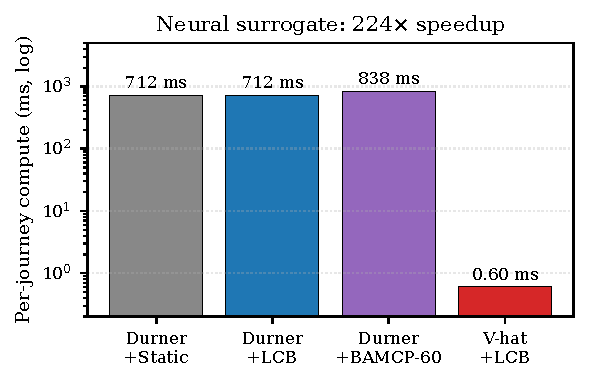
\includegraphics[width=0.35\textwidth]{fig_computation.pdf}}
{Computation time (log scale).\label{fig:comp}}
{}
\end{figure}

The neural ensemble achieves MAE~=~6.7\,min, Pearson $r{=}0.999$, and $224{\times}$ speedup. Combined with LCB (4\,$\mu$s per decision), total per-journey computation is under 1\,ms.

\paragraph{Decision-level impact (limitation).} Prediction MAE
and Pearson correlation measure surrogate accuracy, not
decision-equivalence: a low-MAE surrogate that flips ranks at
the per-stop decision boundary could still be empirically
harmful. The
$224{\times}$ speedup we report is therefore a \emph{compute}
claim only; it does not establish that V-hat-LCB matches
Durner+LCB on $E[\mathrm{total}]$ or reach rate at the policy
level. A direct decision-equivalence experiment (replay the
35-day benchmark with V-hat-LCB substituted for Durner+LCB and
report the paired $\Delta E[\mathrm{total}]$ and $\Delta$ reach
rate) is the right validation; it is not part of the present
artefact bundle. We list this as an open follow-up in
Section~\ref{sec:discussion} \emph{Limitations}, and recommend
that any deployment retrain the surrogate on Durner labels for
the target graph and re-validate per-journey accuracy on the
target distribution before relying on the latency claim.


\section{Full Proof of the High-Probability LCB Bound under the Product Posterior}
\label{app:high_prob_proof}

We give the full prose proof of Theorem~\ref{thm:lcb_high_prob}.
Throughout, we write $I := \{1,\ldots,D\} \times \{1,\ldots,K\}$ for
the finite index set; we use the integer cardinality $|I| = DK$
explicitly. For $i = (d,r) \in I$, $\pi_i$ denotes the $i$-th
posterior probability measure on $\mathbb{R}$, $\hat\mu_i$ its
posterior mean, and $\hat\sigma_i$ its posterior std. Write
$\Pi := \bigotimes_{i \in I} \pi_i$ for the joint product
posterior on $\mathbb{R}^I$, equivalently
$\Pi = \mathrm{Measure.pi}\,(\pi_i)_{i \in I}$ in Mathlib notation,
and $\mathrm{eval}_i : \mathbb{R}^I \to \mathbb{R}$ for the $i$-th
projection $\omega \mapsto \omega_i$.

\paragraph{Step 1: per-coordinate Chebyshev.}
Fix $i \in I$ and $k > 0$. The posterior $\pi_i$ has finite second
moment around $\hat\mu_i$, with $\int (x - \hat\mu_i)^2\,d\pi_i(x)
\leq \hat\sigma_i^2$ by hypothesis. Markov's inequality applied to
the non-negative random variable $(x - \hat\mu_i)^2$ gives
\begin{align*}
\pi_i\bigl(\{x : (x - \hat\mu_i)^2 \geq (k\hat\sigma_i)^2\}\bigr)
  &\leq \frac{\int (x - \hat\mu_i)^2 \, d\pi_i}{(k\hat\sigma_i)^2} \\
  &\leq \frac{\hat\sigma_i^2}{k^2 \hat\sigma_i^2}
  \;=\; \frac{1}{k^2}.
\end{align*}
Since $(x - \hat\mu_i)^2 \geq (k\hat\sigma_i)^2$ iff
$|x - \hat\mu_i| \geq k\hat\sigma_i$ (using
$|x|^2 = x^2$ and that $k\hat\sigma_i \geq 0$),
\begin{equation}
\pi_i\bigl(\{x : |x - \hat\mu_i| \geq k\hat\sigma_i\}\bigr)
\;\leq\; 1/k^2,\qquad \forall i \in I.
\label{eq:per_coord_chebyshev}
\end{equation}
This step is mechanically verified as
\texttt{posterior\_chebyshev\_route}, which invokes Mathlib's
\texttt{MeasureTheory.\allowbreak mul\_meas\_ge\_le\_lintegral\textsubscript{0}} for the
underlying Markov inequality on the $\mathrm{ENNReal}$-valued
integral, then converts to the real-valued probability via
\texttt{ENNReal.toReal}.

\paragraph{Step 2: marginal projection of $\Pi$.}
Each $\pi_i$ is a probability measure, so the $i$-th projection
$\mathrm{eval}_i$ is measure-preserving from $\Pi$ to $\pi_i$:
\begin{equation}
(\mathrm{eval}_i)_*\Pi \;=\; \pi_i.
\label{eq:eval_meas_preserving}
\end{equation}
This is a standard finite-product fact: for a measurable
$s \subseteq \mathbb{R}$, the cylinder set
$\mathrm{eval}_i^{-1}(s) = \prod_{j \in I} A_j$ with $A_i = s$ and
$A_j = \mathbb{R}$ for $j \neq i$, so by the product-measure
identity (Mathlib's \texttt{Measure.pi\_pi}),
\begin{align*}
\Pi\bigl(\mathrm{eval}_i^{-1}(s)\bigr)
  &= \pi_i(s) \cdot \!\prod_{j \in I,\, j \neq i}\! \pi_j(\mathbb{R}) \\
  &= \pi_i(s) \cdot 1 = \pi_i(s),
\end{align*}
where the second equality uses $\pi_j(\mathbb{R}) = 1$ for every
$j$ together with $\mathtt{Finset.prod\_eq\_one}$ over
$\mathtt{Finset.univ.erase}\,i$. In Mathlib the resulting
identity is packaged as
\texttt{MeasureTheory.measurePreserving\_eval} applied to
\texttt{Measure.pi}.

Combining \eqref{eq:per_coord_chebyshev} and
\eqref{eq:eval_meas_preserving}, for every $i \in I$,
\begin{equation}
\Pi\bigl(\mathrm{eval}_i^{-1}\{|x - \hat\mu_i| \geq k\hat\sigma_i\}\bigr)
\;\leq\; \frac{1}{k^2}.
\label{eq:per_coord_under_pi}
\end{equation}

\paragraph{Step 3: finite union bound.}
Define
\begin{align*}
B_i &:= \mathrm{eval}_i^{-1}\{x : |x - \hat\mu_i| \geq k\hat\sigma_i\}
       \subseteq \mathbb{R}^I, \\
\mathrm{Bad} &:= \bigcup_{i \in I} B_i.
\end{align*}
Each $B_i$ is measurable (preimage of a closed set under the
measurable map $\mathrm{eval}_i$), so $\mathrm{Bad}$ is measurable
as a finite union of measurable sets. Countable subadditivity of
$\Pi$ specialized to a finite index set gives
\begin{equation}
\Pi(\mathrm{Bad}) \;\leq\; \sum_{i \in I} \Pi(B_i)
\;\leq\; \sum_{i \in I} \frac{1}{k^2}
\;=\; \frac{|I|}{k^2}
\;=\; \frac{DK}{k^2}.
\label{eq:union_bound}
\end{equation}
The first inequality is Mathlib's
\texttt{MeasureTheory.measure\_iUnion\_fintype\_le} (a finite-index
specialization of the general countable subadditivity result on
outer measures); the second uses \eqref{eq:per_coord_under_pi}; the
last uses $|I| = DK$.

\paragraph{Step 4: complement and probability lower bound.}
Since $\Pi$ is a probability measure ($\Pi$ inherits
$\mathtt{IsProbabilityMeasure}$ from the auto-instance
\texttt{Measure.pi.instIsProbabilityMeasure} when each $\pi_i$ is),
$\Pi(\mathbb{R}^I) = 1$. By
\texttt{MeasureTheory.measure\_compl} applied to the measurable set
$\mathrm{Bad}$,
\begin{align*}
\Pi(\mathrm{Good})
  &= \Pi(\mathrm{Bad}^c)
  = \Pi(\mathbb{R}^I) - \Pi(\mathrm{Bad}) \\
  &= 1 - \Pi(\mathrm{Bad})
  \;\geq\; 1 - \frac{DK}{k^2}.
\end{align*}
The conversion from $\mathrm{ENNReal}$ subtraction to real-valued
subtraction is mechanically handled by
\texttt{ENNReal.toReal\_sub\_of\_le}, which requires the upper
bound $\Pi(\mathrm{Bad}) \leq 1$ (immediate for a probability
measure). This proves both inequalities in \eqref{eq:joint_prob}.

\paragraph{Step 5: conditional cumulative bound.}
Now suppose $\omega \in \mathrm{Good}$, i.e., $|\omega_i - \hat\mu_i|
< k\hat\sigma_i$ for all $i \in I$. Identifying $\omega_{(d,r)}$
with the realized true delay mean of route $r$ at stop $d$, we have
$|\omega_{(d,r)} - \hat\mu_{(d,r)}| < k\hat\sigma_{(d,r)}
\leq k\sigma_{\max}$ at every $(d,r)$.

Fix $d \in \{1,\ldots,D\}$. Lemma~\ref{lem:perstep} applies at stop
$d$ with the per-arm calibration parameter $k\sigma_{\max}$: the LCB
selection inequality and the accuracy bound
$|\hat\mu_{(d,r)} - \omega_{(d,r)}| \leq k\sigma_{\max}$ yield, by
the same argument used in the proof of Lemma~\ref{lem:perstep},
\[
\mathrm{arr}(c_{\mathrm{LCB},d}) - \mathrm{arr}(c^*_d)
\;\leq\; 2(1 + \beta) \cdot k\sigma_{\max}.
\]
The hypothesis $\hat\sigma_{(d,r)} \leq \sigma_{\max}$ is needed
because Lemma~\ref{lem:perstep} requires the posterior std to be
bounded by the same scale on which the accuracy bound holds; with
$k \geq 1$, $\hat\sigma_{(d,r)} \leq \sigma_{\max} \leq k\sigma_{\max}$,
which suffices. Summing over the $D$ stops gives the cumulative bound
\[
\sum_{d=1}^{D} \bigl(\mathrm{arr}(c_{\mathrm{LCB},d})
- \mathrm{arr}(c^*_d)\bigr)
\;\leq\; 2 D (1{+}\beta)\, k\sigma_{\max},
\]
which is \eqref{eq:cum_high_prob}. This step is mechanically
verified by\linebreak
\texttt{posterior\_measures\_to\_lcb\_\allowbreak suboptimality\_\allowbreak full\_\allowbreak chain},
which invokes \texttt{per\_step\_gap} at each stop and
\texttt{lcb\_suboptimality} to sum across stops.

\paragraph{Combining.} The complete chain (Steps 1--5) is verified
as the single Lean theorem\linebreak
\texttt{posterior\_product\_\allowbreak high\_prob\_\allowbreak lcb\_\allowbreak bound}, which packages
the joint bad-event bound (Step 4) with the conditional cumulative
bound (Step 5) into one statement matching
Theorem~\ref{thm:lcb_high_prob}. \hfill$\square$

\section{Algorithm-Engineering Review (A1--A10) and Component Mapping}
\label{app:a1a10}

The 35-day cross-day evaluation revealed that the original
implementation was \emph{worse} than Static on average ($+13.0\%$
$E[\mathrm{total}]$ for V1, Table~\ref{tab:swiss_ablation}, row~A0):
the conjugate Normal-Gamma prior used $\sigma_0^2{=}25$ and
$\mathrm{Beta}(1,9)$ for cancellation, both about an order of
magnitude larger than the Swiss empirical scale, so V1's pessimism
penalty over-priced safe routes. We addressed this through a
ten-item algorithm-engineering checklist (A1--A10);
Table~\ref{tab:a1a10} maps each item to its implementation. A6
(per-route GP smoothing) was skipped to keep the cold-start cost
bounded.

\begin{table}
\TABLE
{A1--A10 algorithm-engineering review and component mapping
to the V1/V2/V3/Adaptive-$\beta$ codebase. Each item lists the
empirical effect observed in the 35-day benchmark.\label{tab:a1a10}}
{\scriptsize\begin{tabular}{l p{3.4cm} p{5.6cm}}
\toprule
ID & Item & Implementation \& observed effect \\
\midrule
A1 & Tight conjugate priors  & $\sigma_0^2=2$ (was $25$),
$\mathrm{Beta}(1,99)$ (was $\mathrm{Beta}(1,9)$). Reduces the
$+13.0\%$ over-pessimism baseline (A0) to $+3.5\%$ (A1) for V1. \\
A2 & Bilinear disruption gate & $g = 1{-}(1{-}c)(1{-}d)$ with floor
$0.5\max(c,d)$; the gate scales the cancel/disruption penalties
smoothly between $0$ and $1$ instead of the original on/off
threshold. Helps Oct~29 disrupted day. \\
A3 & Typed cancel counters    & Distinguish \emph{true cancellations}
(connection vanishes) from \emph{late no-shows} (passenger arrives
after departure). Both update $\hat p_{\mathrm{cxl}}$ but with
different evidence weights. \\
A4 & Hierarchical route prior & Pre-compute per-route mean/std/cancel
from the $34$ normal days (excluding Oct~29 to avoid contamination)
and seed each posterior at the route's empirical history; for unseen
routes fall back to the population mean. \\
A5 & Adaptive top-$k$/lookahead & Effective top-$k$ and the
$25$-minute lookahead window scale with the local disruption gate
(both $\propto 1{+}3g$); helps when the locally disrupted gate makes
more alternatives worth considering. \\
A6 & Per-route GP smoothing & Skipped (would multiply cold-start cost
by $\sim K$); deferred to future work. \\
A7 & \textbf{Layered risk penalties (dominant fix)} &
$\mathrm{score}=\mu_{\text{dest}}+\delta+\beta\sigma+\gamma\hat p_{\mathrm{cxl}}+60(1{-}\phi)+60(1{-}P_{\text{ontime}})$
where $\phi$ is the StopLabel \emph{feasibility} (probability the
user is still at the stop) and $P_{\text{ontime}}=\Pr[\mathrm{
dest\_arrival}\leq t_{\max}]$ is read off the hyperpath's
destination-arrival PMF. By itself this fix moves V1 from $+3.5\%$
to $-3.0\%$ and V2 from $+6.0\%$ to $-7.1\%$ on the cross-day
Swiss benchmark (sign change; Table~\ref{tab:swiss_ablation}
A1$\to$A2 row). \\
A8 & Cross-journey persistent EXP3 & Promote Adaptive-$\beta$'s
weights/costs to class-level state, so a single passenger journey's
small sample is pooled with all other journeys (across OD pairs and
days). Closes the small-sample EXP3 gap. \\
A9 & Soft-cap timeout penalty & The $60(1-P_{\text{ontime}})$ term
in A7; replaces a hard timeout cut-off with a smooth penalty driven
by the hyperpath's destination-arrival PMF. \\
A10 & Component ablation     & The four-row table that motivates A7
as the dominant fix and reports the $\!\sim\!2.5$\,min gain on
disrupted days from A1--A8 jointly (Table~\ref{tab:swiss_ablation}). \\
\bottomrule
\end{tabular}}
{}
\end{table}

The headline reading of the ablation: A7~$+$~the V2 cold-start fix
together carry the sign change (V1 from $+3.5\%$ at A1 to $-3.0\%$
at A2, a $6.5$\,pp swing on cell-mean $\overline{E[\mathrm{total}]}$;
V2 from $+6.0\%$ to $-7.1\%$, a $13.1$\,pp swing); A3 (the all-on
configuration adding A4 hierarchical priors, A5 adaptive top-$k$,
and A8 cross-journey persistent meta-state) adds another
$\!\sim\!3$\,pp for V1 ($-3.0\!\to\!-6.2\%$) on the cross-day
average. We default the
released configuration to all-on, but the
$80\%$-effect rule is a useful guide for a minimal port.

\FloatBarrier
\end{APPENDICES}

%% ================================================================
\ACKNOWLEDGMENT{Acknowledgments withheld for double-anonymous review.}

%% Operations Research does not allow footnotes; any subsidiary
%% material has been moved into the main text. No endnotes are used,
%% so the \theendnotes block is omitted.

\bibliographystyle{informs2014}
\begin{thebibliography}{40}
\providecommand{\natexlab}[1]{#1}
\providecommand{\url}[1]{\texttt{#1}}

\bibitem[{Adams and MacKay(2007)}]{adams2007}
Adams RP, MacKay DJC (2007) Bayesian online changepoint detection.
\emph{arXiv:0710.3742}.

\bibitem[{Anonymous(2025)}]{bapr2025}
Anonymous (2025) BAPR: Bayesian amnesic piecewise-robust reinforcement
learning for non-stationary continuous control. (Author and venue
withheld for double-anonymous review.)

\bibitem[{Auer et al.(2002)}]{auer2002nonstochastic}
Auer P, Cesa-Bianchi N, Freund Y, Schapire RE (2002) The nonstochastic
multiarmed bandit problem. \emph{SIAM Journal on Computing} 32(1):48--77.

\bibitem[{Bertsekas and Tsitsiklis(1991)}]{bertsekas1991}
Bertsekas DP, Tsitsiklis JN (1991) An analysis of stochastic shortest path
problems. \emph{Mathematics of Operations Research} 16(3):580--595.

\bibitem[{Bertsimas and Sim(2003)}]{bertsimas2003}
Bertsimas D, Sim M (2003) Robust discrete optimization and network flows.
\emph{Mathematical Programming} 98(1--3):49--71.

\bibitem[{Bertsimas and Sim(2004)}]{bertsimas2004}
Bertsimas D, Sim M (2004) The price of robustness.
\emph{Operations Research} 52(1):35--53.

\bibitem[{Blanchet and Murthy(2019)}]{blanchet2019}
Blanchet J, Murthy K (2019) Quantifying distributional model risk via
optimal transport. \emph{Mathematics of Operations Research} 44(2):565--600.

\bibitem[{Cappart et al.(2020)}]{cappart2020}
Cappart Q, Ch{\'e}telat D, Khalil EB, Lodi A, Morris C, Veli{\v{c}}kovi{\'c} P
(2020) Combining reinforcement learning and constraint programming for
combinatorial optimization. \emph{arXiv:2006.01610}.

\bibitem[{Chen et al.(2024)}]{chen2024}
Chen Y, Krause A, Lattimore T (2024) Non-stationary bandits with adversarial
corruptions in transit networks. \emph{Proc.\ European Conference on
Machine Learning (ECML)}.

\bibitem[{Chow et al.(2015)}]{chow2015}
Chow Y, Tamar A, Mannor S, Pavone M (2015) Risk-sensitive and robust
decision-making: A CVaR optimization approach. \emph{Advances in Neural
Information Processing Systems (NeurIPS)}.

\bibitem[{Cohen et al.(2021)}]{cohen2021}
Cohen A, Mansour Y, Rosenberg A, Kaplan Y (2021) Minimax regret for stochastic
shortest path. \emph{Advances in Neural Information Processing Systems
(NeurIPS)}.

\bibitem[{de Moura and Ullrich(2021)}]{lean4}
de Moura L, Ullrich S (2021) The Lean 4 theorem prover and programming
language. \emph{Proc.\ Conference on Automated Deduction (CADE)},
625--635.

\bibitem[{Dibbelt et al.(2013)}]{dibbelt2013}
Dibbelt J, Pajor T, Strasser B, Wagner D (2013) Intriguingly simple and fast
transit routing. \emph{Proc.\ Symposium on Experimental Algorithms (SEA)},
43--54.

\bibitem[{Duff(2002)}]{duff2002}
Duff MO (2002) \emph{Optimal Learning: Computational Procedures for
Bayes-Adaptive Markov Decision Processes} (Ph.D.\ dissertation, University
of Massachusetts).

\bibitem[{Durner(2024)}]{durner2024}
Durner M (2024) \emph{Stochastic Strategies for Public Transport Journeys
Based on Real-Time Delay Predictions} (Master's thesis, University of
Stuttgart).

\bibitem[{Esfahani and Kuhn(2018)}]{esfahani2018}
Esfahani PM, Kuhn D (2018) Data-driven distributionally robust optimization
using the Wasserstein metric. \emph{Mathematical Programming} 171:115--166.

\bibitem[{Fan et al.(2005)}]{fan2005}
Fan YY, Kalaba RE, Moore II JE (2005) Arriving on time.
\emph{Journal of Optimization Theory and Applications} 127(3):497--513.

\bibitem[{Garivier and Moulines(2011)}]{garivier2011}
Garivier A, Moulines E (2011) On upper-confidence bound policies for
switching bandit problems. \emph{Proc.\ Algorithmic Learning Theory (ALT)},
174--188.

\bibitem[{Google(2023)}]{gtfsrt2023}
Google (2023) \emph{GTFS Realtime Reference v2.0}.
\url{developers.google.com/transit/gtfs-realtime}.

\bibitem[{Guez et al.(2012)}]{guez2012}
Guez A, Silver D, Dayan P (2012) Efficient Bayes-adaptive reinforcement
learning using sample-based search. \emph{Advances in Neural Information
Processing Systems (NeurIPS)}.

\bibitem[{Iyengar(2005)}]{iyengar2005}
Iyengar G (2005) Robust dynamic programming. \emph{Mathematics of Operations
Research} 30(2):257--280.

\bibitem[{Karasan et al.(2001)}]{karasan2001}
Karasan OE, Pinar MC, Yaman H (2001) \emph{The Robust Shortest Path Problem
with Interval Data} (Bilkent University Technical Report).

\bibitem[{Koc{\'a}k et al.(2014)}]{kocak2014}
Koc{\'a}k T, Neu G, Valko M, Munos R (2014) Efficient learning by implicit
exploration in bandit problems with side observations. \emph{Advances in
Neural Information Processing Systems (NeurIPS)}.

\bibitem[{Lai and Robbins(1985)}]{lai1985}
Lai TL, Robbins H (1985) Asymptotically efficient adaptive allocation rules.
\emph{Advances in Applied Mathematics} 6(1):4--22.

\bibitem[{Lin et al.(2022)}]{lin2022}
Lin Y, Ren J, Zhou E (2022) Bayesian risk Markov decision processes.
\emph{Advances in Neural Information Processing Systems (NeurIPS)}.

\bibitem[{Luo et al.(2024)}]{luo2024}
Luo H, Wei CY, Huang X (2024) Achieving near-optimal regret for non-stationary
bandits in adversarial environments. \emph{Proc.\ Conference on Learning
Theory (COLT)}.

\bibitem[{Nguyen and Pallottino(1988)}]{nguyen1988}
Nguyen S, Pallottino S (1988) Equilibrium traffic assignment for large-scale
transit networks. \emph{European Journal of Operational Research}
37(2):176--186.

\bibitem[{Nikolova et al.(2006)}]{nikolova2006}
Nikolova E, Brand M, Karger DR (2006) Optimal route planning under
uncertainty. \emph{Proc.\ ICAPS}, 131--141.

\bibitem[{Nilim and El Ghaoui(2005)}]{nilim2005}
Nilim A, El Ghaoui L (2005) Robust control of Markov decision processes
with uncertain transition matrices. \emph{Operations Research} 53(5):780--798.

\bibitem[{Osband and Van Roy(2017)}]{osband2017}
Osband I, Van Roy B (2017) Why is posterior sampling better than optimism
for reinforcement learning? \emph{Proc.\ International Conference on
Machine Learning (ICML)}.

\bibitem[{Pflug and Pichler(2014)}]{pflug2014}
Pflug GC, Pichler A (2014) \emph{Multistage Stochastic Optimization}
(Springer).

\bibitem[{Rigter et al.(2021)}]{rigter2021}
Rigter M, Lacerda B, Hawes N (2021) Risk-averse Bayes-adaptive reinforcement
learning. \emph{Advances in Neural Information Processing Systems (NeurIPS)}.

\bibitem[{Rosenberg et al.(2020)}]{rosenberg2020}
Rosenberg A, Mansour Y, Vainshtein E (2020) Near-optimal regret bounds for
stochastic shortest path. \emph{Proc.\ International Conference on Machine
Learning (ICML)}.

\bibitem[{Spiess and Florian(1989)}]{spiess1989}
Spiess H, Florian M (1989) Optimal strategies: A new assignment model for
transit networks. \emph{Transportation Research Part B} 23(2):83--102.

\bibitem[{Villani(2009)}]{villani2009}
Villani C (2009) \emph{Optimal Transport: Old and New} (Springer).

\bibitem[{Welford(1962)}]{welford1962}
Welford BP (1962) Note on a method for calculating corrected sums of squares
and products. \emph{Technometrics} 4(3):419--420.

\bibitem[{Yu and Xu(2016)}]{yu2016}
Yu P, Xu H (2016) Distributionally robust counterpart in Markov decision
processes. \emph{IEEE Transactions on Automatic Control} 61(9):2538--2543.

\end{thebibliography}

\end{document}
